\thispagestyle{plain}
\section{Inferring and perturbing cell fate regulomes in human brain organoids}
\markboth{Inferring and perturbing cell fate regulomes in human brain organoids}{}


\vspace{0.5cm}

Chapter 3 is an adapted version of the article 'Inferring and perturbing cell fate regulomes in human brain organoids', which has been accepted for publication in \textit{Nature} in July 2022. I contributed the computational analyses of the presented single-cell RNA-seq and ATAC-seq data, the development of the Pando R-package for gene regulatory network inference, as well as assistance with culturing organoids.

\vspace{1cm}

\noindent
{\large\textsc{Authors}}

\noindent
Jonas Simon Fleck\textsuperscript{1$*$}, 
Sophie Martina Johanna Jansen\textsuperscript{1$*$}, 
Damian Wollny\textsuperscript{2}, 
Fides Zenk\textsuperscript{1}, 
Makiko Seimiya\textsuperscript{1}, 
Akanksha Jain\textsuperscript{1}, 
Ryoko Okamoto\textsuperscript{1}, 
Malgorzata Santel\textsuperscript{1}, 
Zhisong He\textsuperscript{1\$}, 
J. Gray Camp\textsuperscript{3,4,5\$}, 
Barbara Treutlein\textsuperscript{1\$}

\vspace{0.5cm}

\noindent
$\ast$ Equal contribution\\
\$ Corresponding author

\vspace{1cm}

\noindent
{\large\textsc{Affiliations}}

\noindent
\textsuperscript{1} Department of Biosystems Science and Engineering, ETH Zürich, Basel, Switzerland\\
\textsuperscript{2} Max Planck Institute for Evolutionary Anthropology, Leipzig, Germany\\
\textsuperscript{3} Institute of Molecular and Clinical Ophthalmology, Basel, Switzerland\\
\textsuperscript{4} University of Basel, Basel, Switzerland\\
\textsuperscript{5} Current affiliation: Roche Institute for Translational Bioengineering (ITB), Roche Pharma Research and Early Development, Roche Innovation Center Basel, Switzerland

\vspace{1cm}

\noindent
{\large\textsc{Correspondence}} 

\noindent
Zhisong He (\href{mailto:zhisong.he@bsse.ethz.ch}{zhisong.he@bsse.ethz.ch})\\
J. Gray Camp (\href{mailto:grayson.camp@iob.ch}{grayson.camp@iob.ch})\\
Barbara Treutlein (\href{mailto:barbara.treutlein@bsse.ethz.ch}{barbara.treutlein@bsse.ethz.ch})

\vspace{1cm}

\noindent
{\large\textsc{Author contributions}} 

\noindent
S.J. generated organoids used in this study, with support from J.S.F., R.O. and D.W.. S.J. generated all single-cell transcriptome and accessible chromatin datasets with support from M.Sa.. S.J. performed the CROP-seq and the multiome experiments. J.S.F., D.W., M.Se. constructed CROP-seq vectors. S.J. generated the GLI3 iPSC lines and generated the scRNA-seq data on GLI3 KO organoids with help from D.W.. F.Z., S.J. performed western blots for GLI3. F.Z. performed the Cut\&Tag experiment. S.J., A.J. generated IHC and HCR data. J.S.F. performed the analysis of the scRNA-seq/scATAC-seq developmental time course with support from Z.H., S.J.. J.S.F. developed the Pando R package. J.S.F. analyzed the CROP-seq data with support from Z.H.. S.J., J.S.F. analyzed the GLI3 KO scRNA-seq and multiome data. J.S.F., S.J., Z.H., J.G.C., B.T. designed the study and wrote the manuscript.

\vspace{1cm}

\noindent
{\large\textsc{Preprint link}} 

\noindent
\href{https://doi.org/10.1101/2021.08.24.457460}{https://doi.org/10.1101/2021.08.24.457460}



\subsection{Abstract}
Self-organizing and unguided neural organoids grown from pluripotent stem cells combined with single-cell genomic technologies provide opportunities to explore gene regulatory networks (GRNs) underlying human brain development. Here we acquire single-cell transcriptome and accessible chromatin data over a dense organoid time course covering neuroepithelial formation, patterning, brain regionalization, and neurogenesis, and identify temporally dynamic and brain region-specific regulatory regions. We develop Pando, a flexible framework that incorporates multi-omic data and transcription factor binding site predictions to infer a global GRN describing organoid development. We use pooled genetic perturbation with single-cell transcriptome readout to assess transcription factor requirement for cell fate and state regulation in organoid. We find that certain factors regulate the abundance of cell fates, whereas other factors impact neuronal cell states after differentiation. We show that the transcription factor GLI3 is required for cortical fate establishment in humans, recapitulating previous work performed in mammalian model systems. We measure transcriptome and chromatin accessibility in normal or GLI3-perturbed cells and identify two distinct GLI3 regulomes central to telencephalic fate decisions: one regulating dorsoventral patterning with HES4/5 as direct GLI3 targets, and one controlling ganglionic eminence diversification later in development. Altogether, we provide a framework for how human model systems and single-cell technologies can be leveraged to reconstruct human developmental biology.


\subsection{Main}

The ability to generate complex brain-like tissue in controlled culture environments from human stem cells offers great promise to understand mechanisms underlying human brain development. Cerebral or other unguided neural organoids develop from embryonic stem cells (ESCs) or induced pluripotent stem cells (iPSCs) into a three-dimensional neuroepithelium that self-patterns, regionalizes, and ultimately forms neurons of the different brain regions (\cite{eiraku_self-organizing_2011,lancaster_cerebral_2013,mariani_modeling_2012}). The fate and state of each cell is orchestrated in part through complex circuits of transcription factors (TFs), converging at regulatory elements and interacting with chromatin to enable precise control of gene expression. Single-cell sequencing approaches allow the profiling of gene expression and chromatin accessibility in individual cells, which opens up new opportunities to survey the set of regulatory control features in any given cell type or state (so-called regulomes). Comprehensive mouse and human brain cell atlases can serve as a reference for understanding organoid cell composition and development (\cite{nowakowski_spatiotemporal_2017,trevino_chromatin_2020,la_manno_molecular_2021}). Direct comparisons between organoids and primary counterparts in mouse and human have quantified a remarkable similarity between the neural progenitor and neuronal transcriptome profiles (\cite{camp_human_2015,fleck_resolving_2021,pollen_establishing_2019}). Cerebral organoids have been used to successfully model microcephaly (\cite{lancaster_cerebral_2013}), periventricular heterotopia (\cite{klaus_altered_2019}), autism (\cite{mariani_foxg1-dependent_2015}) and other neurodevelopmental disorders (\cite{klingler_mapping_2021,di_lullo_use_2017}) that may have differential effects on the various human brain regions. However, we do not yet understand the gene regulatory networks (GRNs) that coordinate early human brain development in normal and perturbed conditions.
Research in model systems have identified core signaling factors and gene regulatory programs that orchestrate brain region formation in vertebrates. Initially, extrinsic signals establish an anterior-posterior axis, which triggers additional localized gradients downstream to segment the neural tube into distinct brain regions. Combinatorial activities of morphogens including SHH, WNTs, BMPs, FGFs, NOTCH, Neuregulins and R-spondins converge on transcription factors to execute regionalization. Much of what is known about these pathways regulating brain morphogenesis have been explored in non-human model systems, and it remains unclear how human brain development has diverged from our mammalian ancestors. Moreover, detailed studies of the mechanisms controlling multi-region brain organoids may provide new insight into the process of brain self-organization (\cite{biesecker_greig_2008}).
New single-cell genomic methods enable high-throughput and quantitative analysis of single-cell transcriptomes and accessible chromatin profiles. These features can also be quantified within an individual cell in a multi-omic measurement, providing insight into gene expression and regulation in the same cell. Furthermore, CRISPR-Cas gene editing coupled with single-cell transcriptome readouts (\cite{dixit_perturb-seq_2016,jaitin_massively_2014,datlinger_pooled_2017}) allows pooled genetic perturbation experiments in vivo (\cite{jin_vivo_2020}). These strategies and vector systems, combined with functionalization of human iPSCs with inducible CRISPR-Cas9 systems, provide an opportunity to perturb gene function in cerebral organoids, and systematically assess the effects across human brain regions.
Here we use a multimodal approach to explore cell fate regulation during human early brain development. We first build a regulome from single-cell transcriptome and accessible chromatin profiling data across a cerebral organoid developmental time course. Regulome perturbations using multiplexed in organoid CRISPR perturbation experiments identify effects on regional fate decisions as well as effects on cell states after fate acquisition. Multiome analysis of a critical period of brain region formation in GLI3 knock-out and Sonic Hedgehog Signaling Molecule (SHH) exposed organoids reveals regulatory disruption of dorsoventral telencephalon diversification and with the help of the inferred regulome we distinguish direct and indirect targets of GLI3. Altogether, we establish a regulome perspective to understand and explore early human brain development.


\begin{figure}[b!]
    \centering
	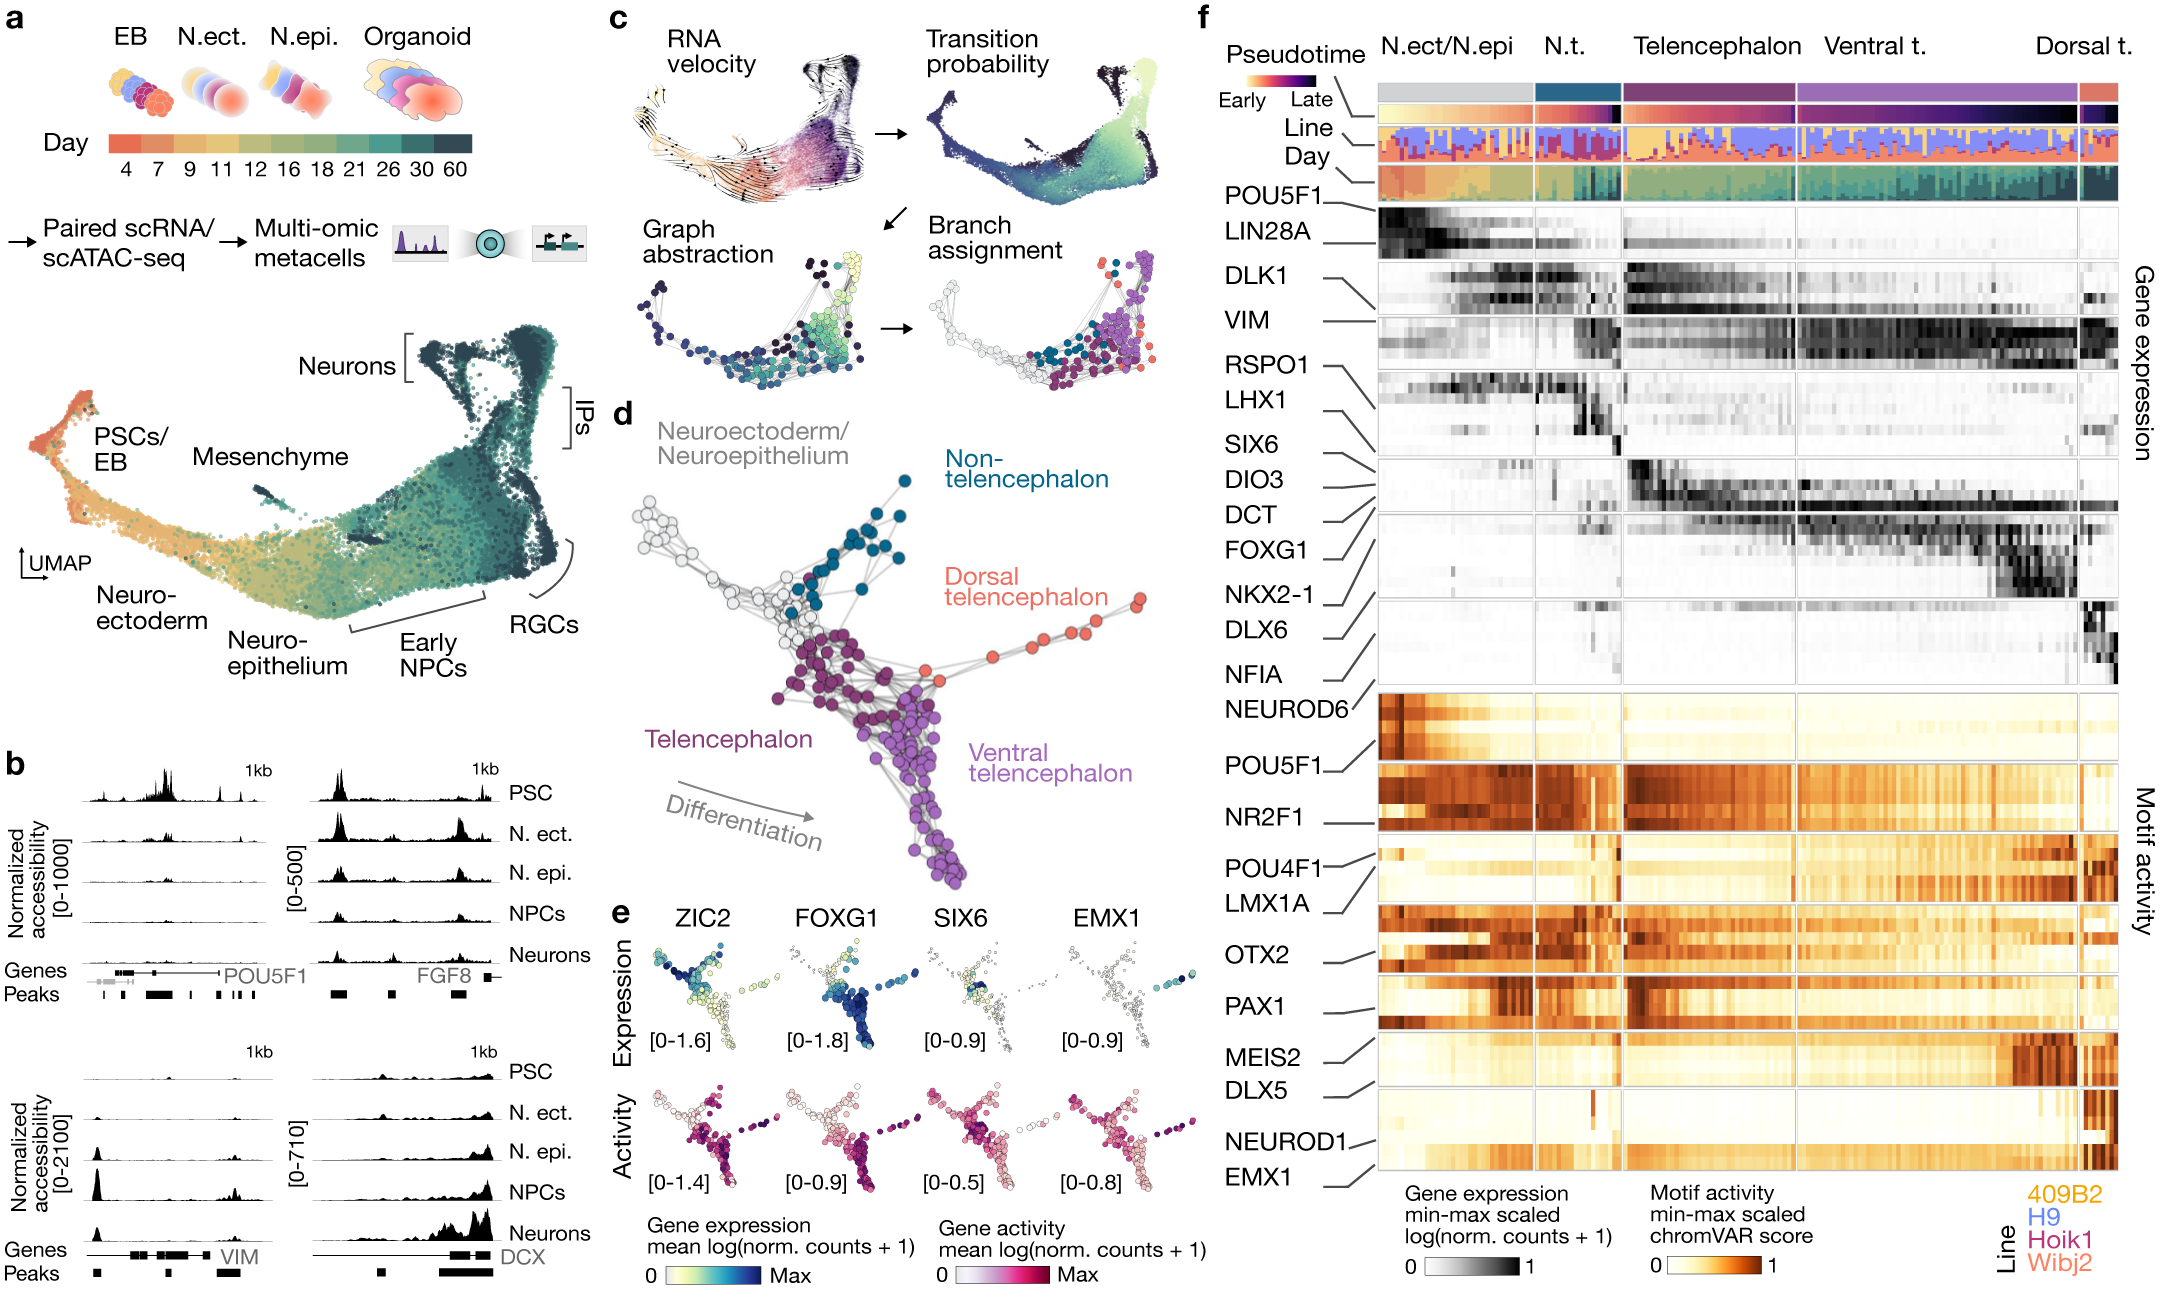
\includegraphics[width=\textwidth]{figures/pando/Figure_1}
    \caption{\textbf{Multi-omic atlas of brain organoid development reveals developmental hierarchies and critical stages of fate decision.}
    a, Schematic of the experimental design and UMAP embedding of integrated multi-omic metacells. Organoids from four different iPSC lines were dissociated for scRNA-seq and scATAC-seq at timepoints spanning the critical patterning window. The two modalities were integrated to form metacells with RNA and ATAC components. b, Examples of loci that have differential access during organoid development from pluripotency. c, Schematic of branch-inference strategy. High-resolution clusters were assigned to branches based on terminal fate transition probabilities calculated based on RNA velocity. d, Branch visualization in a force-directed layout, with circles representing high-resolution clusters of metacells colored by assignment (Neuroepithelium, gray; Non-telencephalon progenitors, teal; Telencephalon progenitors, plum; Dorsal telencephalon, orange; Ventral telencephalon, purple). e, Graph representation of regional branches colored by mean expression (log(transcript counts per 10k + 1)) (top) and gene activity (log(transcript counts per 10k + 1))  (bottom) of marker genes. The range of values is indicated for each plot. f, Heatmap showing stage- and branch-specific gene expression and motif enrichment z-score calculated with chromVAR {Schep et al., 2017}. Values are min-max scaled across rows.}
    \label{fig:reg1}
\end{figure}

\topparagraph{Single-cell multiomic reconstruction of cerebral organoid development}
To explore mechanisms underlying human brain development, we generated single-cell transcriptome and single-cell accessible chromatin profiling data over a time course of cerebral organoid development (Figure 3.1a, Figure S3.1a, Supplementary Table 3.1). The dataset incorporates 11 time points from four human iPSC lines covering two months of development spanning embryoid body (EB) formation, neuroectoderm induction, neuroepithelialization, neural progenitor patterning, and neurogenesis. At each time point, organoid tissues from the four lines were dissociated and scRNA-seq and scATAC-seq pipelines (10X Genomics) were run on the same cell suspension. The sequencing data was demultiplexed using single nucleotide variants (SNVs) specific to each individual and the two modalities for each line and time point were integrated using canonical correlation analysis (CCA) (\cite{stuart_comprehensive_2019}) (Figure S3.1b-f, Supplementary Table 3.2). We constructed ‘multi-omic metacells' containing information on both transcriptome and chromatin accessibility using minimum-cost, maximum-flow (MCMF) bipartite matching (\cite{stark_scim_2020}) within the CCA space (Figure S3.1b,g-h). We evaluated the integration using a multiome dataset, where transcriptome and accessible chromatin were measured within the same cell, and observed strong correlation (Figure S3.1i,j). The metacells were integrated using cluster similarity spectrum (CSS)(\cite{he_css_2020}), and the integrated data was visualized using a Uniform Manifold Approximation and Projection (UMAP) embedding. This revealed a relatively continuous distribution of cell states through the entire time course (Figure 3.1a). Organoid development proceeds from pluripotency (e.g. POU5F1) via a neural progenitor cell state (e.g. PAX6, VIM) to progenitor and neuron cell states of the dorsal telencephalon (e.g. EMX1, NEUROD6), the ventral telencephalon (e.g. DLX5, ISL1, GAD1), of non-telencephalic regions (e.g. TCF7L2, LHX9), and of a small mesenchymal population (e.g. DCN, COL5A1), with cells from the different lines largely intermixed (Figure S3.1f,k). The high-dimensionality of the data could be used to identify marker genes and gene regulatory regions for the different cell states (Figure 3.1b, Figure S3.1l, Supplementary Table 3.3). We observed a pseudotemporal cascade of chromatin accessibility changes over the developmental time course associated with genes involved in stem cell maintenance, neural tube patterning, morphogenesis, neural precursor proliferation, neuron fate specification, and other relevant biological processes (Figure S3.1m, Supplementary Table 3.4).

Previous studies have described the emergence of patterning centers within the neuroepithelium which coordinate to regionalize the developing organoid (\cite{renner_self-organized_2017}). To reconstruct the earliest events involved in cell fate restriction, we sub-clustered early portions of the trajectory and identified molecular heterogeneity (Figure S3.2). In the initial stages (day 7-9), we observed a predominant neuroectodermal population (SIX3, CDH2, SOX3, HES5) and a minor population of cells expressing non-neural ectoderm markers (DLX5, TFAP2A)(\cite{mittnenzweig_single-embryo_2021,ealy_single-cell_2016}) (Figure S3.2a-c). After day 9, cells differentiate into a neuroepithelial population (LDHA), which later diverges into neural progenitor cells (NPCs) expressing either telencephalic (FGF8) and non-telencephalic markers (WLS, WNT8B), followed by a second divergence into dorsal (BMP7, EMX1) and ventral telencephalic NPCs (DLX2; Figure S3.2d-f). RNA fluorescent in situ hybridization (RNA-FISH) using hybridized chain reactions (HCR) of whole-mount 18 day old organoids confirmed the expression and spatial segregation of some of these regional markers (Figure S3.2g).

To assess neuroepithelial self-patterning variation across stem cell lines, we collected additional single-cell multiome data including transcriptome and accessible chromatin modalities for a total of 9 lines (iPSCs: 409B2, B7, HOIK1, KUCG2, WIBJ2, WTC; ESCs: H1, H9, HES3) (~3 weeks; Figure S3.3a). Heterogeneity analysis and comparison with a single-cell transcriptomic atlas of the developing mouse brain6 revealed transcriptionally distinct clusters organizing along an anterior-posterior axis (Figure S3.3b). These clusters expressed many transcription factors, secreted ligands and surface receptors associated with patterning centers such as hypothalamic floor plate (SIX6, HES5, SIX3), roof plate (FGFR3, RSPO3, WNT7B) and hindbrain roof plate (MSX1, BAMBI, BNC2; Figure S3.3c). Notably, marker expression was consistent between lines, however cluster proportions varied substantially, consistent with previous reports(\cite{kanton_organoid_2019}). We further identified cluster-specific candidate cis regulatory elements (CREs) of patterning-related genes and found that many were similarly accessible across lines (Figure S3.3d). These data suggest interesting variation between lines in the propensity to self-pattern, and also support a preserved GRN underlying brain region formation.

We next sought to reconstruct the neurogenic differentiation trajectories for each brain region. We used RNA velocity (\cite{manno_rna_2018,bergen_generalizing_2020}) and CellRank (\cite{lange_cellrank_2022}) to generate a terminal fate transition probability matrix based on transcriptomes, which we used to construct a differentiation graph of high-resolution metacell clusters and assign branch identities (Figure 3.1c, Figure S3.4a-e). The graph, presented by a force-directed layout, reveals an early bifurcation into anterior telencephalic and posterior non-telencephalic cell states and later branching of telencephalic progenitors into dorsal excitatory and ventral inhibitory neuronal trajectories, respectively (Figure 3.1d,e). This telencephalic progenitor state prior to dorsoventral divergence is marked by the expression of DCT, DIO3 and SIX6 and is characterized by transient accessible chromatin regions (Figure 3.1f). Transcriptional and regulatory dynamics can be explored along each neurogenic trajectory, revealing regional specificity of gene expression, chromatin accessibility and binding motif enrichment for stage-specific transcription factors (Figure 3.1f, Figure S3.4f,g). Altogether, this data provides a multi-omic developmental atlas spanning the course of brain organoid regionalization and neurogenesis.
 


\topparagraph{A gene regulatory network view of human cerebral organoid formation}
To infer the GRN underlying human cerebral organoid development, we developed an algorithm called Pando (Figure 3.2a, see Methods), which leverages multi-modal single-cell genomic measurements and models gene expression through TF-peak interactions. Pando first identifies candidate regulatory regions that show accessibility across the organoid time course by incorporating information on conservation (\cite{siepel_evolutionarily_2005}) and previous cis-regulatory element (CRE) annotations (\cite{encode_project_consortium_expanded_2020}) (candidate regions, Figure S3.5a,b). We performed Cleavage Under Targets and Tagmentation (CUT\&Tag) of the H3K27ac histone modification marking active promoters and enhancers to assess regulatory region selection performance. We found that 94\% of accessible peaks intersecting with H3K27ac were among the candidate regions, indicating a strong enrichment for active regulatory regions (Figure S3.5a). 
\begin{figure}[t!]
    \centering
	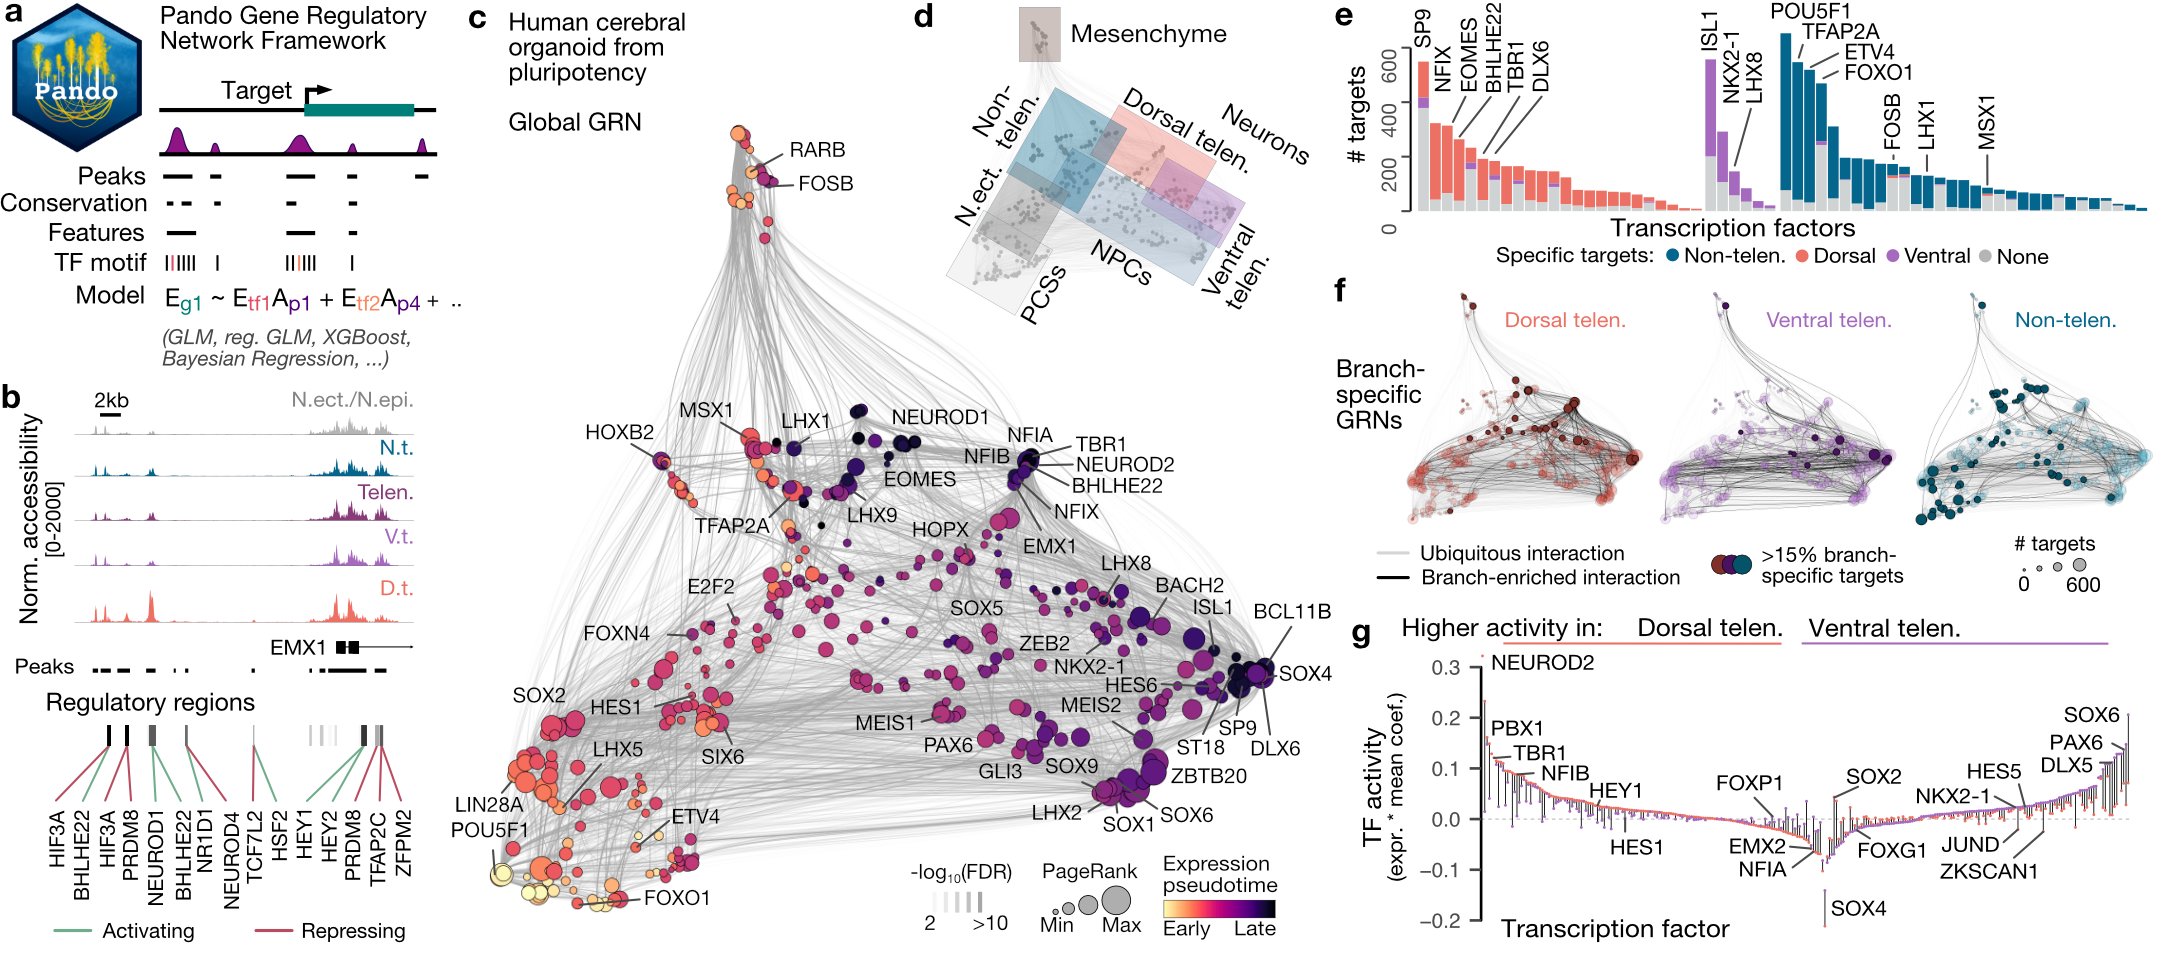
\includegraphics[width=\textwidth]{figures/pando/Figure_2}
    \caption{\textbf{Pando leverages multimodal measurements to infer a multi-phasic gene regulatory network underlying human brain organoid development.}
    a, Schematic of the Pando GRN-inference framework. Candidate regions are identified through intersection of accessible peaks with cis-Regulatory Elements (CREs) or conserved elements. Predicted TFs are selected for each candidate region through binding motif matching. The relationship between TF-binding site pairs and expression of target genes is then fit with a regression model. b, Signal tracks showing normalized accessibility at the transcription start site of EMX1 in the different branches and inferred regulatory regions for various transcription factors. Line color represents the sign of the interaction and box color (grayscale) represents the FDR of the most significant interaction for this region. c, UMAP embedding of the inferred TF network based on co-expression and inferred interaction strength between TFs. Color and size represent expression weighted pseudotime and PageRank centrality of each TF, respectively. d, UMAP embedding shaded by module features. e, Barplots showing target specificity for branch-specific TFs. f, UMAP embedding of branch-specific TF networks highlighting TFs with branch-specific targets and interactions with branch-specific accessibility. g, Plot shows groups of TFs with differential activity between the dorsal (red) and ventral (purple) telencephalon branch. TF activity is indicated by a colored dot for each branch, connected by a line, and was calculated by multiplying the mean regulatory coefficient with the average expression in the branch. The sign of the activity indicates whether the regulation is mainly activating (+) or repressing (-).}
    \label{fig:reg2}
\end{figure}
Next, candidate regions are assigned to genes in their vicinity and TF binding sites are predicted for each region (Figure S3.5c-e). Linking regulatory regions to genes based on proximity has limitations, however it is an effective assumption for many regulatory interactions at the genome scale (\cite{mclean_great_2010,aibar_scenic_2017}), and we observed strong correlation between gene expression and a regulatory domain that includes proximal promoter and gene body regions (Figure S3.1i). Pando then uses a regression model to infer the relationship between the expression of each target gene, TF expression and binding site accessibility (Figure 3.2a, Figure S3.5f). As a consequence, Pando jointly infers sets of positively or negatively regulated target genes (gene modules) as well as regulatory genomic regions (regulatory modules) for each TF (Figure 3.2b, Figure S3.5g-i). We visualized the GRN using a UMAP embedding, which revealed groups of TFs that are involved in different phases of cerebral organoid development, broadly representing the pseudotemporal order of cell state transitions (Figure 3.2c). A series of TFs tracked transitions from pluripotency (e.g. POU5F1, LIN28A) to neuroepithelium induction (e.g. SOX2, HES1), with additional module neighborhoods linked to brain regional NPC specification and neuron differentiation (Figure 3.2d, Figure S3.5j,k). Nodes associated with initializing (pluripotency) and terminal states (regionalized neurons) had a high degree of centrality, reflecting the high number of correlated expressed genes for these states. We found certain TF modules to be pseudotime-dependent independent of brain regional identity (e.g. SP9, SCRT1), whereas others showed specificity for a given brain region (e.g. EMX1, NR1D1, NEUROD6 in dorsal telencephalon; IRX5 in non-telencephalon) (Figure S3.5j,k). Globally, this GRN shows that regulatory region accessibility and TF expression track with stages of organoid development and segregate during brain regionalisation.

To better understand how chromatin accessibility constrains and specifies GRN activity in different brain organoid regions, we next analyzed differential accessibility of inferred binding sites between regional branches. We pruned regulatory edges with strongly depleted accessibility and could identify TFs with highly branch-specific target sets (Figure 3.2e). We further partitioned the global GRN into branch-specific GRNs (Figure 3.2f), representing subgraphs whose activity is shaped by changes in chromatin accessibility between branches. Within these subgraphs, we computed TF activity as the mean coefficient of all active connections multiplied by the mean expression in the branch (Fig 2g). Comparing TF activity in the dorsal and ventral telencephalon branch revealed TFs with high branch-specificity (e.g. NEUROD2, NFIA, SOX6) as well as TFs whose mode of regulation changed between mainly activating (positive activity) to mainly repressing (negative activity; e.g. HEY1, JUND, ZKSCAN1) and vice versa (e.g. SOX2). Altogether, these analyses provide a rich resource for future work to understand the gene regulatory programs controlling human brain regionalization and TF-mediated cell programming.


\topparagraph{Single-cell genomic perturbation of cortical transcription factors in organoids}
To begin to understand the mechanisms regulating cell fate and state during human brain development, we employed a pooled perturbation screen17 in mosaic organoids (Figure 3.3a). We designed gRNAs and generated a pooled lentiviral library targeting 20 TFs (each targeted by 3 gRNAs) expressed in different stages of both organoid and primary developing human cortex7 and with no expression in iPSC or neuroectoderm stages (Figure 3.3b, Figure S3.6a,b). We transduced iPSCs harboring an inducible Cas9 cassette with the lentiviral gRNA library, and sorted and expanded vector positive iPSCs based on fluorescence (Figure S3.6c). We induced Cas9 expression in the infected iPSCs expressing different gRNAs, and used the mosaic pool of iPSCs to generate mosaic cerebral organoids containing a multitude of perturbed genotypes. Fluorescence was maintained throughout organoid development, and bulk amplicon sequencing revealed relatively homogenous detection of the gRNAs (Extended Data Figs. 6d and 7a). At day 60, at which neural progenitors and neurons coexist in the organoid and all targeted TFs have been or are being expressed (Figure 3.3b and Figure S3.6a-b), we dissociated the mosaic organoids and sequenced single-cell transcriptomes and guide cDNA amplicons of 3 individual organoids as well as a pool of multiple organoids. We recovered 22,449 cells with an assigned gRNA. Each gRNA for all 20 targets was detected with an average of 1 gRNA detected per cell (Figure 3.3c, Figure S3.7b-e). We generated a UMAP embedding, analyzed cell type heterogeneity, and annotated NPCs, intermediate progenitors, and neurons in the dorsal telencephalon, the ventral telencephalon, as well as in non-telencephalic developing brain regions (Figure 3.3d, Figure S3.7f-i).

\begin{figure}[b!]
    \centering
	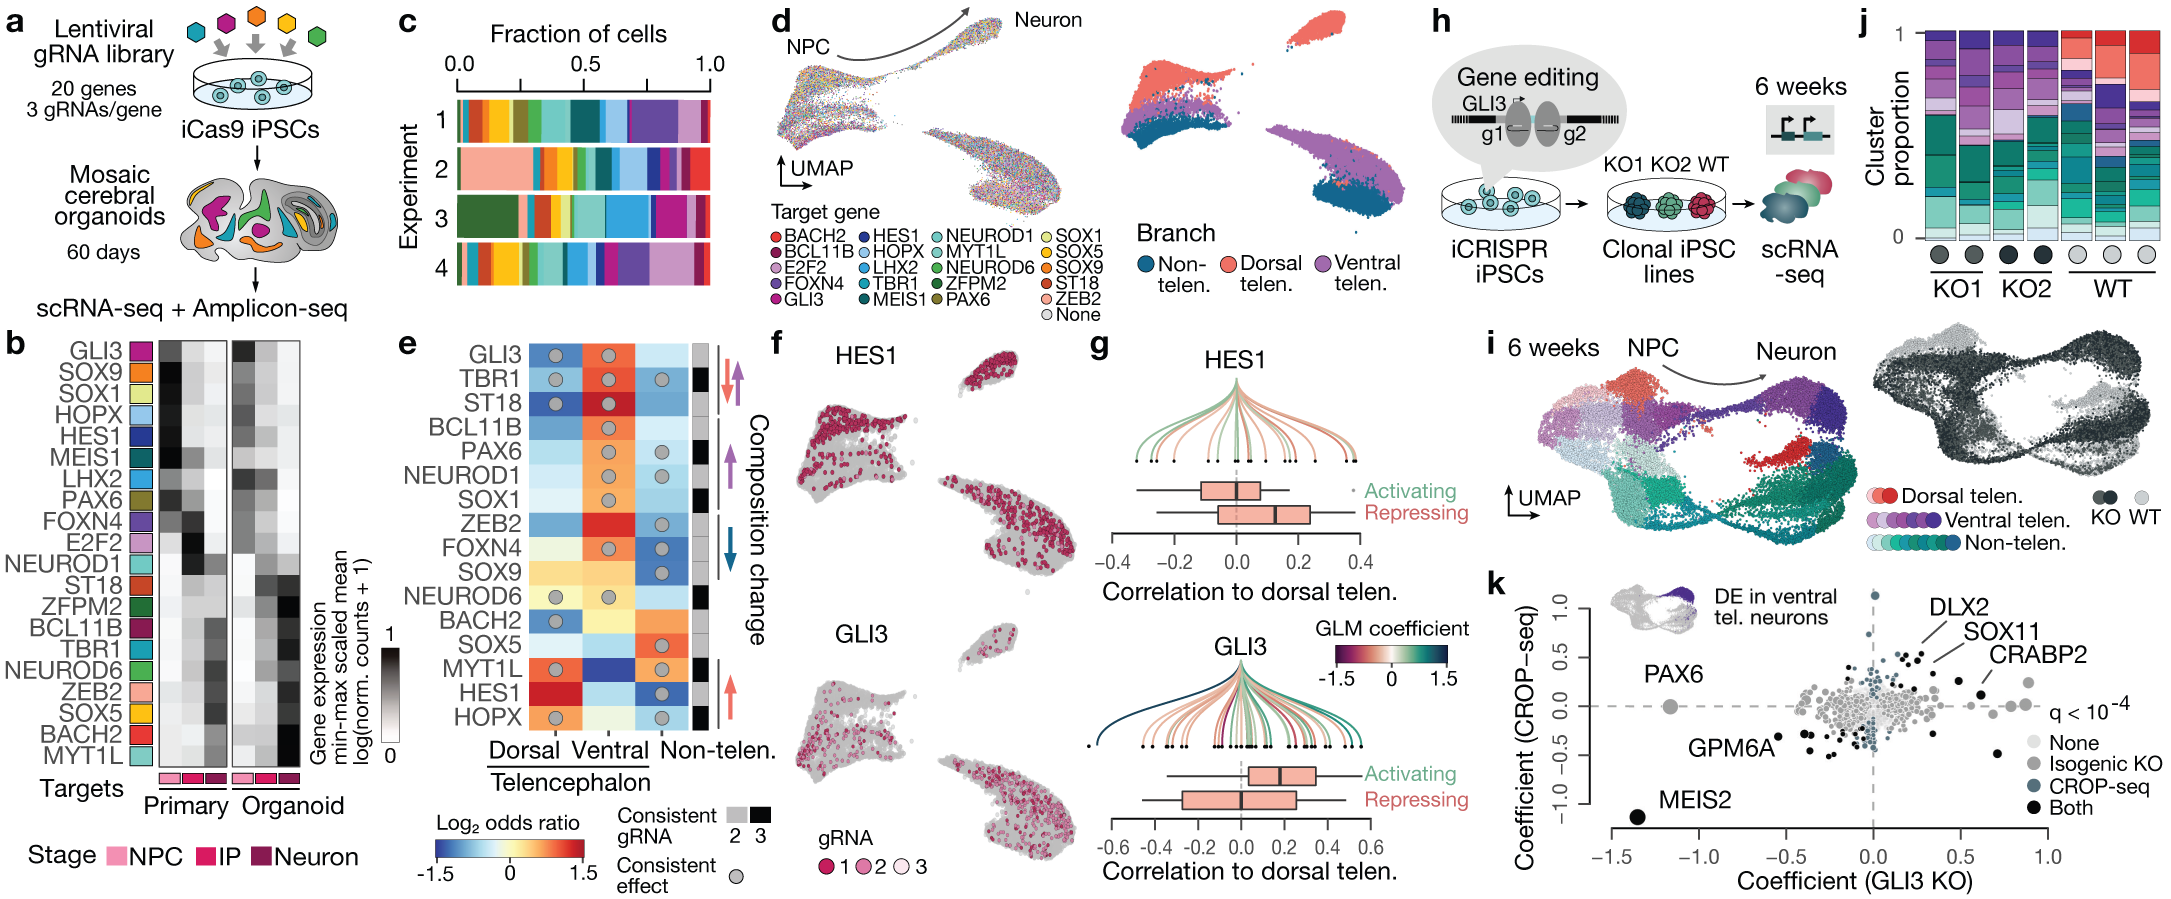
\includegraphics[width=\textwidth]{figures/pando/Figure_3}
    \caption{\textbf{Transcription factor perturbations in mosaic organoids reveal critical regulators of neurodevelopmental fate decisions.}
    a, Schematic of single-cell perturbation experiment using the CROP-seq method and data analysis. b, Heatmap showing min-max scaled average expression (log(transcript counts per 10k + 1)) of targeted genes in neural progenitor cells (NPC), intermediate progenitors (IP) and neurons of the primary and organoid cortex. c,  Barplot showing the proportion of cells with each perturbation for each experiment. d, UMAP embedding with cells colored by detected gRNA (left) and branch assignment (right). e, Heatmap showing regional enrichment of gRNAs. Sidebar shows the number of gRNAs that were consistent and circles represent consistent effects between experiments and statistically significant (FDR<0.01) effects on composition. Arrows indicate the predominant observed effect. f, UMAP embedding colored by consistent gRNAs for selected genes that had a strong effect on fate regulation. g, Box plots showing the spearman correlation of HES1 (top, n=18 genes) and GLI3 (bottom, n=42 genes) target genes to transition probabilities into the dorsal branch. The GRN was subsetted to retain connections accessible at the branchpoint (>5\% detection rate). The center line represents the median, boxes indicate the 25\%-75\% interquantile range and whiskers indicate 1.5 * interquantile range. h, Schematic of GLI3 loss of function experiment (knock-out, KO; wild-type, WT) using the iCRISPR nickase system. i, UMAP embedding showing trajectories from neural progenitor cells (NPCs) to neurons colored by different clusters assigned to regional branches, with inset colored by genetic condition. j, Stacked barplots showing distribution of cluster assignment per organoid for each condition, colored by cluster. k, Differential expression (DE) in ventral telencephalic neurons for GLI3 KO and CROP-seq data containing a GLI3 gRNA. X and y axes indicate coefficients of the linear model. Colors indicate significance (FDR<$10^{-4}$) in CROP-seq, KO cell line, or both.}
    \label{fig:reg3}
\end{figure}

We tested the association of gRNA detection on cell type abundance and on differential gene expression within cell types (Figure S3.8). We first hierarchically clustered Louvain clusters based on gRNA abundance and observed grouping by brain region (Figure S3.8a). This showed that different brain regions exhibited unique gRNA compositions suggesting region specific effects of TF perturbations. Next, we stratified the detected gRNAs using a log odds ratio (p-value based on a Cochran–Mantel–Haenszel test) and assessed the consistency of the effect across organoids and gRNAs (Figure S3.8b, Supplementary Table 3.5). Based on these metrics, we found that gRNAs targeting 8 TFs showed consistent enrichment in the ventral telencephalon branch with corresponding depletion in the other regions, including the cortex (Figure 3.3e; e.g. GLI3, TBR1). Another set of perturbations showed the opposing effect, with enrichment of TF targeting gRNAs in the cortex and depletion in either ventral telencephalon or non-telencephalon (e.g. HES1, HOPX). We focused on HES1 and GLI3, two genes which are expressed at the dorsoventral branchpoint and show opposing effects on dorsal telencephalon commitment (Figure 3.3e,f). Both genes are known regulators of mouse cortical development (\cite{nakamura_bhlh_2000,wang_gli3_2011,hasenpusch-theil_gli3_2018}), and are associated with developmental disorders in humans (\cite{song_non-coding_2021,biesecker_greig_2008}). We used the GRN inferred from the developmental time course to investigate how GLI3 and HES1 target gene expression correlates with transition probabilities into dorsal telencephalon (Figure 3.3g). We found that genes activated by GLI3 were positively correlated with cortical transition probabilities, while HES1 had a repressive effect on such genes. This suggests an antagonistic involvement of these two genes in shaping the dorsoventral fate decision in the human telencephalon. Of note, we also found that for several TFs perturbation led to detectable transcriptomic effects rather than composition changes (Figure S3.8c-f, Supplementary Table 3.6 and 7). In particular, E2F2, a crucial cell cycle regulator (\cite{swiss_cell-context_2010}), altered the transcriptome of both dorsal and ventral telencephalic neurons suggesting that misregulation of cell cycle exit has a large effect on the neuronal transcriptome state. Altogether, these data provide one of the first implementations of an in organoid multiplexed perturbation experiment to explore the effect of genetic perturbations on human brain cell fate and state development.


\topparagraph{GLI3 directly targets HES regulomes during human organoid telencephalon development}
Mosaic perturbations suggested that GLI3 is involved in dorsoventral neuronal fate specification in the human telencephalon. GLI3 is a well known mediator of Sonic Hedgehog (SHH) signaling (\cite{ruiz_i_altaba_hedgehoggli_2002}), with GLI3 loss of function mutations resulting in failure of the cortex to form in mice, and expansion of ventral telencephalic neuronal identities into dorsal locations within the developing brain (\cite{rallu_dorsoventral_2002,theil_gli3_1999}). In humans, mutations in GLI3 have been associated with Greig cephalopolysyndactyly syndrome and Pallister Hall syndrome, in which patients have variable presentations of brain malformations depending on the particular mutations (\cite{biesecker_greig_2008}). To confirm that GLI3 is involved in cell fate establishment in a human context, and to explore the underlying developmental mechanisms, we used CRISPR/Cas9 gene editing to generate two independent GLI3 knock-out (KO) iPSC lines  and a control cell line (WT) that went through the editing process (Figure 3.3h, Figure S3.9a-d). We generated KO and WT cerebral organoids and confirmed that the GLI3 protein is not detected in the KO organoids (Figure S3.9e). We performed scRNA-seq on KO and WT organoids at day 45, a time point of early neurogenesis, and analyzed cellular heterogeneity (Figure 3.3i, Figure S3.9f). Strikingly, KO cells were depleted in the dorsal telencephalon, with a strong enrichment in the ventral telencephalon (Figure 3.3j), and differential gene expression analysis revealed that GLI3 KO impacts ventral telencephalic cell states (Figure 3.3k, Supplementary Table 3.8). Both of these observations were consistent with the mosaic perturbation experiment.


\begin{figure}[b!]
    \centering
	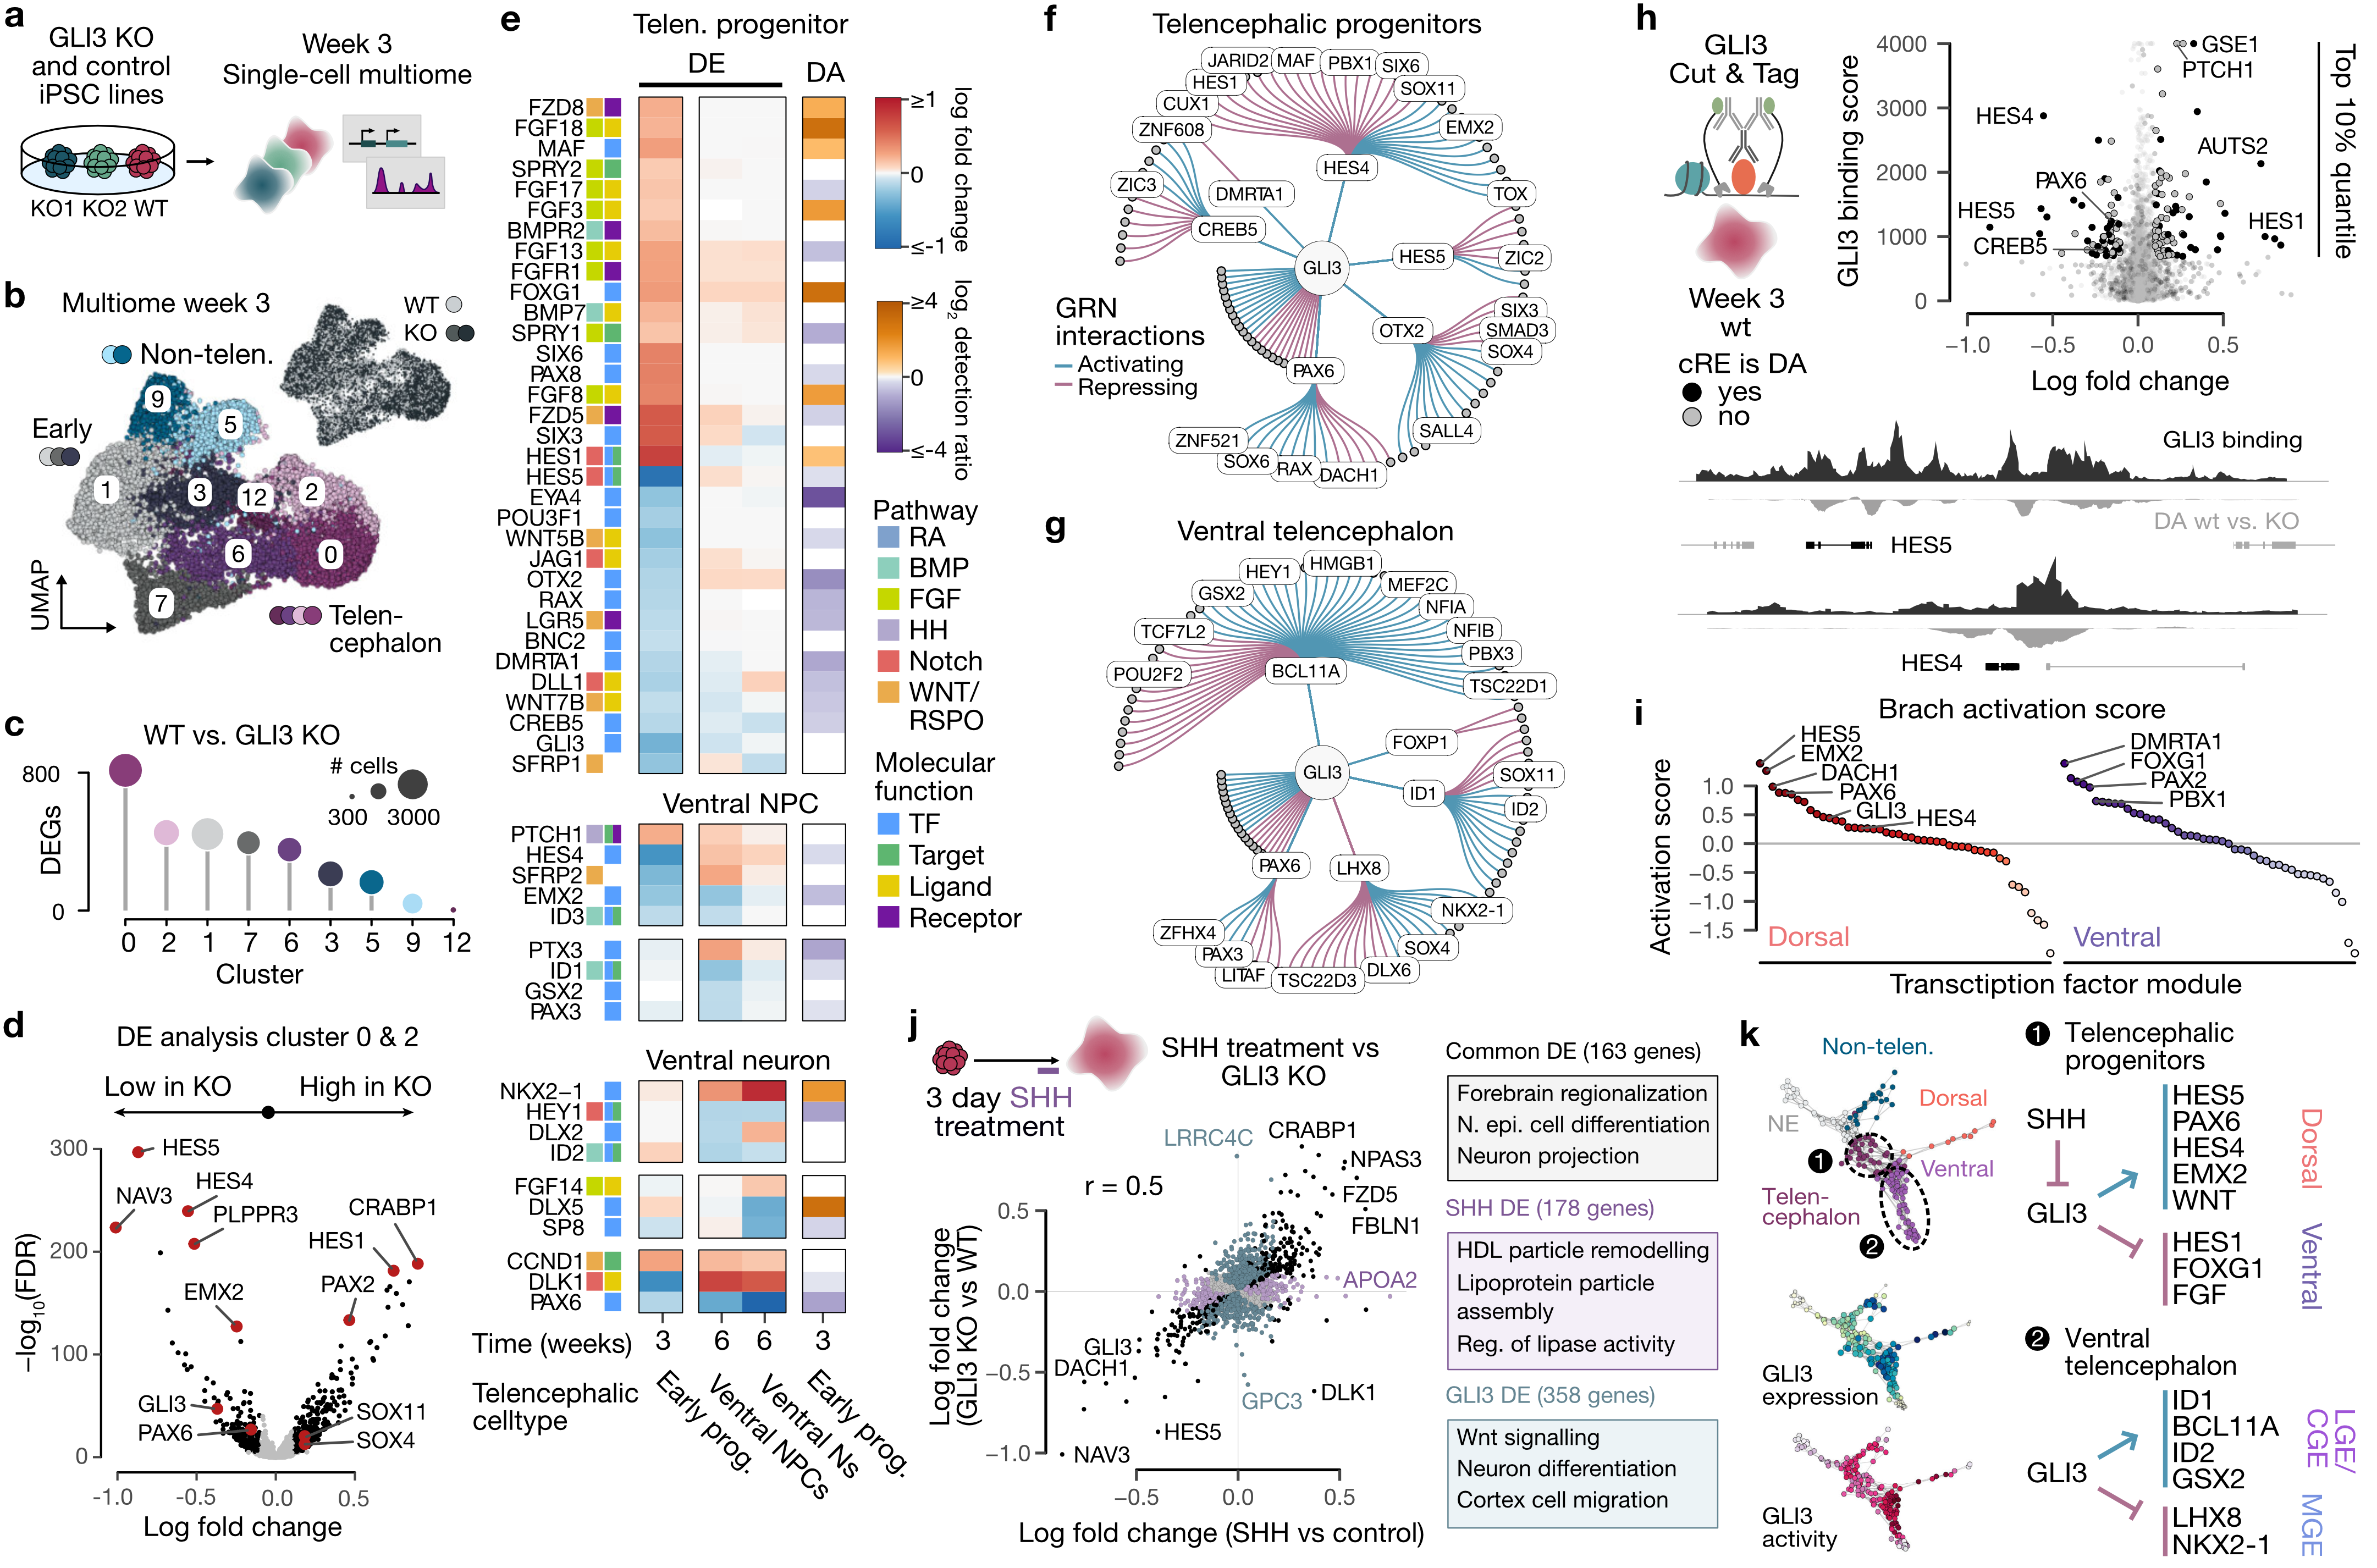
\includegraphics[width=\textwidth]{figures/pando/Figure_4}
    \caption{\textbf{Single-cell multiome view of GLI3 loss of function reveals distinct regulomes and novel effectors of dorsoventral telencephalon specification.}
    a, Schematic of the experiment where transcriptome and chromatin access was measured in the same cell at 3 weeks of cerebral organoid development. b, UMAP embedding colored by cluster and labeled by projected cell fate. Inset UMAP colored by genetic state. c, Lollipop plot showing number of DEGs of control (WT) versus GLI3 KO cells in the different clusters. d, Volcano plot showing DE in telencephalic progenitors (cluster 0 and 2) upon GLI3 KO. e, Heatmap showing DEGs upon GLI3 KO for early telencephalic progenitors (week 3), ventral telencephalic progenitors (week 6) and neurons (week 6), and differential accessibility (DA) upon GLI3 KO in early telencephalic progenitors (week 3). All genes are colored by the related signaling pathway (if applicable) and molecular function. f,g, Subgraph of the GRN for early telencephalic progenitors (f) and in the ventral telencephalon (g), showing direct and second-order GLI3 targets. Circles are genes with all TFs being labeled. Edges are colored based on regulatory interaction by the TF. h, GLI3 binding score (sum of C\&T signal intensity for gene body + 2kb) in WT organoids versus DE log fold change in early telencephalic progenitors (week 3). Genes with differentially accessible Cis-regulatory elements (CREs) are colored black. Signal tracks of GLI3 binding matched with DA peaks of HES4 and HES5 in early telencephalic progenitors. i, Z-scored mean correlation between module genes expression and branch probabilities (branch activation score) for DE TFs. j, Scatterplot showing log fold change of genes upon treatment with SHH versus DE in GLI3 KO. GO terms are shown for common DEGs, SHH treatment specific and GLI3 specific DEGs. k, Schematic summarizing the results from GLI3 and SHH perturbations.}
    \label{fig:reg4}
\end{figure}


Interestingly, the TF MEIS2, a marker of lateral/caudal ganglionic eminence (LGE/CGE) relative to medial ganglionic eminence (MGE), was strongly down-regulated in GLI3 KO conditions (Figure 3.3j). Further analysis on the ventral telencephalic neuron heterogeneity identified distinct LGE/CGE-like and MGE-like neuronal populations with GLI3 KO cells strongly enriched in MGE neurons (Figure S3.9g,h). We observed expression alterations in GLI3 KO LGE-like neurons compared to the WT LGE state with genes involved in dorsoventral patterning (PAX6, MEIS2, DLK1) being differentially expressed (Figure S3.9h). These data confirm that GLI3 is necessary for cortical neuron fate establishment in humans, and its absence impacts ventral telencephalon development by promoting MGE neurogenesis and altering LGE neuronal expression, consistent with a role in MGE fate repression (\cite{sousa_sonic_2010}) and LGE neuron state regulation (Figure S3.9h,i).
GLI3 is expressed broadly in progenitors of the telencephalon and of non-telencephalic regions (Figure S3.4f), suggesting distinct GLI3 regulatory roles during different phases of brain development. We therefore generated single-cell multiome data (10X Genomics) of WT and GLI3 KO organoids at a time point (3 weeks) preceding dorsoventral patterning (Figure 3.4a, Figure S3.10a-c). WT and GLI3 KO organoids showed comparable cell composition (Figure 3.4b), however strong differential expression and differential accessibility was detected between KO and WT cells in the telencephalic progenitor population (cluster 0 \& 2, Figure 3.4b,c, Supplementary Table 3.9). Differentially expressed genes (DEGs) included HES1 (up-regulated) and HES4/HES5 (down-regulated) (Figure 3.4d, Figure S3.10d) as well EMX2 (down-regulated). Interestingly, GLI3-KO cells showed upregulation of SOX4 and SOX11, two genes detected as downregulated in HES1-perturbed cells in the CROP-seq experiment, consistent with the opposing effect of GLI3 and HES1 on dorsal telencephalic fate emergence (Figure 3.3e, Figure S3.10e).
Combining single cell data of WT and GLI3 KO organoids of both time points (3 and 6 weeks) revealed TFs and signaling pathways differentially expressed specifically in telencephalic progenitors, ventral telencephalic NPCs and ventral telencephalic neurons (Figure 3.4e), hinting towards a distinct regulatory role of GLI3 in these different developmental stages. In telencephalic progenitors, GLI3 KO leads to upregulation of FGF-related genes (FGF8, SPRY1, FGF13) and a down-regulation of WNT-related genes (WNT7B, WNT5B, LGR5), while ventral telencephalic cells showed dysregulation of hedgehog pathway receptor PTCH1 and several transcription factors including NKX2-1, EMX2, GSX2 and ID1. GLI3 KO induced differential accessibility (DA) of CREs linked to these genes and pathways (Figure 3.4e and Figure S3.10f-g, Supplementary Table 3.10 and 11). Interestingly, many genes were differentially expressed only in the later ventral telencephalic stages, whereas CREs were DA already in telencephalic progenitors (e.g. NKX2-1, ID1), indicating a potential priming effect.

We explored the perturbation signatures in the context of our inferred GRN, and observed strong consistency between GLI3 direct and indirect targets and detected DEGs, supporting predictability of the GRN (Figure 3.4f,g, Figure S3.10h-k). Two GLI3 sub-GRNs describe distinct perturbation effects in telencephalic progenitors and in the ventral telencephalon branch, respectively (Figure 3.4f,g). Prior to dorsoventral fate bifurcation, the sub-GRN suggests GLI3 directly activates HES4, HES5, PAX6, OTX2 and CREB5, with 76\% of the DEGs being indirect targets of GLI3. After specification of the ventral telencephalon, a second sub-GRN suggests GLI3 directly regulates PAX6, LHX8, ID1 and BCL11A. GLI3 CUT\&Tag in 3 week old organoids revealed extensive GLI3 binding at genomic regions nearby HES4, HES5, CREB5 and PAX6 that also show DA in GLI3 KO cells, confirming that GLI3 binds these targets directly in telencephalic progenitors (Figure 3.4h). Interestingly, even though HES4/5 can be targets of the Notch pathway, we did not observe enrichment for other NOTCH targets, suggesting independence of Notch signaling (Figure S3.10m). We assessed the relevance of GLI3 targets in driving dorsal or ventral telencephalic fate establishment by computing a dorsal and ventral telencephalon branch activation score for each TF module (Figure 3.4h, Figure S3.10l). This analysis suggests that GLI3 targets HES5, EMX2 and PAX6 are major drivers of dorsal telencephalic fate, while FOXG1 and DMRTA1 activate ventral telencephalic fate.

Finally, we wanted to understand the interplay between GLI3 and SHH, a major inducer of telencephalon ventralization (\cite{echelard_sonic_1993,ericson_sonic_1995}). Organoids were treated with SHH for 3 days during the neuroepithelial stage (3 weeks) followed by multiome profiling. Differential expression analysis revealed down-regulation of GLI3 in SHH treated versus untreated control telencephalic progenitors (Figure S3.10n-o), and overall there was highly significant correlation with GLI3 KO-induced DEGs (Figure 3.4j, Pearson's r: 0.5). GO analysis showed that shared and GLI3-specific DEGs were enriched in brain regionalization and differentiation-related genes, while SHH-specific DEGs were largely lipid metabolism-related. This suggests that SHH promotes ventralization predominantly by preventing GLI3-induced dorsalization (\cite{rallu_dorsoventral_2002,rash_patterning_2007}). Taken together, our data-driven approach provides a multiphasic GLI3 gene regulatory model for human telencephalon development that is consistent with previous studies, while also proposing novel downstream effectors (Figure 3.4k).


\subsection{Discussion}
The human brain has unique features that distinguish it from other species. Despite the high-resolution descriptions of mouse and human developing brain cell composition from recent cell atlas efforts (\cite{nowakowski_spatiotemporal_2017,trevino_chromatin_2020,la_manno_molecular_2021}), it has been a major challenge to study the mechanisms that control human brain development due to difficulty in obtaining tissue at the earliest stages of brain patterning, and the lack of methods to systematically manipulate gene function. Here we have integrated transcriptome, chromatin accessibility, and genetic perturbation datasets to provide insight into the mechanisms underlying human brain regionalization. In a broad sense, we find that the programs identified in mouse and other non-human model systems are well conserved in humans, and the extent that stem cell-derived cerebral tissues recapitulate these programs is remarkable. We focused on GLI3 as a well-studied transcription factor controlling dorsoventral fate specification in the rodent telencephalon. We find clear and striking evidence that this same transcriptional program is well-conserved in humans. More importantly, this data provides strong evidence that multi-region human brain organoids can be predictive model systems. We note that unguided neural organoid protocols result in strong variation between stem lines with regard to proportions of regions represented in each organoid or batch. We find that chromatin accessibility showed higher line-specificity than gene expression, which might have indications for the epigenetic state of the reprogrammed line and subsequent propensity for forming certain brain regions.

We established the Pando GRN inference framework which incorporates features of the regulatory genome that have not been previously utilized for global analysis of developmental programs. Pando generalizes regression-based GRN inference for multimodal datasets by combining transcriptome, chromatin accessibility, an expanded TF family motif reference, known cis-regulatory elements, and evolutionary conservation into a flexible framework. The R package implements the full GRN inference strategy including candidate region selection, motif matching, model fitting and discovery of gene and regulatory modules. Further, it offers a wide range of regression models to be used for GRN inference. We have highlighted interesting aspects of the network, such as TF modules involved in the transition from pluripotency via neuroectoderm to a neuroepithelium, as well as the subnetworks associated with regionalized brain states. The latter will be interesting to explore in experiments designed to program specific neuronal states, or to systematically perturb human organoids. We note that current limitations include the lack of comprehensive active and repressive histone modification and chromatin conformation status across organoid development, as well as incomplete TF motif databases. We expect these to be an active area of research, and Pando has the flexibility to include such priors into the GRN inference framework.

We validated the critical role of GLI3 in dorsal telencephalic cell fate specification in humans, and further identified the contribution of GLI3 during specification of MGE and LGE/CGE neurons. The integration of the single-cell multiome data from GLI3 KO organoids and the global GRN suggested a model in which GLI3 becomes induced in early telencephalic NPCs through SHH signaling during neuroepithelial regionalization. GLI3 then regulates downstream targets, activating cortical fate acquisition through differential activity of HES5, HES4 and HES1 and inhibiting the MGE induction program through regulation of BCL11A, LHX8, NKX2-1. Our data also suggests that GLI3 can regulate HES genes directly, likely through NOTCH-independent mechanisms similar to what has been described recently during mouse limb development (\cite{sharma_hes1_2021}). More broadly, our data reveals the extraordinary potential of multi-modal single-cell genomic and organoid technologies to understand gene regulatory programs of human brain development.


\subsection{Methods}

\paragraph{Acknowledgements}
We thank the Camp and Treutlein labs, as well as Fabian Theis' lab for helpful discussions. We thank Eveline Ilcken, Anne Weigert, Sabina Kanton and Theresa Schaffer for assistance with stem cell and organoid culture and Tobias Gerber, Leila Sidow, and Keisuke Sekine for discussions relating to cloning. We thank Stephan Riesenberg and Svante Pääbo for kindly providing the iCRISPPR cell lines, the Institute for Ophthalmology Basel for providing the 01F49i-N-B7 cell line, and the Murdoch Children's Research Institute and Murdoch University for providing the HES-3 NKX2.1GFP/w cell line. We thank Michael Dannemann and Tomislav Maricic for providing genotype information for demultiplexing. Illumina sequencing was done by Barbara Schellbach and Antje Weihmann at the Max-Planck-Institute for Evolutionary Anthropology and Ina Nissen, Elodie Vogel Burcklen and Christian Beisel of the Genomics Facility at D-BSSE, ETH Zurich. FACS sorting support was provided by Mariangela Di Tacchio, Aleksandra Gumienny, Renan Antonialli and Thomas Horn of the single-cell facility at D-BSSE, ETH Zurich. We thank 10X Genomics for support with multiome experiments. No research with human ESC lines was funded by the ERC. This work was supported by Chan Zuckerberg Initiative DAF, an advised fund of the Silicon Valley Community Foundation CZF2019-002440 (J.G.C., B.T.), the European Research Council (Anthropoid, J.G.C.; Organomics, B.T.; Braintime, B.T.), the Swiss National Science Foundation (Project Grant-310030\_84795, J.G.C.; Project Grant-310030\_192604, B.T.) and the National Center of Competence in Research Molecular Systems Engineering (B.T.). J.S.F was supported by the Boehringer Ingelheim Fonds.
 
\paragraph{Author contributions} S.J. generated organoids used in this study, with support from J.S.F., R.O. and D.W.. S.J. generated all single-cell transcriptome and accessible chromatin datasets with support from M.Sa.. S.J. performed the CROP-seq and the multiome experiments. J.S.F., D.W., M.Se. constructed CROP-seq vectors. S.J. generated the GLI3 iPSC lines and generated the scRNA-seq data on GLI3 KO organoids with help from D.W.. F.Z., S.J. performed western blots for GLI3. F.Z. performed the Cut\&Tag experiment. S.J., A.J. generated IHC and HCR data. J.S.F. performed the analysis of the scRNA-seq/scATAC-seq developmental time course with support from Z.H., S.J.. J.S.F. developed the Pando R package. J.S.F. analyzed the CROP-seq data with support from Z.H.. S.J., J.S.F. analyzed the GLI3 KO scRNA-seq and multiome data. J.S.F., S.J., Z.H., J.G.C., B.T. designed the study and wrote the manuscript..
 
\paragraph{Competing interests} The authors do not declare any conflicts of interest.

\paragraph{Correspondence and requests for materials} should be addressed to Z.H., B.T. or J.G.C.
 
\paragraph{Data availability} Raw sequencing data is available on ArrayExpress. The accessions for the individual experiments are E-MTAB-12001 for developmental time course scRNA-seq data, E-MTAB-11998 for developmental time course scATAC-seq data, E-MTAB-12004 for multiome data of the neuroepithelial stage, E-MTAB-11999 for scRNA-seq data of the CROP-seq experiment, E-MTAB-12005 for amplicon sequencing of the CROP-seq experiment, E-MTAB-11997 for scRNA-seq data of GLI3 KO organoids, E-MTAB-12002 for multiome data of GLI3 KO organoids, E-MTAB-12003 for multiome data of SHH-treated organoids and E-MTAB-12006 for Cut\&Tag data. Processed data and the VCF files for demultiplexing are available on Zenodo (https://doi.org/10.5281/zenodo.5242913). The Pando R package is available on GitHub (https://github.com/quadbiolab/Pando). Other custom code used in the analyses is deposited on GitHub (https://github.com/quadbiolab/organoid\_regulomes).
 
 
\paragraph{Stem cell and organoid culture}
We used six human induced pluripotent stem cell (iPSC) lines (Hoik1, Wibj2, Kucg2 from the HipSci resource47; 409B2 from the RIKEN BRC cell bank, 01F49i-N-B7 from Institute of Molecular and Clinical Ophthalmology Basel, and WTC from the Allen Institute) and three human ES cell lines (H1-PAX6YFP and H9 from WiCell and HES-3 NKX2.1GFP/w from the Murdoch Children's Research Institute). Stem cell lines were cultured in mTESR1 (Stem Cell Technologies, 05851) with mTeSR1 supplement (Stem Cell Technologies, 05852) and supplemented with penicillin/streptomycin (P/S, 1:200, Gibco, 15140122) on matrigel-coated plates (Corning, 354277). Cells were passaged 1-2 times per week after dissociation with TryplE (Gibco, 12605010) or EDTA in DPBS (final concentration 0.5mM) (Gibco, 12605010). Media was supplemented with Rho-associated protein kinase (ROCK) inhibitor Y-27632 (final concentration 5$\mu$M, STEMCELL, 72302) the first day after passage. Cells were tested for mycoplasma infection regularly using PCR validation (Venor GeM Classic, Minerva Biolabs) and found to be negative. 4,500 - 5000 cells were plated in ultra low attachments plates (Corning, CLS7007) to generate cerebral organoids using a whole brain organoid differentiation protocol (\cite{lancaster_cerebral_2013}). The use of human ESCs for the generation of cerebral organoids was approved by the ethics committee of northwest and central Switzerland (2019-01016) and the Swiss federal office of public health.

Single cell RNA, ATACseq and multiome experiments for the developmental time course
Cerebral organoids were generated from four different stem cell lines (H9, 409B2, Wibj2, Hoik1) simultaneously. Cerebral organoids of the same batch were dissociated at multiple timepoints of the course of cerebral organoids development. We collected these single cell suspensions from an EB time point (day 4), the time points of neuronal induction (day 7, 9 and 11) and after embedding in matrigel and starting the neuronal differentiation process (day 12, 16, 18, 21, 26, 31 and 61). Organoids of the four different cell lines were pooled based on size and dissociated together and cell lines were later demultiplexed based on the single nucleotide polymorphism (SNP) information. Multiple organoids of each line were pooled together to obtain a sufficient number of cells. For the early time points 15 organoids per cell line were pooled, decreasing this number to minimally 3 organoids for the later time points (Supplementary Table 3.1). For time points just after matrigel embedding, matrigel was dissolved in Cell Recovery Solution (Corning, 354253)​​ for 15 min at 4°C. Organoids were cut in halves and washed three times with HBSS without Ca2+/Mg2+ (STEMCELL technologies, 37250). Single cell suspensions were acquired by dissociation of the organoids with a papain-based dissociation (Miltenyi Biotec, 130-092-628). 2 ml of pre-warmed papain solution was added to the  organoids and incubated for 15 minutes at 37 °C. Enzyme mix A was added before the tissue pieces were triturated 5-10 times with a 1000 wide-bore and p1000 pipette tips.  The tissue pieces were incubated two times for 10 min at 37 °C with trituration steps in between and after with 200 and 1000p pipette tips. Cells were filtered with consecutively 30 $\mu$m and 20 $\mu$m pre-separation filters and centrifuged. Cells were resuspended and viability and cell count were assessed with a Trypan Blue assay on the automated cell counter Countess (Thermo Fisher). Cell suspensions were split in two and resuspended in CryoStor CS10 (STEMCELL technologies, 07952) and cryopreserved at -80 °C. The next day cryotubes were transferred to liquid nitrogen for storage until the scRNA-seq and scATAC-seq experiments were performed.

The cryopreserved single cell suspensions of each time point were thawed by warming up the cryo for 1-2 minutes in a water bath at 37°C and directly centrifuged in 10ml prewarmed DMEM with 10\% FBS. Cells were washed twice with PBS + 5\% BSA and filtered through a 40$\mu$m cell strainer (Flomi). For scATAC-seq, nuclei were isolated according to the protocol provided by 10x genomics (Demonstrated protocol CG000169 Rev D) using the low input protocol and a lysis time of 3 min. Nuclei were loaded in a concentration that would result in a recovery of 10,000 nuclei. In case of less nuclei recovered, the maximum number of nuclei was targeted. Single cell ATACseq libraries were generated with the Chromium Single Cell ATAC V1 Library \& Gel Bead Kit. Prior to sequencing an additional clean-up step was performed to enrich shorter fragments by applying a double sided (1.2-0.75x) cleanup with AMPureXP beads (Beckman Coulter) and Illumina Free Adapter Blocking Reagent was used to reduce potential index hopping. The libraries were sequenced on Illumina's NovaSeq platform.

For sc-RNAseq, cells were put in a concentration after counting and viability checking that allowed targeting 10,000 cells and in case the cell number was not sufficient all cells were loaded. Single cell RNAseq libraries were generated with the Chromium Single Cell 3' V3 Library \& Gel Bead Kit. Single cell encapsulation and library preparation were performed according to the manufacturer's protocol.

To generate data for additional cell lines during a critical time point of development, cerebral organoids were generated from five additional stem cell lines (Kucg2, WTC, B7, and H9 from WiCell and HES-3 NKX2.1GFP/w) and organoids were harvested on day 19 for combined scRNA-seq and scATAC-seq with the Chromium Single Cell Multiome ATAC + Gene Expression kit. Prior to nuclei isolation, day 19 organoids were dissociated with the papain-based dissociation. Nuclei were isolated according to the protocol provided by 10x genomics (Demonstrated protocol CG000365, Rev B) in the lysis buffer with final amount of 0.01\% Tween-20 and 0.01\% Nonidet P40 Substitute and a lysis time of 3 min. Single cell encapsulation and library preparation were performed according to the manufacturer's protocol.

Libraries were pooled, FAB treated and sequenced on Illumina's NovaSeq platform. A summary of all single-cell experiments can be found in Supplementary Table 3.1. 
 
\paragraph{Immunohistochemistry}
Organoids were washed in PBS before fixing in 4\% PFA at 4°C overnight. Samples were washed three times with PBS and organoids were then transferred to a 30\% sucrose solution for 24–48 h for cryoprotection. Finally, organoids were transferred to plastic cryomolds (Tissue Tek) and embedded in OCT compound 4583 (Tissue Tek) for snap-freezing on dry ice. For immunohistochemical stainings, organoids were sectioned in slices of 10-$\mu$m thickness using a cryostat (Thermo Fisher Scientific, Cryostar NX50). Organoid sections were quickly washed in PBS to remove any residual OCT and post-fixed in 4\% PFA for 15 min at RT. Then, sections were incubated in antigen retrieval solution (HistoVT One, Nacalai Tesque) at 70 °C for 20 min. Excess solution was washed away with PBS and the tissue was incubated in blocking-permeabilizing solution (0.3\% Triton, 0.2\% Tween-20 and 5\% normal donkey serum in PBS) for 1 h at room temperature. Afterwards, sections were incubated overnight at 4 °C in blocking-permeabilizing solution containing antibodies mouse anti-SOX2 (1:200, Sigma, ​​AB5603), rabbit anti-TUJ1 (1:200, Biolegend, 801201) and goat anti-GLI3 (1:200, Novus Biological, AF3690). On the next day, sections were rinsed three times in PBS before incubation for 1h at room temperature with 1:500 secondary antibody (Donkey anti-rabbit Alexa 488, ab150073 and donkey anti-mouse Alexa 568, ab175472 and donkey anti-goat Alexa 647, ab150135) in blocking-permeabilizing solution. Finally, the secondary antibody solution was washed off with PBS and sections were stained with DAPI before covering with ProLong Gold Antifade Mountant medium (Thermo Fisher). Stained organoid cryosections were imaged using a confocal laser scanning 6 different z-plane images (z-step = 2–3 $\mu$m) were acquired using a 20× magnification objective. Images were further processed using Fiji.

\paragraph{Whole mount HCR RNA-FISH}
Probe sets, Amplifiers and buffers were ordered from Molecular Instruments. HCR in situ hybridization was performed according to the manufacturer's instructions by Molecular Instruments with minor changes.  In short, 19 days old organoids were washed once with PBS and transferred to a tube containing fresh 4\% PFA at  4°C and were fixed overnight at 4 °C. Samples were washed 3 times with PBST and then dehydrated with a PBST/methanol (MeOH) gradient (25\%, 50\%, 75\% to 100\%) and stored at -20 °C in 100\% MeOH until use. Samples were rehydrated with a similar series of graded MeOH/PBST washes for 5 min each on ice and washed an additional time with PBST. Samples were then treated with 10 $\mu$g/ml proteinase K (Invitrogen, 25530-049)  for 3 min at RT. Samples were washed twice with PBST for 5 min and then post-fixed with 4\% PFA for 20 min at RT and subsequently washed three times with PBST for 5 min. Organoids were pre-hybridized in probe hybridization buffer for 30 min at 37°C. 1 pmol of each probe set was diluted into probe hybridization buffer and samples were incubated overnight at 37°C. Samples were washed four times with probe wash buffer at 37°C and washed twice more with 5xSSCT. Organoids were incubated in amplification buffer for 10 min at RT before adding the pre-cooled hairpin mixture diluted in amplification buffer to incubate overnight at RT. The excess hairpins were removed with three 5 minute washes as well as two longer washes of 30 min. Organoid was stained with DAPI during one of the 30 minute washes. Samples were stored at 4°C and mounted on a $\mu$-Slide chamber (Ibidi, 80807) and covered with 1\% agarose. Images were acquired with lambda scanning followed by spectral unmixing on the Zeiss LSM980 and processed with Fiji.
 
\paragraph{Doxycycline-inducible Cas9 nuclease and nickase cell line}
The human iPSC line 409B2 was used to create an iCRISPR-Cas9 nickase (Cas9n) and an iCRISPR-Cas9 line as described48. The doxycycline-inducible Cas9 expressing cell line was generated by introducing two transcription activator-like effector nucleases (TALENs) targeting the AAVS1 locus, which has shown to be effective for sustained transgene expression, and two TALEN constructs with donor plasmids. One of the donor plasmids contained a constitutive reverse tetracycline transactivator (AAVS1-Neo-M2rtTA) and the other one contained a doxycycline-inducible expression cassette (Puro-Cas9). A D10A mutation was introduced by site-directed mutagenesis of the original Puro-Cas9 donor with the Q5 mutagenesis kit (New England Biolabs, E0554S) to generate the Cas9n. The cell lines used were tested for the proper expression of pluripotency markers SOX2, OCT-4, TRA1-60, and SSEA, quantitative PCR confirmed the doxycycline-inducible Cas9n and digital PCR was used to exclude off-target integration49. Both cell lines showed normal karyotypes upon generation, but the iCRISPR-Cas9 line acquired a common stem cell abnormality over time. 55\% percent of the cells showed  a  derivative  chromosome  2  with  a  long  arm  of chromosome  1 (bands  q11q44)  attached  to  the  long  arm  of  one chromosome  2  (band  q37).
 
\paragraph{Vector and lentivirus preparation for perturbation experiment}
The perturbation experiment was performed according to the CROP-seq protocol as described (\cite{datlinger_pooled_2017}) with some minor alterations. The experiment was performed in organoids derived from the inducible Cas9 nuclease line which contains a Puro selection marker. To be able to select for cells that received the CROP-seq vector, Puro was exchanged for EGFP to isolate cells by fluorescence. We selected targeted TFs that had previously been shown in the literature to have correlated expression patterns during human cortex development in organoids and primary tissues, and have been studied in vertebrate models and shown to be involved in regulating forebrain development. The selected TFs had minimal expression in iPSCs and neuroectoderm stages to minimize the chances that organoid development was impaired during early stages of organoid development. All selected TFs were expressed in the organoid dorsal telencephalon, most were also expressed in at least one other branch. Three gRNA per targeted gene were designed by Applied Biological Materials Inc. (abm) and synthesized by IDT as 74 base oligonucleotides with 19 and 35 bases of homology to the hU6 promoter and guide RNA backbone, respectively. Oligonucleotides were pooled in equal amounts and were assembled in the vector backbone by Gibson's isothermal assembly. The plasmid library was sequenced to validate the complexity of the pooled plasmid library. 10ng of plasmid library was used for generating a sequencing library with a single PCR reaction. Illumina i7 and i5 indices were added by PCR and the library was sequenced on Illumina's MiSeq platform. Upon validation, lentiviruses were generated by the Viral Core Facility of Charité Universitätsmedizin Berlin.
 
\paragraph{Generation of mosaic organoids for perturbation experiment}
The iCRISPR-Cas9 line was cultured on matrigel in mTesr1 supplemented with P/S (1:200) and Cas9 was induced 2 days prior to lentiviral transduction by adding 2$\mu$g/ml doxycycline. 24 hours later cells were dissociated into single cells with TrypLE and 300.000 cells of the iCRISPR-Cas9 cells were plated in at least 12 wells of  matrigel-coated 6-well plates in mTesr1 supplemented with P/S (1:200), Y-27632 (final concentration 5$\mu$M) and 2$\mu$g/ml doxycycline. 24 hours later cells were transduced with a low multiplicity of infection (MOI) where less than 30\% of the cells were GFP+ to ensure that the majority GFP+ cells only received one lentivirus per cells. The viral particles were added to the culture media (mTesr1 supplemented with P/S , Y-27632 and 2$\mu$g/ml doxycycline). 24h later, media was exchanged for mTesr1 supplemented with P/S and 2$\mu$g/ml doxycycline until 70\% confluency was reached. Cells were then sorted with fluorescence  activated  cell sorting (FACS) for GFP-positive cells  to enrich for CROP-seq-vector-positive cells and plated on matrigel-coated plates in  mTesr1 supplemented with 100 $\mu$g/ml Primocin (InvivoGen, ant-pm-1) and Y-27632 (final concentration 5$\mu$M). When cells reached 70\% confluency, whole brain organoids were generated as mentioned previously.
 
\paragraph{Preparation of single-cell transcriptomes from mosaic perturbed organoids}
After 2 months, single organoids and a pool of four organoids were dissociated with a papain-based dissociation kit (Miltenyi Biotec, 130-092-628) as described previously. Cells were sorted using FACS. Cell viability and number was assessed using the Trypan Blue assay and automated cell counter Countess (Thermo Fisher). Finally, cells were diluted to an appropriate concentration to obtain approximately 7,000 cells per lane of the 10x microfluidic chip.  Single cell RNAseq libraries were generated with the Chromium Single Cell 3' V3 Library \& Gel Bead Kit. The expression libraries were FAB treated and sequenced on Illumina's NovaSeq platform.
 
\paragraph{gRNA detection from single cell cDNA}
gRNA were amplified from 60ng of cDNA remaining from scRNA-seq preparation with three separate PCR reactions similar to reactions as described (\cite{hill_design_2018}). First, cDNA was amplified via PCR broadly targeting the outer part of the U6 promoter. Subsequently, the inner portion of the U6 promoter adjacent to the guide sequence and a TruSeq Illumina i5 adapter. Lastly, we added Illumina sequencing i7 adaptors. PCRs were monitored by qPCR to avoid overampliciation and following every PCR reaction the samples were purified using SPRI beads (Beckman Coulter) and libraries were sequenced at 1:10 proportion of the transcriptome library on Illumina's NovaSeq.
 
\paragraph{gRNA detection from gDNA}
Cells from different stages of the organoid protocol were collected (iPSC, embryoid body, embedded organoids and organoids day 30). QuickExtract 30-60 $\mu$l (Epicentre, QE0905T) was added to the cell pellets or organoids and the suspension was incubated at 65 °C for 10 min, 68 °C for 5 min and 98 °C for 5 minutes to extract DNA. The same PCR was used to validate the library complexity plasmid library (\cite{datlinger_pooled_2017}). The PCR was performed with the KAPA2G Robust PCR Kit (Peqlab, 07-KK5532-03) using the supplied buffer B and  5 $\mu$l isolated DNA. The following program was used: 95 °C 3 min; 35 x (95 °C 15 s, 65 °C 15 s, 72  °C 15 s); 72 °C 60 s. Libraries were sequenced on with Illumina's MiSeq (Nano kit).
 
\paragraph{GLI3 knock-out and control line generation}
Two days prior to lipofection, iPSC media was supplemented with 2 $\mu$g/ml doxycycline (Clontech, 631311) to induce Cas9n expression. Two guides were designed using the Broad Institute's CRISPR design tool (http://crispr.mit.edu/). The following guide pair was selected: ACAGAGGGCTCCGCCACGTGTGG, CCGCGGGACGGTGTTTGCCATGG. The Alt-R CRISPR-Cas9 System (IDT) was used for guide delivery with lipofection according to the manufacturer's protocol. To form the crRNA:tracrRNA complex in a 3 $\mu$M final concentration for each guide complex, 1.5 $\mu$l of each guide crRNA was combined with 3 $\mu$l tracrRNA and 44 $\mu$l nuclease-free water. For the reverse transfection, 1.5$\mu$l of the crRNA:tracr complex mix and  0.75 $\mu$l RNAiMAX (Invitrogen, 13778075) were diluted in 47.75 $\mu$l OPTI-MEM (Gibco, 1985-062) for each replicate and incubated for 20 minutes at RT in a well of 96-well plate coated with Matrigel (Corning, 35248). During incubation, ~70\% confluent cells were detached with TryplE (Gibco, 12605010), centrifuged and resuspended in 1ml mTeSR with Y-27632 (final concentration 10$\mu$M, STEMCELL, 72302). After complex incubation, cells were diluted 30 or 60 times in 100 $\mu$l mTeSR with  Y-27632 (STEMCELL, 72302) and 2 $\mu$g/ml doxycycline (Clontech, 631311) and the cell suspension was added to a well containing the transfection complexes. After 24h media was replaced with mTeSR1 media and cells were allowed to recover for 72h. 70\% confluent wells were used for further processing after 72 hours. Cells were passaged as single cells in a Matrigel-coated (Corning, 35248) 6-well plate in mTeSR media with 1:200 P/S (Gibco, 15140122) and Y-27632 (STEMCELL, 72302). Low amounts of cells were plated per well to avoid the fusion of colonies. Media was changed daily and Y-27632 was added for the first 72 hours to prevent apoptosis of the single cells. When colonies were apparent, single colonies were picked by scraping with a 10 microliter pipette tip. 2/3 of the cell suspension was plated in a single well of a Matrigel-coated 96-well plate in mTeSR1 supplemented with 1:200 P/S and Y-27632. The other portion of the cell suspension was pelleted and used for validation of frameshift mutations by sequencing. Validated clones were expanded, cryopreserved and karyotyped. The three selected lines, one WT and 2 KO lines, showed a normal karyotype.
 
\paragraph{Validation of KO lines by sequencing}
The cell pellets of picked colonies were resuspended in 10 $\mu$l QuickExtract (Epicentre, QE0905T) and the suspension was incubated at 65 °C for 10 min, 68 °C for 5 min and 98 °C for 5 minutes to extract DNA. A PCR was performed with primers containing Illumina sequencing adapters for the targeted locus of the GLI3 gene. Amplification was performed with the KAPA2G Robust PCR Kit (Peqlab, 07-KK5532-03) using the supplied buffer B and 2 $\mu$l of extracted DNA. The following program was used: 95 °C 3 min; 35 x (95 °C 15 s, 65 °C 15 s, 72  °C 15 s); 72 °C 60 s. Unique P5 and P7 Illumina indices were added to 0.5 $\mu$l of the previous PCR product with a second PCR program (98 °C 30 s; 25 x (98 °C 10 s, 58 °C 10 s, 72 °C 20 s); 72 °C 5 min), with the Phusion HF MasterMix (Thermo Scientific, F-531L). The double-indexed libraries were pooled and purified with SPRI beads. Purified libraries were sequenced on the MiSeq (Illumina) resulting in pair-end sequences of 2 x 150 bp. LeeHom (\cite{renaud_leehom_2014}) was used to trim the adapters after base calling with Bustard (Illumina).
 
\paragraph{Western blot}
GLI3 WT and KO organoids of day 15 were collected into Laemmli-Buffer, homogenized with a pestle (Fisherbrand 12-141-368) and sonicated with 15 cycles with the Bioruptor Plus. Subsequently, two high and low amounts of protein extractions and ladder (Thermo Scientific 26620) were run on 8\% SDS-PAGE (BioRad System) and transferred to PVDF membrane using Wet-Blot. After blocking for 20 min with 4\% milk powder in PBS+0.1\% Tween, the primary antibody (1:1000, stock 0.5 $\mu$g/$\mu$l,  R\&D systems, AF3690) was incubated overnight at 4 °C. After washing 3 times for 7 min at RT in PBS+0.1\% Tween on a shaker, the secondary Goat IgG HRP-conjugated antibody (1:7000, R\&D systems HAF017) diluted 1:5000 in 4\% milk and PBS+0.1\%  was incubated for 2h. The enhanced chemiluminescence signal was recorded using ChemiDoc. The loading control Beta-Catenin (Primary antibody: stock 1:10.000, Cell Signaling technologies L54E2; Secondary antibody: stock 0.8 $\mu$g/$\mu$l 1:7000, Jackson ImmunoResearch 115-035-003) was probed on the same membrane and loading was also controlled by ponceau staining. Raw images are provided in Supplementary Data Figure 3.1.
 
\paragraph{Generation of single cell transcriptome and multiome of GLI3 KO and WT organoids}
Organoids of GLI3 WT and KO iPSCs were generated simultaneously and dissociated with a papain-based dissociation kit (Miltenyi Biotec, 130-092-628) as described earlier. ScRNAseq was performed on day 45 of organoid development for both KO lines and the WT line for two independent organoid batches. After dissociation, cell viability was checked, cells were counted and 7000 cells were targeted per lane of the 10x microfluidic chip. Libraries were generated with the Chromium Single Cell 3' V2 Library \& Gel Bead Kit and sequenced on Illumina's HiSeq platform.

Combined scRNA-seq and scATAC-seq were generated with the Chromium Single Cell Multiome ATAC + Gene Expression kit. In case of SHH treatment, GLI3 WT organoids were treated with or without 200 ng/mL SHH (R\&D systems, 1845-SH-025/CF) everyday three days prior to the experiment on day 19. GLI3 KO and WT organoids were dissociated with the papain-based dissociation on day 19. Nuclei were isolated according to the protocol provided by 10x genomics (Demonstrated protocol CG000365, Rev B) with a lysis time of 3 min. The gene expression and accessibility libraries were FAB treated and sequenced on Illumina's NovaSeq platform.
 
\paragraph{Bulk Cut\&Tag for GLI3 and H3K27ac}
Single cell suspensions of 18 or 23 days old cerebral organoids were prepared using the Miltenyi Neural Tissue Dissociation Kit (P) (Miltenyi Biotec, 130-092-628) following the manufacturer's guidelines. Cells were counted and directly transferred into Cut\&Tag Wash buffer supplemented 0.01\% Digitonin (20 mM HEPES pH 7.5; 150 mM NaCl; 0.5 mM Spermidine; 1x Roche Protease inhibitor cocktail). Per experiment, 1.5 Mio cells were used and incubated with 1.5 $\mu$g GLI3 antibody (R\&D systems, AF3690) or 1 $\mu$g H3K27ac antibody (Diagenode, C15410196). All following steps were performed as described (\cite{kaya-okur_cuttag_2019}). The proteinA-Tn5 was purified in house following \cite{kaya-okur_cuttag_2019}. Final libraries were sequenced on the NovaSeq platform with PE 2x50 bp read length.
 

\paragraph{Preprocessing of single-cell RNA-sequencing data from the organoid time course}
We used Cell Ranger (version 3.0.2) with default parameters to obtain transcript count matrices by aligning the sequencing reads to the human genome and transcriptome (hg38, provided by 10x Genomics, version 3.0.0). Count matrices were further preprocessed using the Seurat R package (version 3.2)(\cite{stuart_comprehensive_2019}). First, cells were filtered based on unique molecular identifier (UMI) counts, the number of detected genes, and the fraction of mitochondrial genes. The threshold of mitochondrial gene fraction was held constant across datasets (<0.2). Since sequencing depth varied between timepoints, the threshold of UMI count and number of detected genes was set individually for each sample as follows:
 
\begin{itemize}
\item Day 4\&7: \#UMI: >10000, <80000;  \#features: >3000, <8000 \
\item Day 11: \#UMI: >10000, <60000;  \#features: >3000, <8000 \
\item Day 12: \#UMI: >2500, <40000;  \#features: >1000, <6000 \
\item Day 16: \#UMI: >10000, <60000;  \#features: >3000, <8000 \
\item Day 18\&21: \#UMI: >2500, <60000;  \#features: >1500, <8000 \
\item Day 26: \#UMI: >2500, <60000;  \#features: >2000, <8000 \
\item Day 31: \#UMI: >2500, <50000;  \#features: >2400, <7500 \
\item Day 61: \#UMI: >1000, <60000;  \#features: >1000, <8000
\end{itemize}
 
Transcript counts were normalized by the total number of counts for that cell, multiplied by a scaling factor of 10,000 and subsequently natural-log transformed (NormalizeData()).
 
\paragraph{Preprocessing of single-cell ATAC-sequencing data from the organoid time course}
We used Cell Ranger ATAC (version 1.1.0) with default parameters to obtain fragment files by aligning the sequencing reads to the human genome and transcriptome (hg38, provided by 10x Genomics, version 1.1.0). Peaks were called from the fragment file using MACS2 (version 2.2.6). Both the fragment files and the peak count matrices were further preprocessed using Seurat (version 3.2)19 and Signac (version 1.1)53.  First, peaks were filtered by width (<10000 bp, >20 bp) to retain only high-quality peaks. Further, the following quality control metrics were computed using Signac: A transcription start site (TSS) enrichment score (TSSEnrichment()), nucleosome signal (NucleosomeSignal()), the percentage of reads in peaks, and the ratio of reads in genomic blacklist regions. Subsequently, cells were filtered based on the following metrics:

\begin{itemize}
\item Percentage of reads in peaks > 30\% \
\item \# peak region fragments > 5000 \
\item Blacklist ratio < 0.003 \
\item Nucleosome signal < 5 \
\item \# TSS fragments > 5000 \
\item TSS enrichment score > 2 
\end{itemize} 

We then created a unified set of peaks from the union of peaks from all samples by merging overlapping and adjacent peaks. The unified set of peaks was requantified for each sample using the fragment file (FeatureMatrix()). Peak counts were normalized by term frequency-inverse document frequency (tf-idf) normalization using the Signac functions RunTFIDF().
 
\paragraph{Demultiplexing of different lines based on SNV information}
Cells pooled from different stem cell lines were demultiplexed using demuxlet (\cite{kang_multiplexed_2018}). Genotyping information was called using bcftools based on (sc)RNA-seq (B7, H1 and HES3) or DNA-seq data (H9 and 409B2)(\cite{riesenberg_simultaneous_2019,kanton_organoid_2019}) or downloaded from the HipSci (WIBJ2, HOIK1) or Allen Institute (WTC) website. All files were merged using bcftools and sites with the same genotypes in all samples were filtered out. Demuxlet was run with default settings. Cells with ambiguous or doublet assignments were removed from the data. For all other cells the best singlet assignment was considered.
 
\paragraph{Integration of transcriptome and chromatin accessibility data}
To create a shared feature space between the two modalities, gene activities were calculated from chromatin accessibility data using the Signac function GeneActivity() with default parameters and subsequently log-normalized with a scaling factor of 10,000. For each time point and line separately, we performed Canonical Correlation Analysis (CCA) on gene activities and gene expression data using the Seurat function RunCCA() based on 2000 features, which were selected using the Seurat function SelectIntegrationFeatures(). In CCA space, we performed minimum-cost maximum-flow (MCMF) bipartite matching between the modalities as described (\cite{stark_scim_2020}) (https://github.com/ratschlab/scim). The function get\_cost\_knn\_graph() was used with knn\_k=10, null\_cost\_percentile=99, capacity\_method='uniform' and otherwise default parameters. Based on the bipartite matches, matched cells were summarized to metacells containing measurements from both modalities. If multiple cells from one modality were included in a metacell, the arithmetic mean between cells was calculated.
 
 
\paragraph{Removal of cells with glycolysis signature}
An additional quality control step was applied on the level of metacells to remove cells with transcriptomic signatures of glycolysis upregulation. This was based on primary cell-type predictions by using public human fetal brain scRNA-seq data (Nowakowski dataset)(\cite{nowakowski_spatiotemporal_2017}). We fit a multinomial logistic regression model with lasso regularization penalty (alpha=1), using gene-expression ranks of the Nowakowski dataset as the training set, to predict the cell-type identity of metacells in the organoid developmental time course. Metacells which were predicted to be of 'glycolysis' identity were excluded from the dataset. To fit the logistic regression model and automatically determine the regularization parameter lambda through cross-validation, we used the function cv.glmnet() from the glmnet R package.
 
 
\paragraph{Integration of different lines and timepoints}
Integration of lines and timepoints was performed using the log-normalized gene expression data of metacells. To select a set of features suitable for integration of all lines and timepoints, we selected the union of the 100 most variable genes for each timepoint separately (local) as well as across the full dataset (global). Analogously, we selected the union of locally and globally variable transcription factors (Supplementary Table 3.2). We used the union of the selected genes and TFs and further excluded cell cycle related genes56 from the set. Next, we computed cell cycle scores using the Seurat function CellCycleScoring(). Subsequently the data was z-scaled, cell cycle scores were regressed out (ScaleData()) and Principal Component Analysis (PCA) was performed using the Seurat function RunPCA(). We used the first 10 principal components (PCs) to integrate the different timepoints in the dataset using the Cluster Similarity Spectrum method (CSS)(\cite{he_css_2020}). To remove any remaining cell cycle signal for any downstream tasks, we again regressed out the cell cycle scores from the integrated CSS matrix. To obtain a two-dimensional representation of the data we performed Uniform Manifold Approximation and Projection (UMAP)(\cite{becht_dimensionality_2019}) using RunUMAP() with spread=0.5, min.dist=0.2 and otherwise default parameters.
 
\paragraph{Calculation of motif enrichment scores}
Position weight matrices (PWM) of human TF binding motifs were obtained from the CORE collection of JASPAR2020 (\cite{fornes_jaspar_2020}). Motif positions in accessible chromatin regions were determined using the R package motifmatchr (version 1.14) (https://doi.org/10.18129/B9.bioc.motifmatchr) through the Signac function FindMotifs(). Enrichment scores of motifs in accessible regions were calculated for each metacell using chromVAR (\cite{schep_chromvar_2017}) through the Signac function RunChromVAR().
 
\paragraph{RNA velocity calculation}
To obtain count matrices for the spliced and unspliced transcriptome, we used kallisto (version 0.46.0)(\cite{bray_near-optimal_2016}) by running the command line tool loompy fromfastq  from the python package loompy (version 3.0.6)(https://linnarssonlab.org/\\ loompy/). Spliced and unspliced transcriptomes were summarized to metacell level as described above. RNA velocity was subsequently calculated using scVelo (version 0.2.2)(\cite{bergen_generalizing_2020}) and further analyzed using scanpy (version 1.7.0)(\cite{wolf_scanpy_2018}). First, 2000 highly variable features were selected using the function scanpy.pp.highly\_variable\_genes(). Cell cycle genes (\cite{tirosh_dissecting_2016}) were excluded from this feature set and the dataset was subsetted to the resulting gene set. Subsequently, moments were computed in CSS space using the function scvelo.pp.moments() with n\_neighbors=30. RNA velocity was calculated using the function scvelo.tl.velocity() with mode='stochastic' and a velocity graph was constructed using scvelo.tl.velocity\_graph() with default parameters. To order cells in the developmental trajectory, a root cell was chosen randomly from cells of the first time point (day 4) and velocity pseudotime was computed with scvelo.tl.velocity\_pseudotime().  The obtained velocity pseudotime was further rank-transformed and divided by the total number of metacells in the dataset.
 
\paragraph{Annotation of organoid developmental stages}
To annotate different organoid developmental stages, we first divided the dataset in 20 bins based on quantiles of velocity pseudotime. For each bin, we computed the average gene expression and peak accessibility across metacells and computed the pairwise Pearson correlation between log-normal gene expression values of each bin. From the correlation coefficient r, we defined a distance metric as  and used it to perform hierarchical clustering using the ward.D2 method as implemented in the stats R package (hclust()). Based on the resulting clusters, bins were manually annotated as pluripotent (PSC), neuroectoderm, neuroepithelium, neural progenitor (NPC) or neuron.
 
\paragraph{Identification of stage-specific chromatin access}
To find sets of peaks with stage-specific accessibility, we computed for each stage the percentage of metacells in which each peak was detected. We then computed a specificity score through dividing the detection percentage for each stage by the detection percentage of all other metacells. We filtered peaks with in-stage detection percentage of > 15\% and a stage specificity of >1.5. From these peaks we selected the top 5000 peaks with the highest specificity score. Using these specific peak sets for each stage, we used GREAT (\cite{mclean_great_2010}) with the GRCh38 genome assembly and otherwise default parameters to obtain functional enrichment results. We reported GO Biological Process enrichments with FDR < 0.01 and that were supported by >30 foreground regions.
 
 
\paragraph{Inference of regional cell-fate trajectories}
To resolve the regional cell fate branches we relied on CellRank (version 1.3.0)(\cite{lange_cellrank_2022}) to compute transition probabilities into terminal cell states and PAGA (\cite{wolf_scanpy_2018}) to obtain a graph abstraction of the transcriptomic manifold. First, terminal neuronal states were annotated manually using VoxHunt (version 1.0.0)8 based on the top 20 structure markers. To resolve the developmental trajectories leading up to the emergence of neurons with distinct regional identities, transition probabilities to each of the terminal states were computed for each cell using CellRank. A transition matrix was constructed by combining a velocity kernel (VelocityKernel()) and a connectivity kernel (ConnectivityKernel()) with weights of 0.5 each. Absorption probabilities for each of the predefined terminal states were computed using the GPCCA estimator. From these probabilities, we computed a transition score by ranking the absorption probabilities and normalizing by dividing by the total number of metacells. We then constructed a graph abstraction of the dataset by high-resolution clustering using the Louvain algorithm (\cite{blondel_fast_2008}) with a resolution of 20. We used PAGA to compute the connectivites between clusters (scvelo.tl.paga()) and summarized transition scores for each of the clusters. To find branch points at which the transition probabilities into different fates diverge, we then constructed a nearest-neighbor graph between the high-resolution clusters based on their transition scores (k=30). We further pruned the graph to only retain edges between nodes with a connectivity score of > 0.2 and edges going forward in pseudotime, i.e. from a node with a lower velocity pseudotime to a node with a higher velocity pseudotime. The resulting graph is directed with respect to pseudotemporal progression and represents a coarse-grained abstraction of the fate trajectory, connecting groups of cells with both similar transition probabilities to the different lineages and high connectivities on the transcriptomic manifold. To assign fate identities to each branch in the graph, we first selected the nodes with the highest transition probability and pseudotime for each of the terminal states as tips. We then performed 10000 random walks with 200 steps from each tip along edges backwards in pseudotime using the igraph R package (version 1.2.6) (https://igraph.org/). Next, we computed for each node the visitation frequency from each of the terminal states. We then assigned branch identities to each node based on the visitation frequencies as follows: If a node's visitation frequency from one tip was more than 100x higher than from the next highest tip, it was unambiguously assigned the identity of this tip. If the visitation frequencies from multiple tips were within 100x of each other, then the node was assigned the identity of all of such tips. Nodes that were assigned both the dorsal telencephalic and ventral telencephalic identity were relabelled as ‘telencephalon'. Nodes that were assigned all three identities were labelled as ‘early' to indicate that their fate was not yet committed. Nodes that could not be reached through this procedure were assigned the identity of the node with the highest connectivity score. The final labelled graph was visualized using the Fruchterman-Reingold layout algorithm as implemented in the igraph R package.
 
\paragraph{Analysis and integration of multiome data in the neuroepithelial stage}
Initial transcript count and peak accessibility matrices were obtained with Cell Ranger Arc (version 1.0.0) and further preprocessed using the Seurat (version 3.2)(\cite{stuart_comprehensive_2019}) and Signac (version 1.1)(\cite{stuart_multimodal_2020}) R packages. Transcript counts were log-normalized and peak counts were tf-idf-nomalized. Based on the RNA modality, the data was integrated with previously described data from the neuroepithelial stage using Seurat CCA integration with default parameters. PCA was performed on integrated, log-normalized and z-scaled transcript counts and louvain clustering was performed using the Seurat function FindClusters() with a resolution of 0.8.
 
\paragraph{Identification of cis-regulatory elements from multiome data}
Cis-regulatory elements for genes were discovered by linking peaks to genes by co-acessibility and co-expression between ATAC and RNA modalities, respectively. This was achieved using the Seurat function LinkPeaks() with default parameters.
 
\paragraph{Gene regulatory network inference with Pando}
We developed Pando to infer gene regulatory networks while taking advantage of multi-modal single-cell measurements, where both the RNA and the ATAC components are either measured for each cell or integrated to obtain metacells or clusters with both modalities. The core GRN inference algorithm in Pando can be summarized in four main steps:

\begin{enumerate}
\item Selecting candidate regulatory genomic regions \
\item Scanning regions for transcription factor binding motifs \
\item Selecting region-TF pairs for each target gene \
\item Constructing a regression model with region-TF pairs as independent variables and the expression of the target gene as the response variable
\end{enumerate} 

The coefficients (or importances) of this model can now be seen as a measure of interaction between the region-TF pair and the downstream gene, resulting in a regulatory graph. In the following, we will describe these steps in more detail.
 
\paragraph{Selection of candidate regions for GRN inference}
To narrow the set of genomic regions that are taken into account for each target gene when constructing the model, we can take advantage of prior knowledge about the potential importance of these regions. Genomic sequence conservation is one such criterion that indicates the relevance of a stretch of DNA, as it has been maintained by natural selection. Thus, we first intersected the peak regions in the ATAC-seq data with the set of PhastCons conserved elements (\cite{siepel_evolutionarily_2005}) from an alignment of 30 mammals (obtained from https://genome.ucsc.edu/). As exonic regions tend to be conserved regardless of their regulatory relevance, we further excluded exonic regions from this set. Further, we considered candidate cis-regulatory elements (cCREs) derived from the ENCODE project (\cite{encode_project_consortium_expanded_2020}). For this, we obtained the set of all human cCREs from https://screen.encodeproject.org/ (GRCh38) and intersected it with peak regions. The union of the resulting conserved and cCRE regions was carried forward as the set of candidate regions for GRN inference.
 
\paragraph{Construction of an extended motif database for GRN inference}
Because TFs need to be matched with potential binding sites, the availability of a binding motif is required for a TF to be included in the GRN. Therefore, we aimed to gather motif information for all TFs relevant in our dataset. First, we selected the union of the 4000 most variable genes in each individual time point (Supplementary Table 3.2). All TFs in this set were considered relevant. We then obtained binding motifs from JASPAR (2020 release)(\cite{fornes_jaspar_2020}) taking into account the CORE and the UNVALIDATED collection. For TFs where no binding motif was available in JASPAR, we further considered the CIS-BP dataset(\cite{weirauch_determination_2014}). Where possible, motifs with direct experimental evidence were prioritized over inferred motifs and motifs that were inferred based on other JASPAR motifs were prioritized over the rest. For all relevant TFs that were also not covered by CIS-BP, motifs were inferred based on protein sequence similarity to other TFs from the same family. Family information and protein sequences for all TFs were obtained from AnimalTFDB (\cite{hu_animaltfdb_2019}) and pairwise multiple sequence alignments were performed using the Needleman-Wunsch algorithm (\cite{needleman_general_1970}) as implemented in needle from the EMBOSS software suite (version 6.5.7)(\cite{rice_emboss_2000}). For each query TF, we considered all TFs from the same family with a global sequence similarity of at least 20\% and selected the motifs from the 3 most similar TFs. TF motifs from all sources were combined into one database and motif positions in accessible chromatin regions were determined using the R package motifmatchr (version 1.14) (https://doi.org/10.18129/B9.bioc.motifmatchr) through the Signac function FindMotifs().
 
\paragraph{Coarse-graining expression and chromatin accessibility data}
Before inferring the GRN, we coarse-grained the data to denoise and remove sparsity. First, we summarized the expression and chromatin accessibility of close cells using the pseudocell algorithm outlined in Kanton et al. 2019. In brief, we randomly selected 30\% of all cells in the dataset as the seed cells and constructed a territory for each seed with the 10 nearest neighbors based on euclidean distances using the top 20 PCs. If one cell was assigned to multiple territories, one was randomly chosen. For all cells contained in a territory, gene expression data was summarized using the arithmetic mean. For chromatin accessibility data, an accessibility probability for each territory was computed by averaging binarized read counts. We further performed Latent Semantic Indexing (LSI) on the peak counts of each territory using the Signac functions RunTFIDF() followed by RunSVD(). Based on the top 20 LSI components we further performed high-resolution clustering using the Louvain algorithm with a resolution of 100 and accessibility probabilities were further summarized to a cluster level by computing the arithmetic mean so that each cell in the cluster was represented by the same vector.
 
\paragraph{Linear model-based GRN inference}
Pando used a regression-based approach to infer the regulatory interactions between TF-binding site pairs and the corresponding gene. While the package implements a variety of regression models, here we used a linear model to perform network inference. Genomic coordinates for all genes were obtained via the R package EnsDb.Hsapiens.v86 (https://doi.org/10.18129/B9.bioc.EnsDb.Hsapiens.v86).  For each gene, we considered a regulatory region encompassing the gene body and 100 kb upstream of the transcription start site (TSS). We then define a linear model on the (log-normalized) expression Y of the gene i based on all TF-binding site interactions in this region:

\[ Y_i \thicksim \sum_j \beta_j e_j a_j + \varepsilon \]                       
 
Where is the log-normalized expression of transcription factor j, is the accessibility probability of the peak that overlaps its binding region, $\beta_j$ is the fitted coefficient for this interaction and $\varepsilon$ is the intercept. The fitted coefficients can then be interpreted as the regulatory effect of TF-binding site pairs on the downstream genes. To fit the linear model, we use the function glm() from the stats R package using gaussian noise and an identity link function.
 
 
\paragraph{Peak and gene module construction}
To prune the network and retain only significant interactions, the fitted coefficients were tested for statistical significance using ANOVA. We corrected for multiple testing using the Benjamini-Hochberg method to obtain an FDR-adjusted p-value, to which a significance threshold of 0.05 was applied. The remaining connections were further summarized to extract sets of negatively (coefficient < 0) and positively (coefficient > 0) regulated target genes and regulatory regions for each transcription factor.
 
 
\paragraph{Pando implementation details}
Pando was implemented as an R package and is available on GitHub (https://github.com/quadbiolab/Pando). Pando was designed for easy use and integrates smoothly with widely used single-cell analysis tools in R, namely Seurat and Signac. Its core functionality is implemented in four main functions:

initiate\_grn() selects candidate regions from the dataset and initiates the object for GRN inference. The user can flexibly define custom sets of candidate regions to be taken into account by Pando.
 
find\_motifs() scans candidate regions for transcription factor motifs. The motif database constructed in this work is included in the pando package, but can also be manually supplied.
 
infer\_grn() selects regulatory regions for each target gene and performs the model fitting. We implemented support for all generalized linear models provided by the stats R package, regularized linear models provided by the glmnet R package (\cite{friedman_regularization_2010}), bayesian regression models implemented via the brms R package (\cite{burkner_brms_2017}), gradient boosting regression via the xgboost R package (\cite{chen_xgboost_2016}) as well as bagging and bayesian ridge models via scikit-learn (\cite{garreta_learning_2013}). Where possible and necessary, we additionally implemented appropriate statistical tests to obtain p-values for the coefficients. For bagging ridge models, coefficients can be tested across estimators using a t-test or Wilcoxon rank-sum test. For  the bayesian ridge model, we obtain for each coefficient the mean and standard deviation and subsequently calculate a p-value based on the normal distribution. For bayesian regression models obtained from brms, we calculated p-values using the bayestestR R package (\cite{makowski_bayestestr_2019}).
 
find\_modules() constructs gene and regulatory modules for each transcription factor.
 
The implementation is flexible and allows the user to apply the Pando framework to a wide range of use-cases.
 
\paragraph{Visualization of the GRN}
We sought to visualize the inferred transcription factor network based on both co-expression and regulatory relationships between transcription factors. First, we computed the Pearson correlation between log-normalized expression of all transcription factors in the network across all metacells in the atlas. From the correlation value r and estimated model coefficient ß between all transcription factors i and j, we then computed a combined score s as
 
\[ s_{ij} = r_{ij} * \sqrt{\left\lvert \beta_{ij} \right\rvert + 1} \]
 
resulting in a TF by TF matrix. We performed PCA on this matrix and used top 20 PCs as an input for UMAP as implemented in the uwot R package (https://github.com/jlmelville/uwot) with default parameters.
 
\paragraph{Region-specific GRN}
Region-specific GRN was generated by incorporating region-specific accessibility profiles and region-specific TF expression into the Pando-inferred GRN. To get the region-specific accessibility, we firstly did outlier analysis on the high-resolution clusters of pseudocells described above when summarizing the peak accessibility probabilities for Pando. In brief, for each predicted TF binding region, a trimmed z-transformation was applied to the accessibility probabilities across clusters, with the average number of ATAC reads per pseudocell in the cluster as the covariate and regressed out. Here, instead of the arithmetic mean and standard deviation (sd) across all clusters, only clusters with probabilities between the 5th and 95th percentiles were used to calculate the mean and sd for the transformation. The resulting z-scores were converted to p-values (p) based on the standard Gaussian distribution, which represents the statistical significance of outlier clusters with significantly lower accessibility (BH-corrected FDR<0.01, close outliers). Alternatively, the statistical significance of outlier clusters with significantly higher accessibility was represented as 1-p (BH-corrected FDR<0.01, open outliers). Next, a step-wise procedure was used to define clusters with this region accessible. In brief, if no close outlier was found, the open outliers were considered as clusters with the region accessible. When close outliers were detected, all the clusters except for the close outliers were considered to have the region accessible. When no outlier was detected, the region was considered as accessible in all clusters. Next, this region accessibility was propagated from the clusters to the bimodal metacells. Given the regional identity of the metacells, an Chi-square enrichment test was used to identify regions which significantly deplete metacells with the region accessible (two-sided Chi-square test, BH-corrected FDR<0.01, odds ratio < 0.5, inaccessible regions). For each region, the Pando-inferred TF-target regulation mediated by the inaccessible regions in one region was excluded from the region-specific GRN. Lastly, the region-specific GRN was further trimmed by excluding any TF with detection rate less than 5\% in metacells of the region.
 
\paragraph{Calculation of module activity and analysis of module branch specificity}
Based on the GRN inferred by Pando, the activity of a transcription factor can be represented by the expression of the set of genes it regulates (gene modules) or by the accessibility of its set of regulatory regions (regulatory modules). To calculate the activity of gene modules we used the Seurat function AddModuleScore() with all genes included in GRN inference as the background (pool). For regulatory modules, we used the R package chromVAR (version 1.14) to obtain a set of background peaks (getBackgroundPeaks()). We then computed deviations in accessibility from the background for each regulatory module (computeDeviations()). Next, we assessed how the activity of positively regulated gene modules varied during neurogenesis over pseudotime and between branches. For this analysis we excluded all cells from the PSC and neuroectoderm stage. We fit three gaussian linear models for each gene i module with module activity (Y) as the response variable and branch assignment and/or velocity pseudotime as the independent variables:

\hspace{0.5cm}

(1) $ Y_i \sim branch $ 

(2) $ Y_i \sim pseudotime $ 

(3) $ Y_i \sim branch + pseudotime $ 
 
\hspace{0.5cm}

We used the  value of these models as the fraction of variance explained by branch (1), pseudotime (2) or branch and pseudotime (3). We further tested for differential module activity between the branches for each branch point separately using a Wilcoxon rank-sum test as implemented in the R package presto (\cite{korsunsky_presto_2019}). For the comparison of dorsal and ventral telencephalon, we only considered cells in the top 30\% pseudotime quantile (NPC and Neuron stages).  To visualize dorsal and ventral telencephalon-specific transcription factor networks, we first selected positively regulated gene modules of transcription factors with branch-specific expression (described above). For each branch, we then selected the top 15 modules whose module activity was significantly upregulated (FDR<0.05) based on the mean difference of module activity between the branches.
                       
 
\paragraph{Preprocessing, integration and annotation of CROP-seq single-cell RNA-sequencing data}
As with the organoid time course, count matrices were obtained with Cell Ranger (version 3.0.2) and further preprocessed using the Seurat R package (version 3.2). First, cells were filtered based on unique molecular identifier (UMI) counts (>500, <30000), the number of detected genes (>500, <6000) and the fraction of mitochondrial genes (<0.1). Transcript counts were normalized by the total number of counts for that cell, multiplied by a scaling factor of 10000 and subsequently natural-log transformed (NormalizeData()). The different samples were integrated using RSS (\cite{he_css_2020}) based on the 2000 most variable features (FindVariableFeatures()). In RSS space, we performed Louvain clustering with a resolution of 3. Regional identities as well as NPC/Neuron identities were assigned to Louvain clusters using a combination of VoxHunt similarity maps and canonical marker genes. Cells annotated as off-target cell types such as mesenchyme and choroid plexus were removed from all downstream analyses.
 
\paragraph{Assignment of gRNA labels to cells}
To assign gRNA labels to cells, reads obtained from amplicon sequencing were first aligned to the human genome and transcriptome (hg38, provided by 10x Genomics), which was extended with artificial chromosomes representing the CROP-seq-Guide-GFP construct (\cite{datlinger_pooled_2017}), using Cell Ranger. We observed that read counts of gRNA UMIs followed a bimodal distribution, with the lower peak likely representing sequencing or amplification artefacts. To extract the higher peak, we first fit a Gaussian Mixture Model with two components on natural log-transformed read counts using the function GaussianMixture() from the scikit-learn python package (\cite{garreta_learning_2013}). We then used a probability cutoff of 0.5 to extract the mixture component with higher average read counts. From these gRNA UMIs we constructed a cell x guide count matrix, which was further binarized to obtain the final cell-to-gRNA assignments.
 
\paragraph{Inference of perturbation probability}
To account for a potential mixture of unperturbed and perturbed cells in the population, we inferred probabilities of a gRNA having a phenotypic effect on the cell using the strategy proposed in Dixit et al. 2016. Here, a Bayesian approach is used to obtain the probability of a cell being perturbed given the observed transcriptome. To this end, a regression model is fit with the gene expression matrix as the response Y and the native gRNA assignments, cell and sample covariates as independent variables (X):

\[ Y = X\beta \]

After fitting the model, the model fit is re-evaluated for each cell with the gRNA assignment set to 0 (). The difference of the squared errors of the two fits can then be transformed into a probability with:
 
\[ P(X_j=1) = logistic(\frac{\sum_i [Y_{ij}-X_0\beta_i]^2 - [Y_{ij} - \hat{Y}_{ij}]^2}{2\sigma^2}) \]

with 

\[ logistic(x) = \frac{1}{1+e^{-x}} \]
 
As in the original publication, we used linear regression model with elastic net regularization (alpha=0.5) using gaussian noise and an identity link function to fit the model on  based on 500 most variable features. The regularization parameter lambda was automatically determined through cross-validation as implemented in the function  cv.glmnet() from the glmnet R package. Models were fit for each gene i on log-normalized transcript counts Y with binary assignments X for each gRNA j as well as celltype, sample and number of detected genes as covariates:
 
\[ Y_i \sim n\_features + sample + cell\_type + \sum_j X_j \]
 
After computing the above described perturbation probabilities for each cell and gRNA, they were further summarized to a target gene level by taking the maximum probability among the three gRNAs targeting the same gene.
 
 
\paragraph{Determination of transcriptomic perturbation effects in the CROP-seq screen}
To determine how gene KOs affect the transcriptomic state of neuronal populations arising in brain organoids we used a linear model-based approach (\cite{dixit_perturb-seq_2016}). For each neuronal type, we inferred perturbation probabilities p for each target gene j as mentioned above  and fit a linear model on log-normal transcript counts (Y) for each gene i as follows:
 
\[ Y_i \sim n\_features + sample + \sum_j X_j \]
 
To determine KO effects in neural NPCs, we additionally used cell cycle phase as a covariate. For this we inferred the cell cycle phase with the Seurat function CellCycleScoring() and then constructed the linear model as follows:
 
\[ Y_i \sim n\_features + sample + cc\_phase + \sum_j X_j \]
 
To determine the KO effects across all neurons, we inferred global perturbation probabilities on the full dataset and then fit a linear model across neuronal populations on log-normal transcript counts for each gene y as follows:
 
\[ Y_i \sim n\_features + sample + neuron\_type + \sum_j X_j \]
 
The coefficients for each target gene were tested using ANOVA and multiple-testing correction was performed using the Benjamini-Hochberg method to obtain a FDR-adjusted p-value. Genes for which the coefficient of a target gene were significant (FDR < $10^-4$) were treated as differentially expressed genes for this target gene.
 
 
\paragraph{Determination of composition changes in the CROP-seq screen}
To assess the degree to which the knock-out of a target gene changes the regional composition of the organoid, we first tested the enrichment of each gRNA in each regional branch. To control for confounding effects through differential gRNA abundance in different organoids, we used a Cochran-Mantel-Haenzel (CMH) test stratified by organoid. Additionally, we performed a Fisher's exact test to test for enrichment for each organoid individually. Multiple-testing correction was performed using the Benjamini-Hochberg method. To account for other potential within-sample confounders such as clonal heritage, we first required for each gRNA that the enrichment was significant (FDR < 0.05) in more than one individual organoid and that the direction of each significant enrichment was consistent across organoids. All gRNAs for which this was not the case were removed. In a second step, we further required for remaining gRNAs that the same significant effect (FDR < 0.01) was observed for at least one other gRNAs targeting the same gene. For the remaining gRNAs we summarized the assignments for each target gene i  and calculated the log odds ratio of the enrichment in each regional branch j with
 
\[ LOR_{ij} = log(\frac{N_{g=i;b=j} / N_{g=i;b\neq j}} {N_{g\neq i;b=j} / N_{g\neq i;b\neq j}} ) \]   
 
where N a matrix of cell counts for each target gene in each branch. For each target gene, the maximum log odds ratio across the three branches was treated as a measure of composition change.
 
 
\paragraph{Preprocessing and integration of single-cell RNA-sequencing data from the GLI3 knock-out experiment}
Transcript count matrices were obtained with Cell Ranger (version 3.0.2) and further preprocessed using the Seurat R package (version 3.2). First, cells were filtered based on unique molecular identifier (UMI) counts (>200, <60000), the number of detected genes (>200, <6000) and the fraction of mitochondrial genes (<0.1). Transcript counts were normalized by the total number of counts for that cell, multiplied by a scaling factor of 10000 and subsequently natural-log transformed (NormalizeData()). From all protein coding, non-mitochondrial and non-ribosomal genes we selected the 200 most variable based on the vst method (FindVariableFeatures()).  PCA was performed based on the z-scaled expression of these features. Different samples were integrated using CSS based on the top 20 PCs with default parameters. To visualize the dataset in two dimensions, we used  UMAP on the CSS coordinates with spread=0.5, min.dist=0.2.
 
\paragraph{CRISPResso analysis and protein sequence prediction}
To find clones with a frame-shift mutation, CRISPResso was used to analyse the sequencing data (\cite{pinello_analyzing_2016}). This tool aligned the amplicons to the wild-type gene sequence to call inframe and frameshift indels. Analyses were performed with the following parameters: -w20, -min\_indentiy\_score70, and -ignore\_substitutions. Substitutions were ignored, only sequences with a minimum of 70\% similarity were used and only indels present in a window of 20 base pairs from each of the gRNAs were called. Cell lines were considered as KO when > 9\% of the reads were considered as a non-homologous end-joining event, the indels caused a frameshift, not more than two different indels were seen and were present in a 50:50 distribution. The predicted protein sequence was obtained with the Biopython python package (\cite{cock_biopython_2009}).
 
\paragraph{Preprocessing and integration of multiome data from the GLI3 knock-out experiment}
Initial transcript count and peak accessibility matrices were obtained with Cell Ranger Arc (version 1.0.0) and further preprocessed using the Seurat (version 3.2) and Signac (version 1.1) R packages. Peaks were called from the fragment file using MACS2 (version 2.2.6) and combined in a common peak set before merging. Cells were filtered based on transcript (UMI) counts (>1000, <25000), mitochondrial transcript percentage (<30\%), peak fragment counts (>5000, <700000) and TSS enrichment score (>1). Transcript counts were normalized by the total number of counts for that cell, multiplied by a scaling factor of 10000 and subsequently natural-log transformed (NormalizeData()).  Principal Component Analysis (PCA) was performed using the Seurat function RunPCA(). Different samples were integrated based on the top 20 PCs with Harmony (\cite{korsunsky_fast_2019}) using the function RunHarmony() from the R package SeuratWrappers (version 0.3.0)(https://github.com/satijalab/seurat-wrappers)  with max.iter.harmony=50 and otherwise default parameters.
 
\paragraph{Annotation of cells from the GLI3 knock-out and SHH experiment}
To annotate the cell states from both the scRNA and the multiome experiments, we made use of the annotations of the annotated multi-omic atlas of organoid development that was previously generated. We transferred the regional branch labels using the method implemented in Seurat using the functions FindTransferAnchors() and TransferData(). We then performed Louvain clustering with a resolution 1 for the scRNA data and 0.8 for the multiome data. Clusters were manually assigned to branch identities based on the transferred labels as well as marker gene expression. In case of the multiome data, we identified populations of mesenchymal and non-neural ectoderm cells, which were excluded from the downstream analysis.
 
\paragraph{Differential expression analysis for the GLI3 knock-out and SHH experiment}
To assess the transcriptomic effects of the GLI3 knock-out in ventral telencephalon neurons, we performed differential expression analysis using a linear model-based approach analogous to the approach used in the CROP-seq screen. We fit a linear model on log-normal transcript counts Y for each gene i with the knock-out label and number of detected features as independent variables:
 
\[ Y_i \sim n\_features + KO\_label \]
 
The coefficient of the knock-out label was tested using ANOVA. To perform differential expression of knock-out versus control in the multiome data and treated versus control for the SHH experiment, we performed a Wilcoxon rank-sum test using the presto R package (version 1.0.0)(\cite{korsunsky_presto_2019}). Multiple-testing correction was applied to all results using the Benjamini-Hochberg method to obtain FDR-adjusted p-values.
 
 
\paragraph{Differential accessibility analysis for the GLI3 knock-out experiment}
To find peaks with differential accessibility between GLI3 knock-out and control, we fit a generalized linear model with binomial noise and logit link for each peak i on binarized peak counts Y with the total number of fragments per cell and the knock-out label as the independent variables:
 
\[ Y_i \sim n\_fragments + KO\_label \]
 
In addition, we fit a null model, where the knock-out label was omitted:
 
\[ Y_i \sim n\_fragments\]
 
We then used a likelihood ratio test to compare the goodness of fit of the two models using the lmtest R package (version 0.9) (https://cran.r-project.org/web/packages/lmtest/index.html). Multiple testing correction was performed using the Benjamini-Hochberg method.
 
\paragraph{Comparison of perturbation effects with gene regulatory network}
Before using the GRN to interpret the DE results, we first sought to assess the degree to which the transcriptomic effects of the GLI3 knock-out are consistent with the inferred GRN. We tested the enrichment of DE genes in the first (direct) and second order (indirect) neighborhood of GLI3 in the GRN graph using a fisher exact test. Further, we computed the shortest path from GLI3 to every DE gene in the GRN graph. To test how accurately the GRN can be used to predict the directionality of the DE, we computed the combined direction of each path as the product of the signs of all individual edges. We then determined the overall predicted effect of GLI3 on each DE gene by computing the mode of the directions of all shortest paths leading to that gene. We defined accuracy as the fraction of genes for which the DE direction was the inverse of the predicted overall effect. Next, we further filtered the paths so that all paths were composed only of DE genes and the direction of each path and subpath was consistent with the DE direction. To visualize this subgraph, we further pruned the graph by only retaining the path with the lowest average  p-value for each DE gene.
 
\paragraph{Functional annotation of differentially accessible genomic regions}
To better functionally assess the epigenomic effects of the GLI3 knock-out, we performed functional enrichment analysis with GREAT31. We performed differential accessibility analysis in clusters 0 and 2 (early telencephalon) and applied a FDR threshold of $10^-4$. From all differentially expressed peaks, we selected the top 5000 peaks with lowest (most negative) linear model coefficient (depleted in the KO). We further selected all peaks that were accessible in at least 1\% of cells in these clusters as the set of background peaks. Using these two peak sets, we used GREAT with the GRCh38 genome assembly and otherwise default parameters to obtain functional enrichment results. We reported GO Biological Process enrichments with FDR < 0.01 and that were supported by >100 foreground regions.
 
\paragraph{Analysis of GLI3 Cut\&Tag data}
To assess GLI3 binding with Cut\&Tag data, we first obtained bigwig files with intensity scores across genomic coordinates. From these scores, we computed a per-gene binding score by summing up the intensities over the gene body plus an extended promoter region of 2kb.
 
\paragraph{Statistics and reproducibility}
Representative images of organoids in culture were shown from batches with 16-96 organoids per cell line (Extended Data Fig 1a, 6d, 9c). Immunohistochemistry for SOX2, TUJ1 and GLI3 (Figure S3.1k) was performed on four different cell lines on 2-3 organoids per cell line from one batch. HCR RNA-FISH (Figure S3.2g) for BMP7 and WLS was performed on day 18 organoids from four different cell lines with 2-3 organoids per experiment and HCR RNA-FISH for FGF8 and WNT8B was performed on day 18 organoids cell line Wibj2 for 3 organoids.

\clearpage

\subsection{Supplement}
\beginsupplement

\topparagraph{Supplementary Figures}

\begin{figure}[h!]
    \centering
	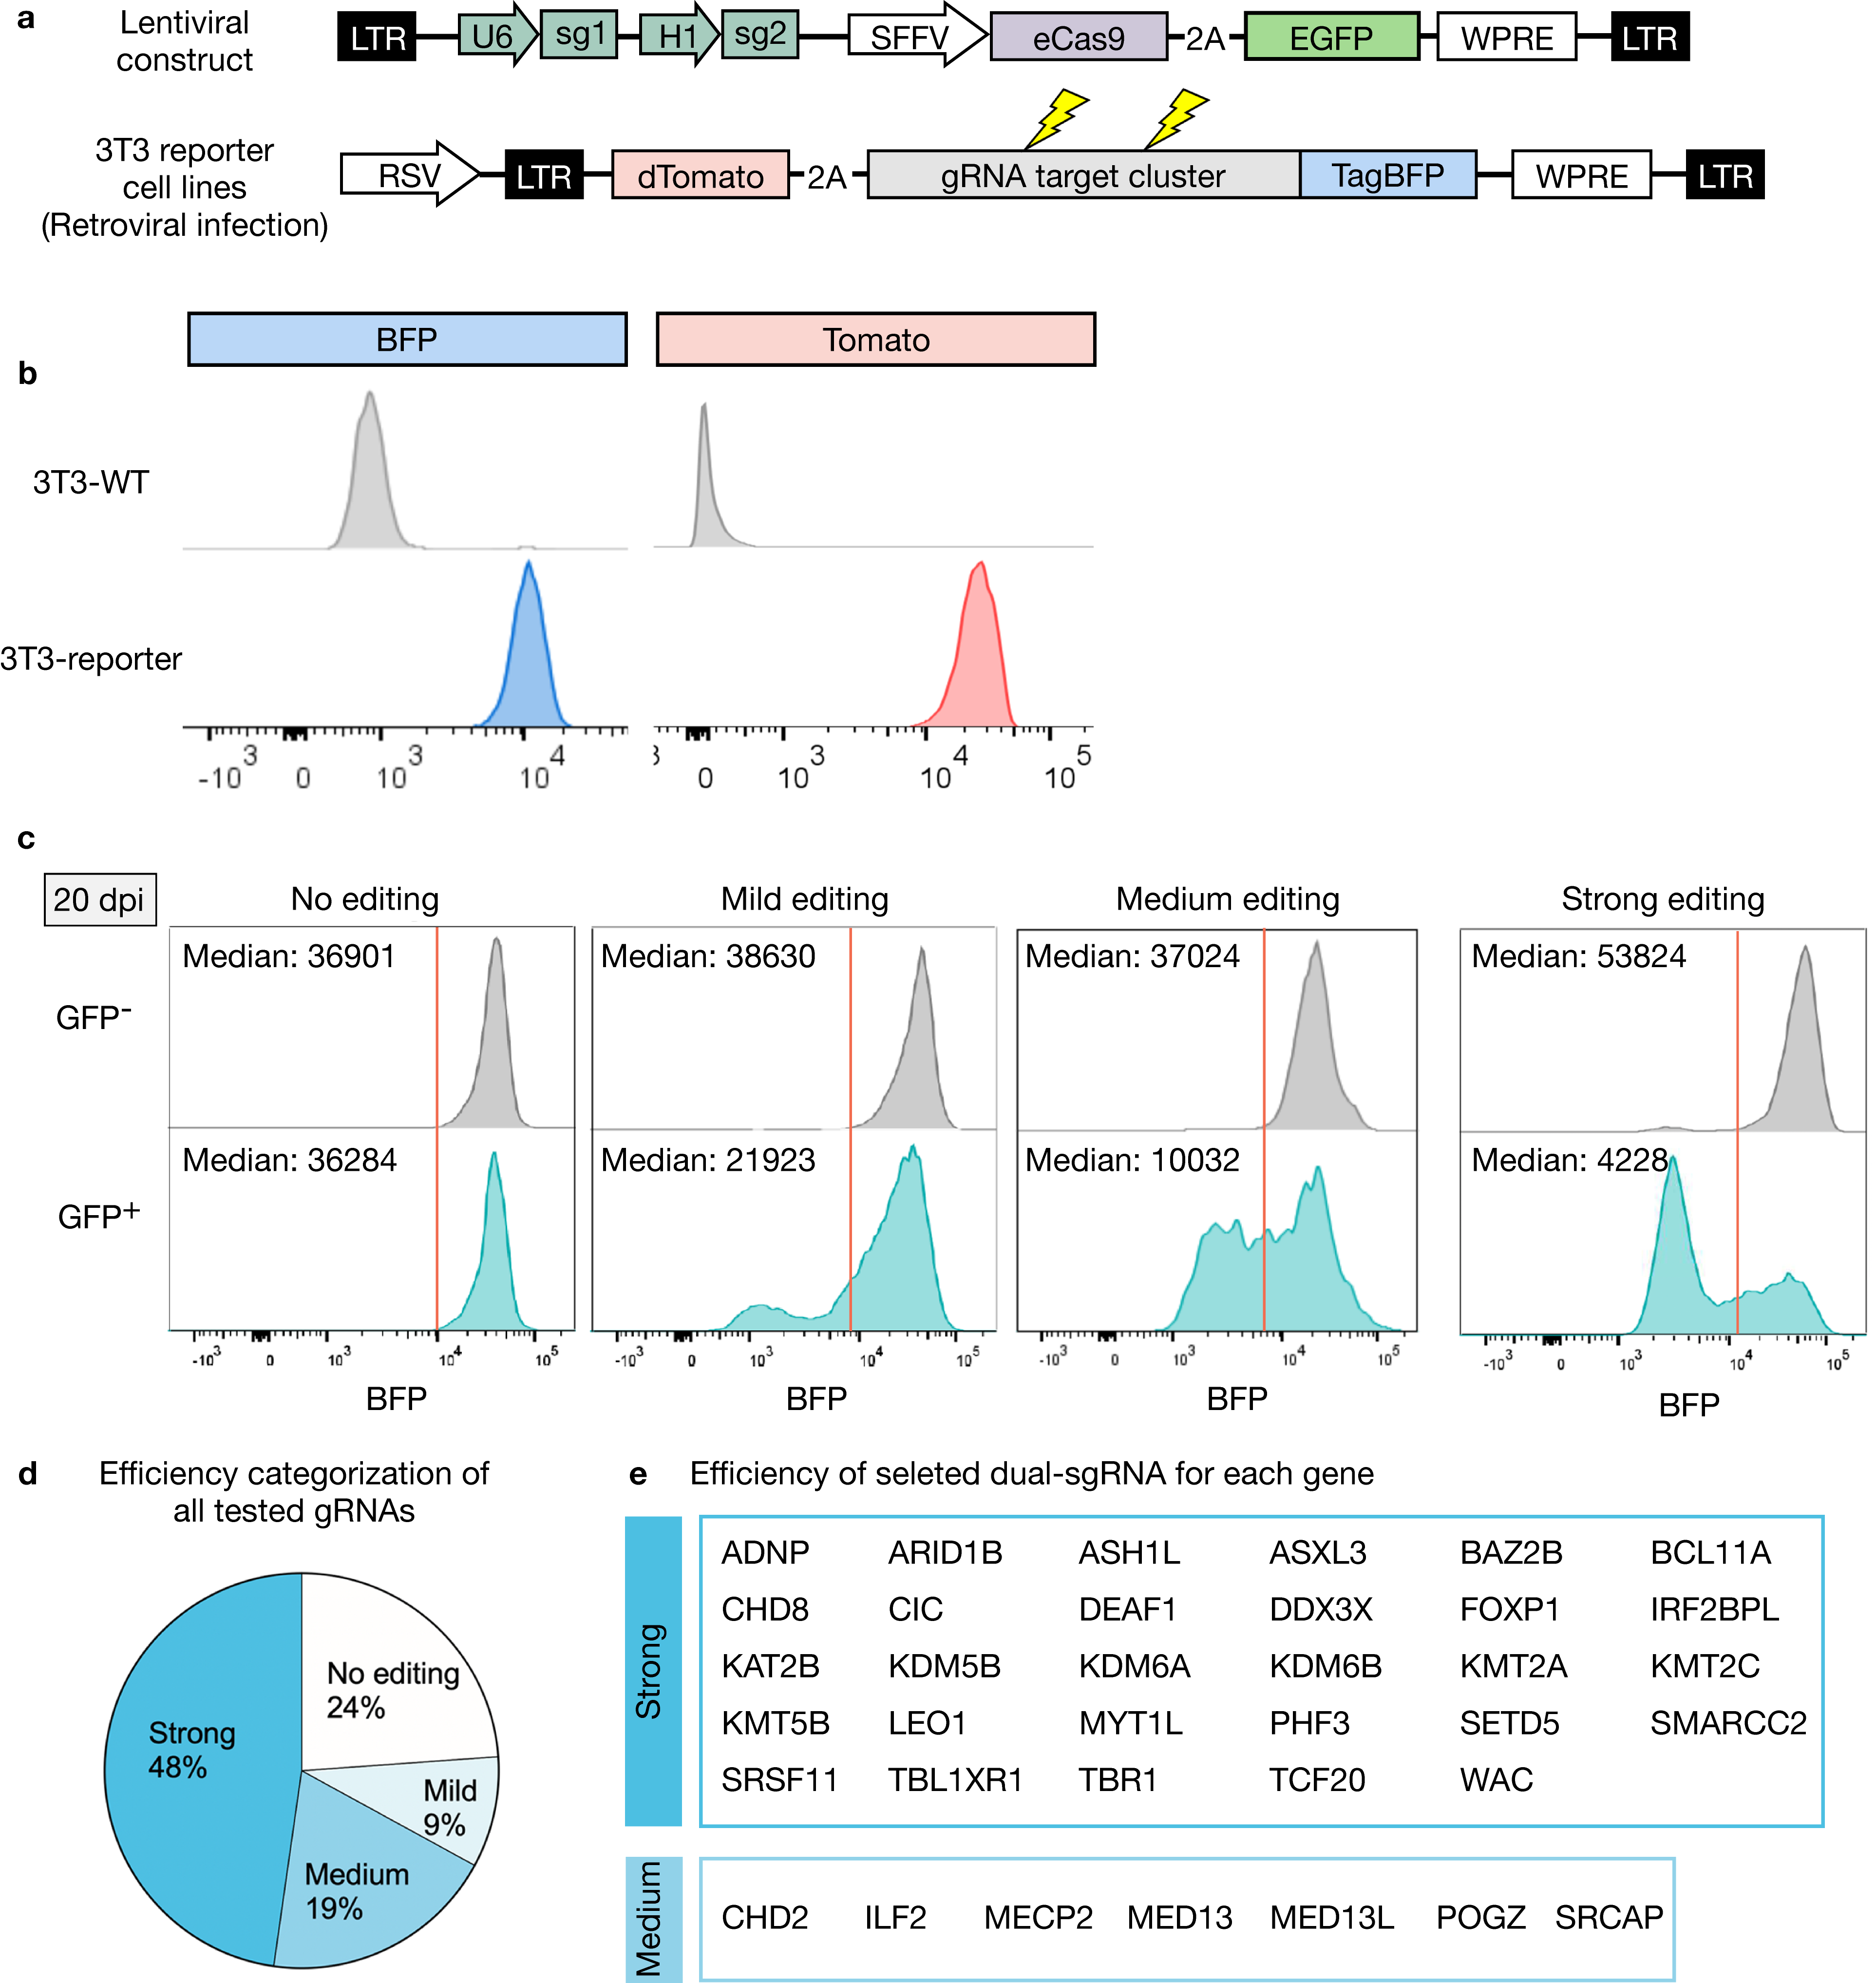
\includegraphics[width=\textwidth]{figures/pando/Figure_S1}
    \label{fig:regS1}
\end{figure}

\clearpage

\begin{figure}[t!]
    \centering
    \caption{\textbf{Supplemental analysis of cerebral organoid developmental multiome data.} a, Phase contrast (until day 15) and bright field (day 31-60) showing examples of different stages of organoid development for four different stem cell lines. Images are representative for 96 organoids per line. Scale bar is 200 $\mu$m. b, Schematic of the experimental design and data integration strategy. c, Histogram of scRNA-seq and scATAC-seq quality control metrics. d, Histograms showing assignment log likelihoods for demultiplexing based on single nucleotide variants. e, Bar plot of number of cells for each timepoint (top) and stacked barplot showing proportion of cell lines (bottom) at different time points. f, Distribution of iPSC lines on the UMAP embedding. g, Bar plots showing number matched and unmatched cells during MCMF bipartite matching. h, Histogram showing the number of cells per metacell for each cell line. i, Box plots showing correlation between gene expression and gene activity metrics for two multiome experiments and the integrated metacells (n=477 genes). j, Box plots showing correlation split by stage (n=3527 genes). Genes >95\% confidence intervals of correlation to permuted background are colored in yellow. Box center represents the median, boxes indicate 25\%-75\% interquantile range and whiskers 1.5 * interquantile range. k, Immunohistochemical staining for progenitor cells (SOX2, orange and GLI3, purple) and neurons (TUJ1, green) for 2 month old organoids of four cell lines. DAPI is shown in cyan. Scale bar: 200 $\mu$m. l, UMAP embedding colored by marker gene expression (log(transcript counts per 10k+1)). The range of values is indicated for each plot. m, Hierarchical clustering of pseudotemporal bins. Top bars show stage and proportion of time points per bin. Heatmap shows min-max scaled mean accessibility (tf-idf normalized fragment counts) of stage-specific peak clusters for each pseudotime bin. Representative GREAT enrichments are shown for each stage.}
\end{figure}


\begin{figure}[h!]
    \centering
	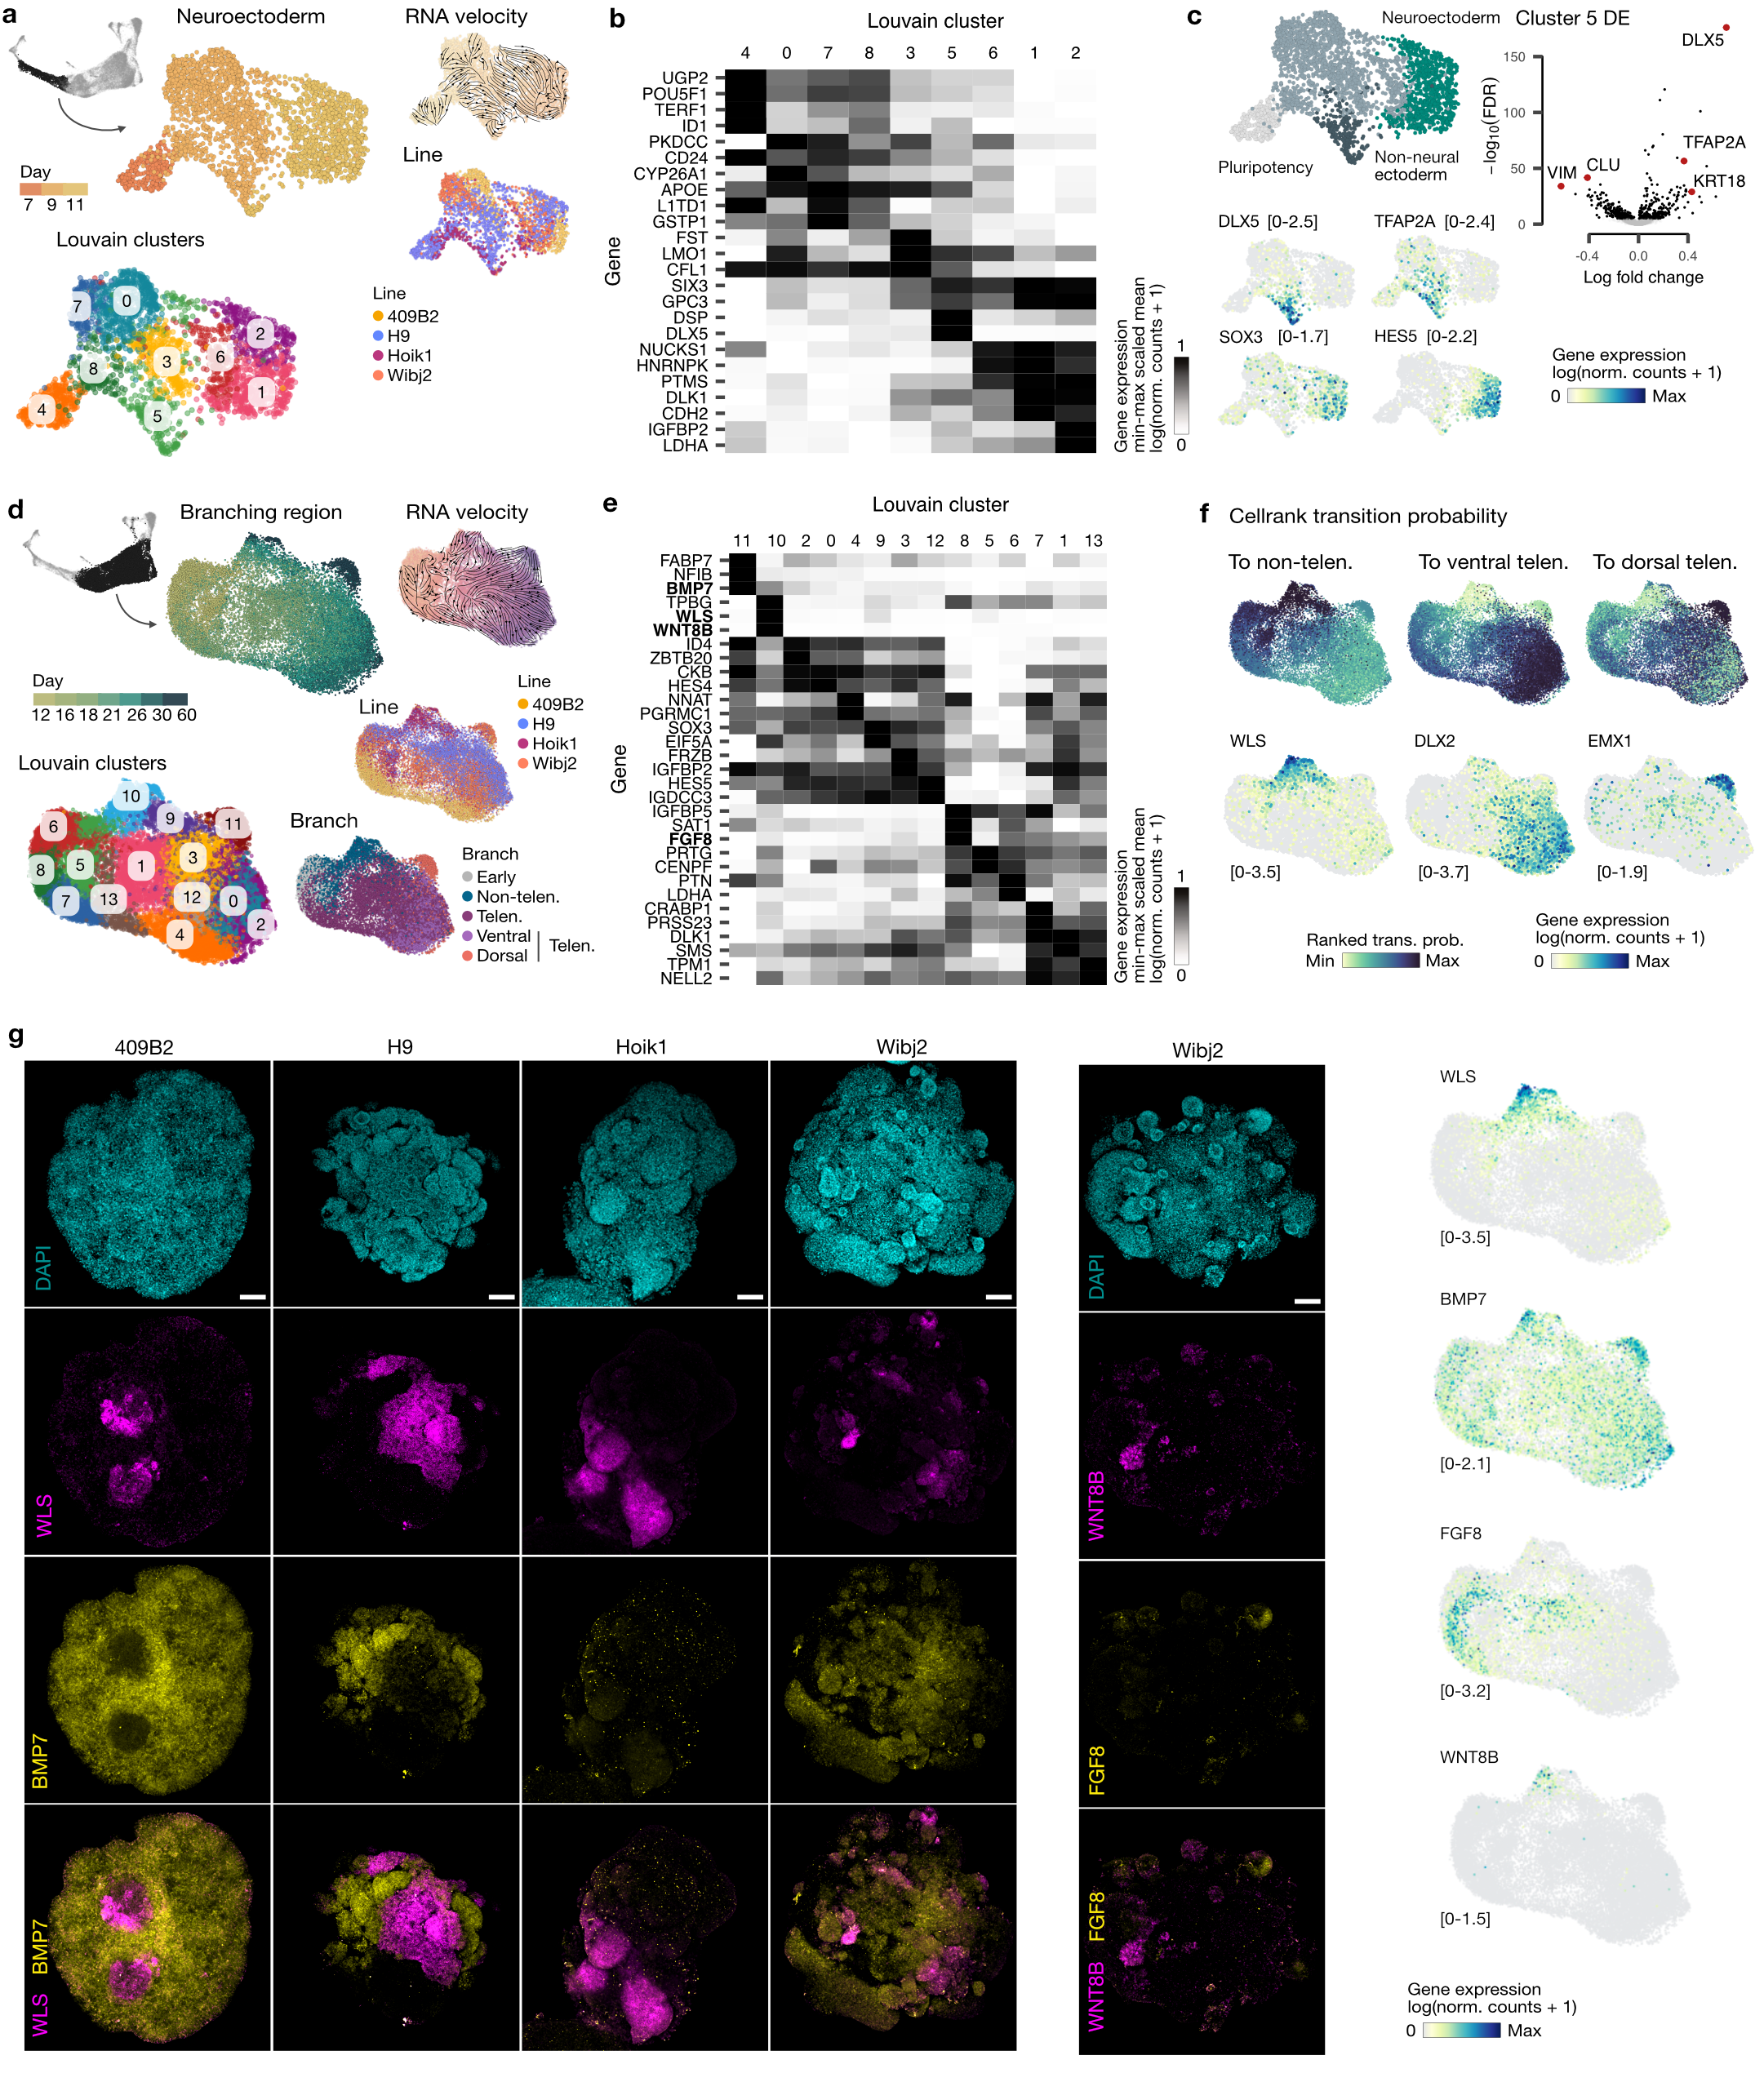
\includegraphics[width=\textwidth]{figures/pando/Figure_S2}
    \label{fig:regS2}
    \caption{\textbf{Heterogeneity analysis in different stages of organoid development.} a,d, UMAP embedding of a subset of the organoid trajectory surrounding neuroectoderm cells (a) and the branching window (d) colored by time point, velocity pseudotime, cell line, branch prediction and lovain clusters. b,e, Heatmap showing mean min-max scaled expression (log(transcript counts per 10k + 1)) of cluster markers. c, UMAP embedding colored by cluster identities, expression patterns of cluster markers. Volcano plot shows differentially expressed (DE) genes of cluster 5 relative to other clusters. f, UMAP embedding colored by rank-transformed CellRank transition probability to non-telencephalon, ventral telencephalon and dorsal telencephalon and colored by expression of selected transcription factors. g, Whole-mount HCR in situ hybridizations of day 18 organoids and UMAP embedding colored by expression of targets. Stainings were performed on 2-3 organoids per cell line and representative images were shown. Scale bar: 100 $\mu$m. The range of expression values is indicated for each feature plot.}
\end{figure}


\begin{figure}[h!]
    \centering
	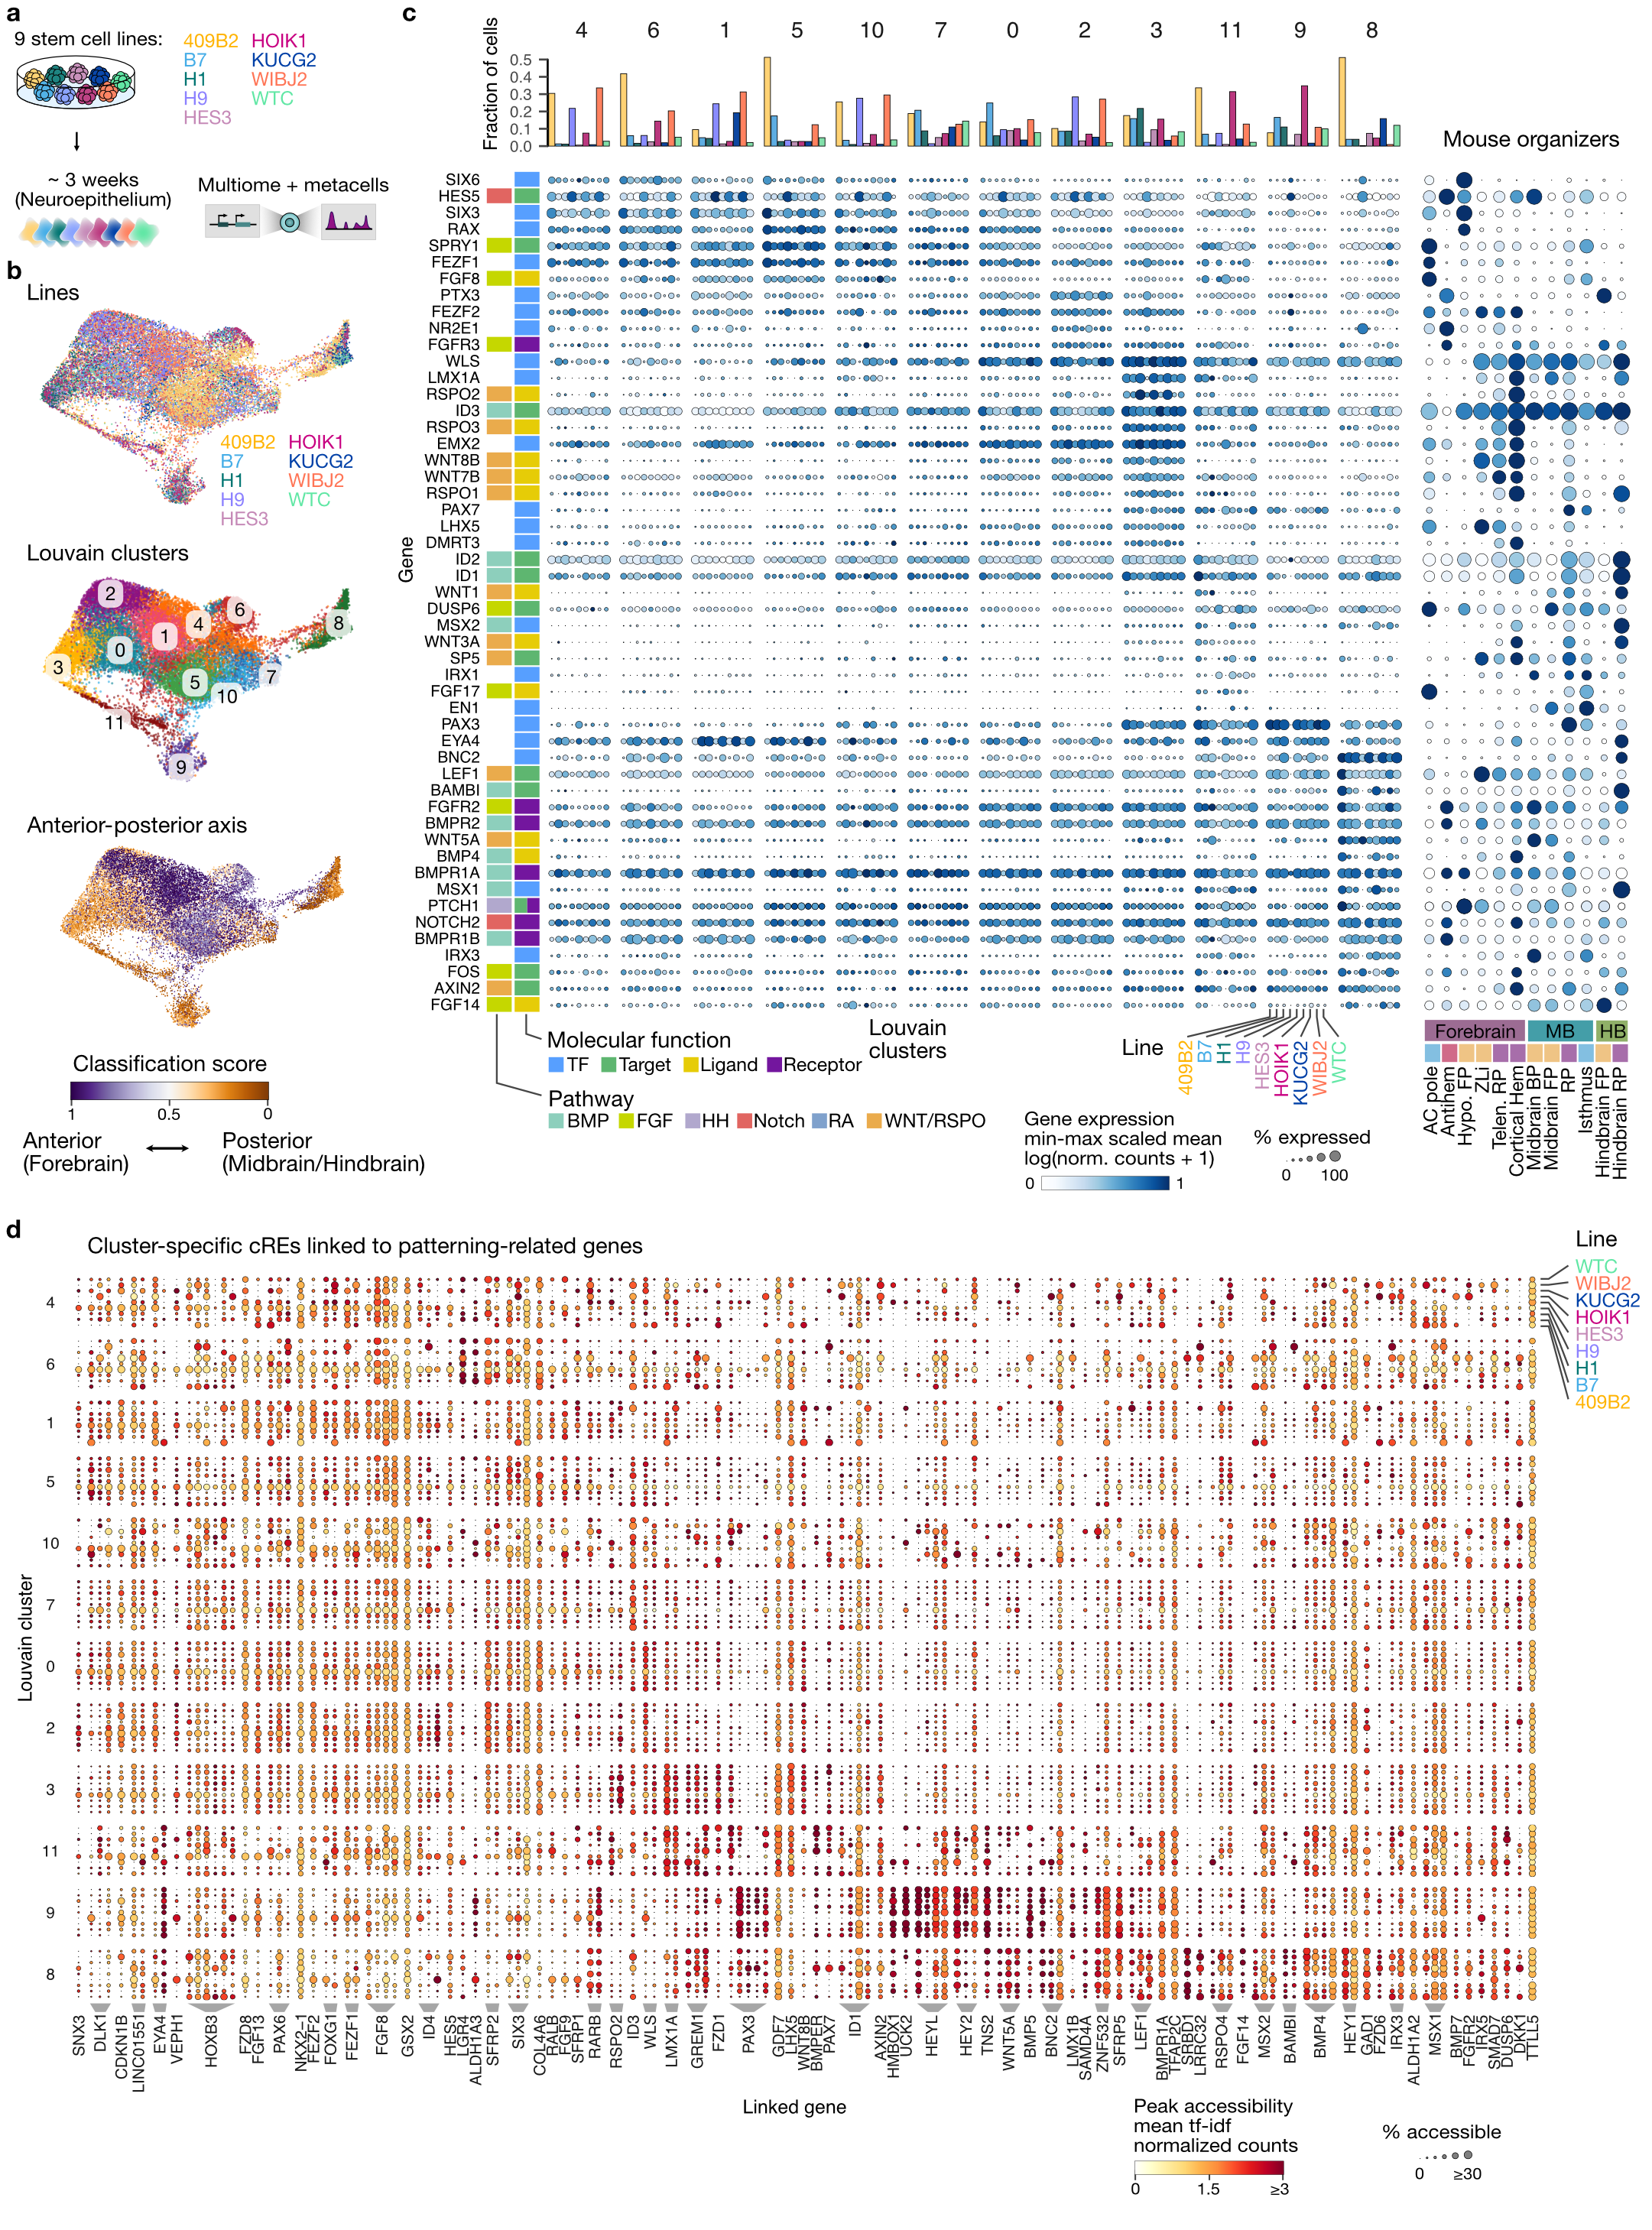
\includegraphics[width=\textwidth]{figures/pando/Figure_S3}
    \label{fig:regS3}
\end{figure}

\begin{figure}[t!]
    \centering
    \caption{\textbf{Signaling transcriptome and regulatory element landscape of the organoid neuroepithelium from 9 stem cell lines.} a, Schematic of the experimental setup. Multiome quantification was performed on organoids in the neuroepithelial stage (~3 weeks) from a total of 9 stem cell lines. The data was combined with the data from the same stage in the early time course. b, UMAP embedding colored by cell line, louvain clusters and anterior-posterior axis (forebrain versus non-forebrain) classification score. c, Bar plots (top) showing fraction of cells per cell line in each cluster. Dotplot (left) showing min-max scaled expression (log(transcript counts per 10k + 1))(color) and proportion of expressing cells (dot size) for transcription factors (TFs) and genes from different signaling pathways in clusters of 3 week old organoid data set split by cell line. All genes are annotated as TF, receptor, ligand, or TF target and if applicable, colored by the related signaling pathway. Dotplot (right) showing expression (color) and proportion of expressing cells (dot size) for the same genes of Figure S3.3d in mouse developing brain organizer cells of different brain regions (\cite{la_manno_molecular_2021}). d, Dot plot showing cluster-specific cis regulatory elements (CREs) linked to patterning genes split by different cell lines. Color and size indicate peak accessibility (if-idf normalized fragment counts) and proportion of expressing cells, respectively.}
\end{figure}

\clearpage

\begin{figure}[h!]
    \centering
	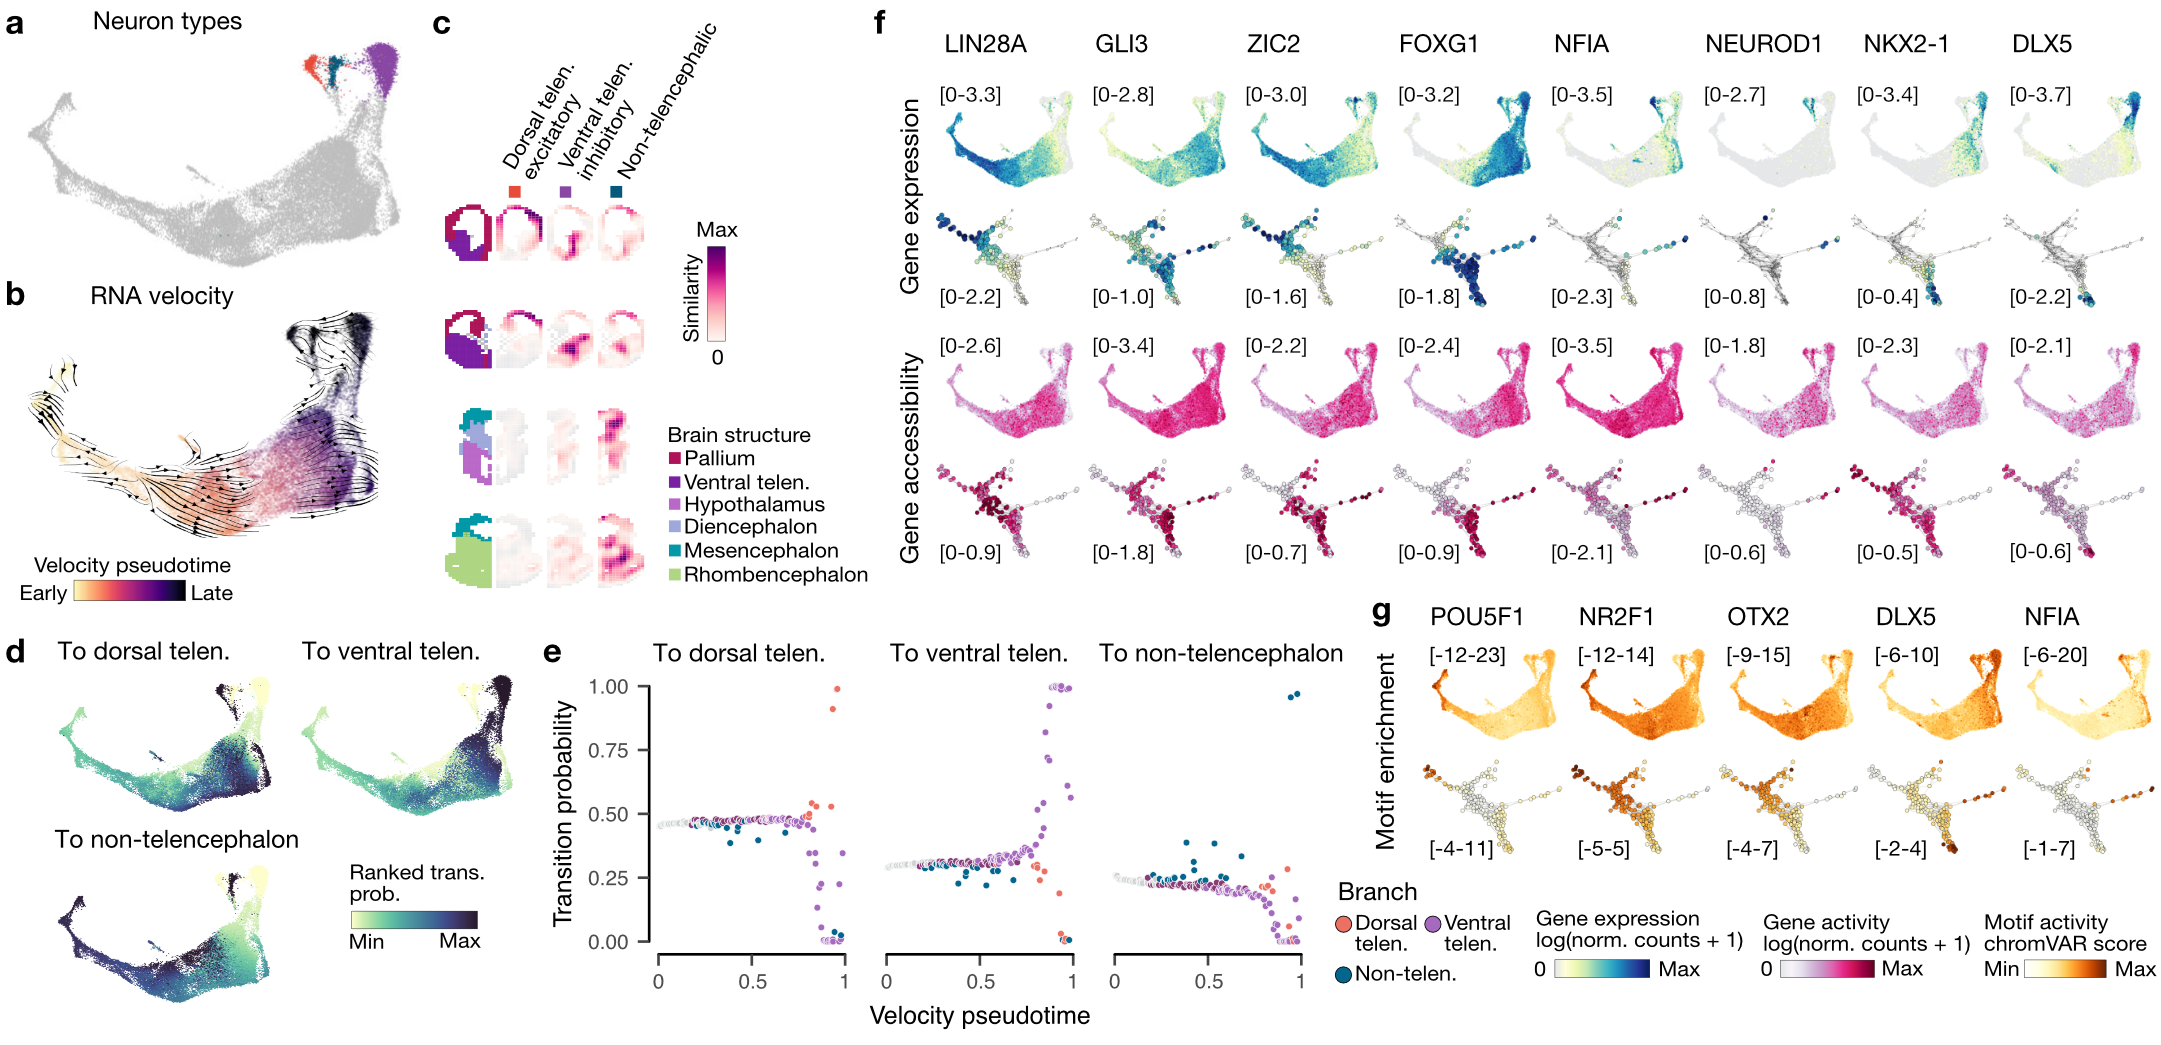
\includegraphics[width=\textwidth]{figures/pando/Figure_S4}
    \caption{\textbf{Trajectory reconstruction in the multi-omic developmental atlas.} a, Time course UMAP embedding colored by neuron types. b, Time course UMAP embedding colored by RNA velocity pseudotime. c, VoxHunt plots showing expression similarity of neuron subtypes in cerebral organoids to voxels in five example sections of the developing mouse brain (embryonic day 13.5),  as well as the structural annotation of the sections. d, UMAP embedding colored by ranked transition probabilities. e, Scatter plot showing mean transition probabilities as computed by CellRank versus velocity pseudotime. Each dot represents one high-resolution cluster. f, UMAP embedding of the integrated time course and graph embedding colored by gene expression (log(transcript counts per 10k +1)) (top) and gene activity (log(fragment counts per 10k +1))  (bottom) for selected marker genes. g, UMAP and graph representation colored by transcription factor motif enrichment z-score calculated with chromVAR (\cite{schep_chromvar_2017}) for selected motifs. The range of values is indicated for each feature plot.}
    \label{fig:regS4}
\end{figure}



\begin{figure}[h!]
    \centering
	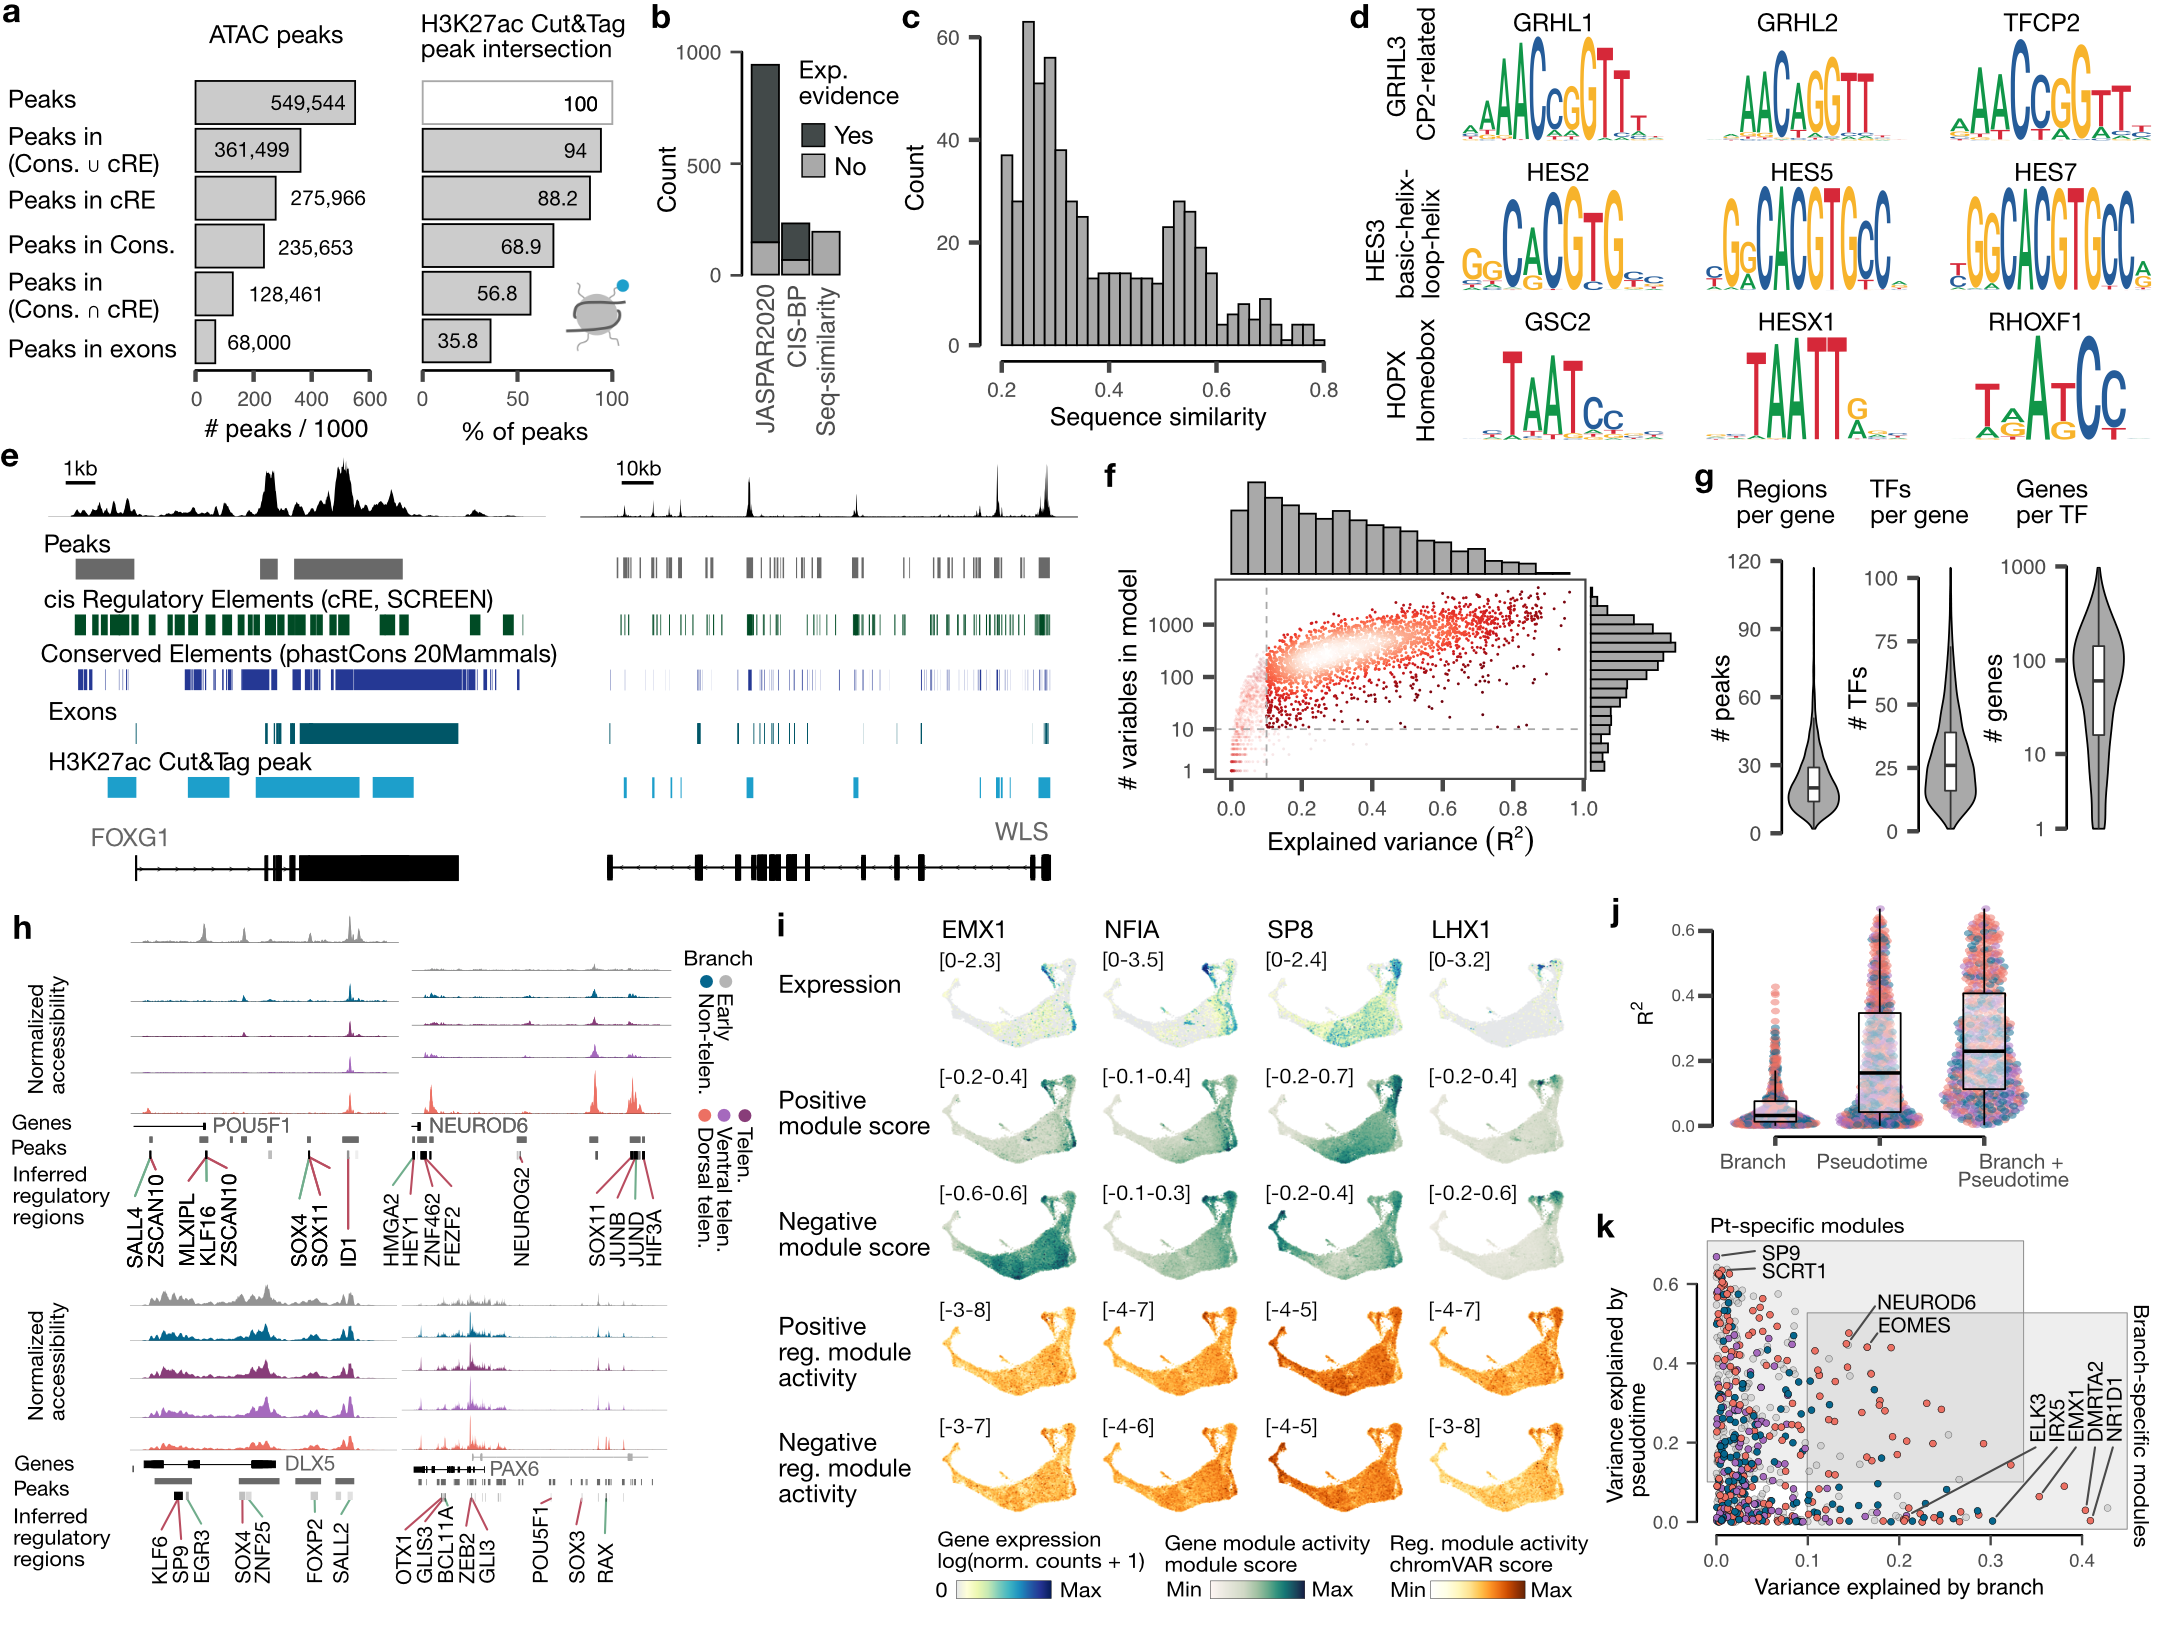
\includegraphics[width=\textwidth]{figures/pando/Figure_S5}
    \label{fig:regS5}
    \caption{\textbf{Gene regulatory network features of cerebral organoid development.} a, Numbers of chromatin access peaks and percentage of H3K27ac-marked peaks accessible at day 18-23 (>5\% detection) intersecting with non-protein coding conserved regions (Cons.), candidate cis regulatory regions (CRE), or exons (left). b, Representative loci showing chromatin access (top) overlaying peak, CRE, conserved elements, and exon coordinates. c, Barplot showing the number of motifs used in GRN construction from two curated databases (JASPAR, CIS-BP), and motifs assigned through amino acid sequence similarity. d, Examples of 3 TFs with no motif annotation that were assigned motifs based on sequence similarity. e, Loci for two exemplary genes (FOXG1, WLS) showing average chromatin access signal tracks, accessible peaks, CREs, conserved elements, exons and H3K27ac Cut\&Tag peaks. f, Scatter plot and histograms show explained variance (x) versus number of variables (y) of models for GRN construction. g, Violin plots show the distribution of peaks (left, n=2535 target genes) and TFs per gene (middle, n=2535 target genes), and number of genes per TF (right, n=720 TFs). h, Representative loci showing average chromatin access signal tracks at different developmental branches overlaying inferred transcription factor binding sites within regulatory regions. i, UMAP representation of time course colored by gene expression (log(transcript counts per 10k + 1)), gene module activity (module score calculated with Seurat) (rows), and regulatory module enrichment z-score (calculated with chromVAR) for representative TFs (columns). The range of values is indicated for each plot. j, Variation of module activity explained by branch, pseudotime, or branch and pseudotime (n=720 TF modules). Box plot center lines represent the median, boxes indicate 25\%-75\% interquantile range and whiskers 1.5 * interquantile range. k, Branch and pseudotime specific TF modules. Colors represent the branch with highest average module activity. TFs without experimentally validated motif are shown in gray. }
\end{figure}


\begin{figure}[h!]
    \centering
	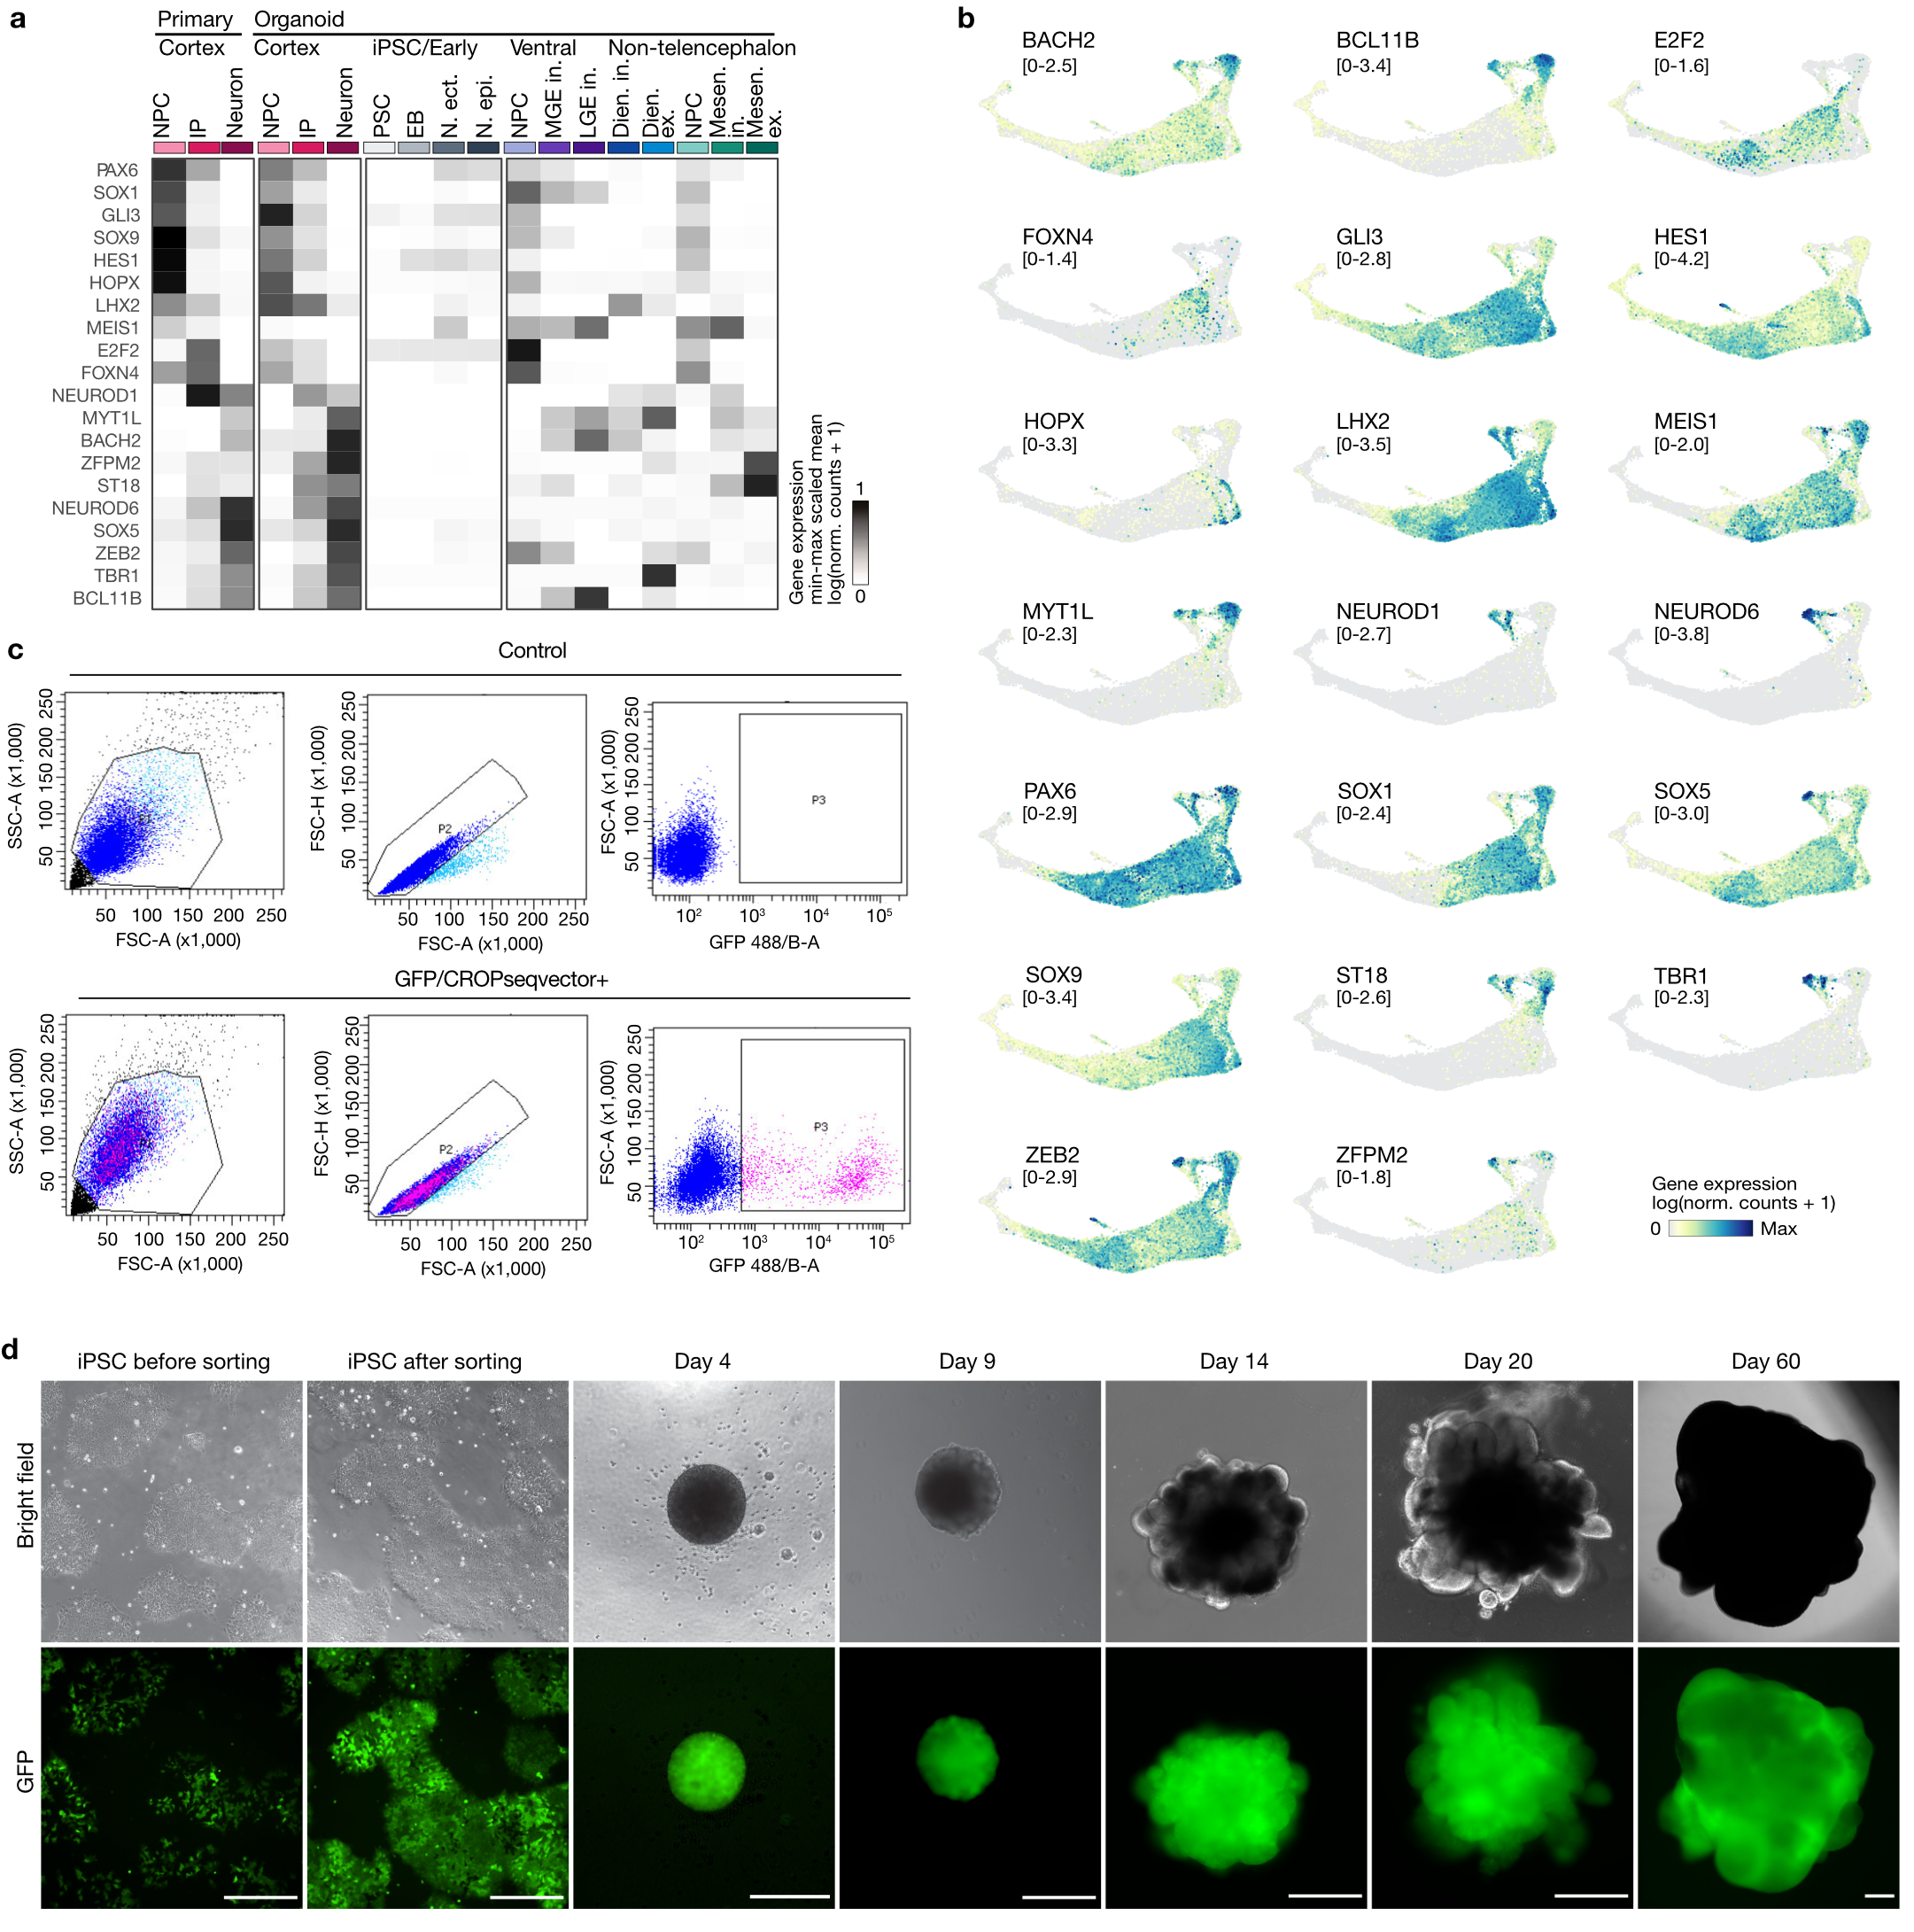
\includegraphics[width=\textwidth]{figures/pando/Figure_S6}
    \label{fig:regS6}
    \caption{\textbf{Target selection and experimental details for the single-cell \textit{in organoid} perturbation experiment.} a, Min-max scaled mean expression (log(transcript counts per 10k + 1)) of genes targeted in the single-cell genomic perturbation experiment in neuronal progenitors (NP), intermediate progenitors (IP) and neurons in the primary human and organoid developing cortex, as well as in induced pluripotent stem cells (IPSC), the embryoid body (EB), ventral telencephalic NPCs, inhibitory neurons of the medial ganglionic eminence (MGE in.), lateral ganglionic eminence (LGE in.), non-telencephalic NPCs, diencephalic excitatory neurons (Dien. ex.) and inhibitory neurons (Dien. in.) and mesencephalic excitatory neurons (Mesen. ex.) and inhibitory neurons (Mesen. in.). b, UMAP embedding colored by the expression of all targeted genes. The range of expression values is indicated for each feature plot. c, Exemplary Fluorescence-activated cell sorting plots of the sorting scheme used to isolate CROP-seq vector positive induced pluripotent stem cells (iPSCs). d, Phase contrast and CROP-seq vector positive (GFP) imaging during cerebral organoid development. Images are representative for 48 imaged organoids. Scale Bar is 500 $\mu$m.}
\end{figure}


\begin{figure}[h!]
    \centering
	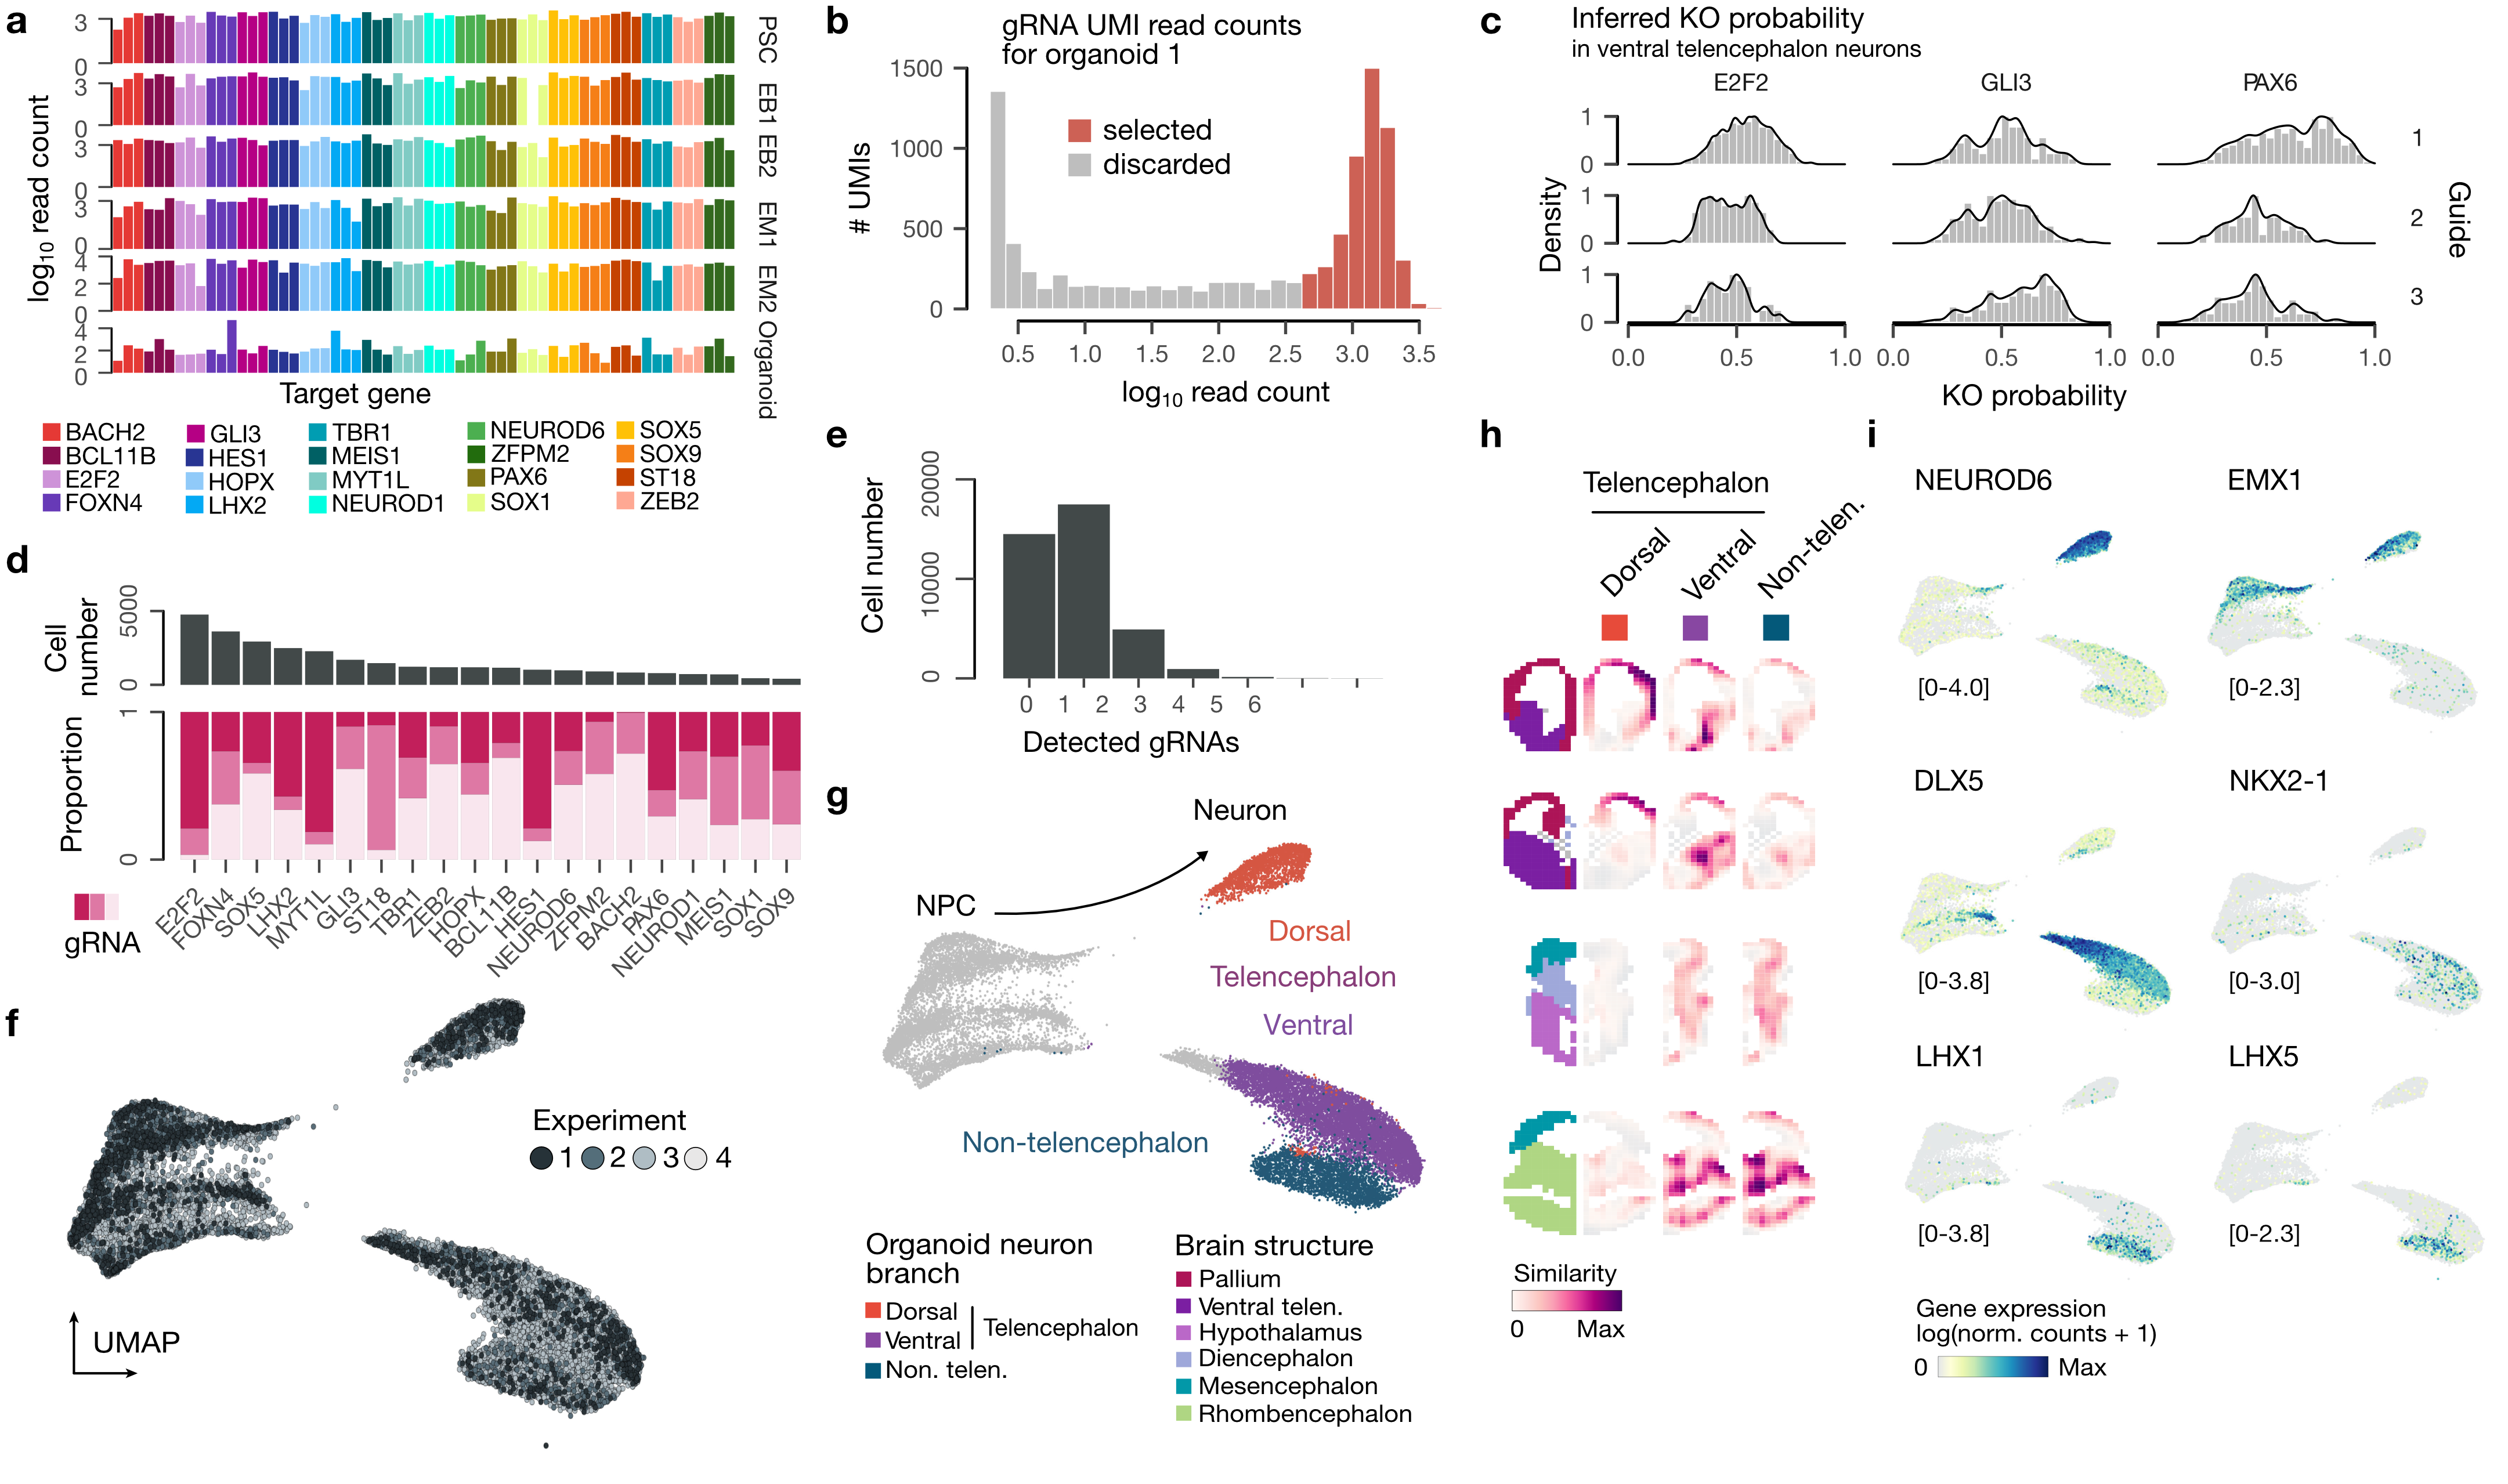
\includegraphics[width=\textwidth]{figures/pando/Figure_S7}
    \label{fig:regS7}
    \caption{\textbf{Guide detection and cell type annotation in the single-cell perturbation experiment in organoids.} a, Barplot showing number of cells with detected guide RNA (gRNA) for each targeted gene and stacked barplot showing the distribution of the different gRNAs targeting the same gene. b, Histogram showing the distribution of read counts for gRNA UMIs after amplicon sequencing for one organoid. UMIs marked in red were selected for downstream analyses. c, Density histograms showing the distribution of inferred KO probabilities for gRNAs of 3 different target genes. d, Barplot showing cell number and proportion of gRNAs for all target genes. e, Barplot showing the number of guides detected in sequenced cells. f, UMAP embedding with cells colored based on experiment. g, UMAP embedding colored by annotated neuron subtypes. h, VoxHunt plots showing expression similarity of neuron subtypes in cerebral organoids to voxels in five example sections of the developing mouse brain (embryonic day 13.5), as well as the structural annotation of the sections (left). i, UMAP embedding colored by expression (log(transcript counts per 10k + 1)) of non-telencephalic (top), ventral (middle) and dorsal (bottom) neuron markers. The range of expression values is indicated for each feature plot.}
\end{figure}




\begin{figure}[h!]
    \centering
	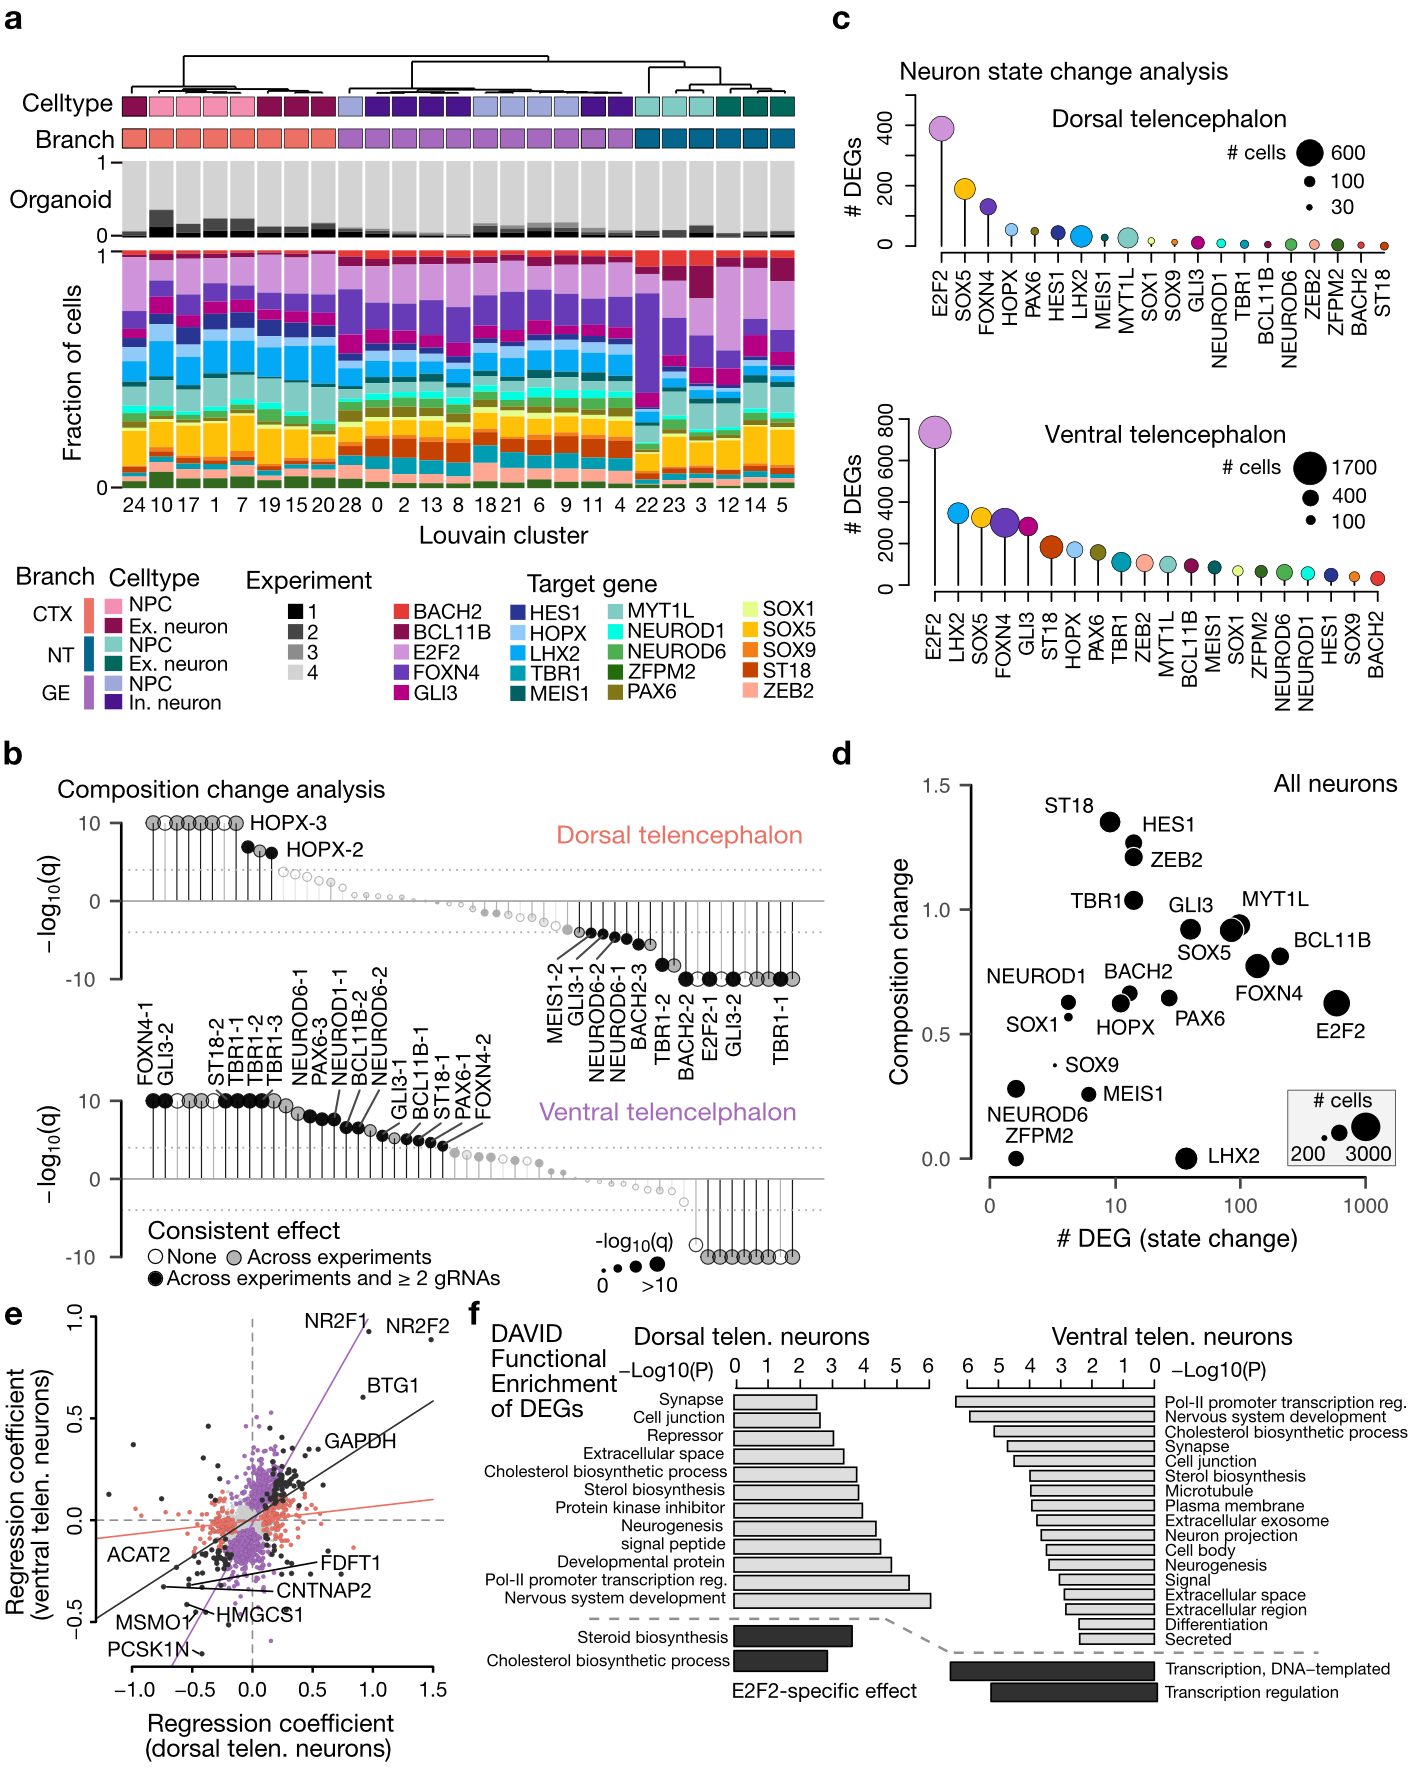
\includegraphics[width=\textwidth]{figures/pando/Figure_S8}
    \label{fig:regS8}
\end{figure}

\begin{figure}[h!]
    \centering
    \caption{\textbf{Composition and expression changes after CRISPR-Cas9 perturbations in mosaic brain organoids.} a, Hierarchical clustering of Louvain clusters based on the composition of gRNAs targeting different genes. Cell type and branch annotations are shown as side bars. Compositions of organoids and composition of cells with gRNAs targeting different genes are shown below as stacked bar plots. b, Lollipop plot showing the impact of each gRNA on cell type abundance in dorsal and ventral telencephalic neurons. c, Lollipop plots showing number of differentially expressed genes (DEG) for targeted genes in the dorsal and ventral telencephalic neurons. d, Differential gene expression analysis was performed to identify potential effects on cell state. Plot shows the effect of cell composition change and the number of differentially expressed genes (DEGs). P-values were derived using an F-test based ANCOVA.  e, Scatter plot shows expression changes between neurons with E2F2 targeting gRNAs and other neurons in dorsal (x-axis) and ventral (y-axis) telencephalic neurons, with each dot representing one gene. Colors of dots represent the neuron types where differential expression is detected. Lines show the correlation of expression changes in the two neuron types, with DE genes in both types and DE genes in only one type shown separately. f, Examples of functional enrichment for E2F2 DEGs in dorsal and ventral neurons with DAVID. Gray bars show enriched terms of all E2F2 DEGs, and dark bars show enriched terms of DEGs with E2F2-specific effects.}
\end{figure}

\clearpage


\begin{figure}[h!]
    \centering
	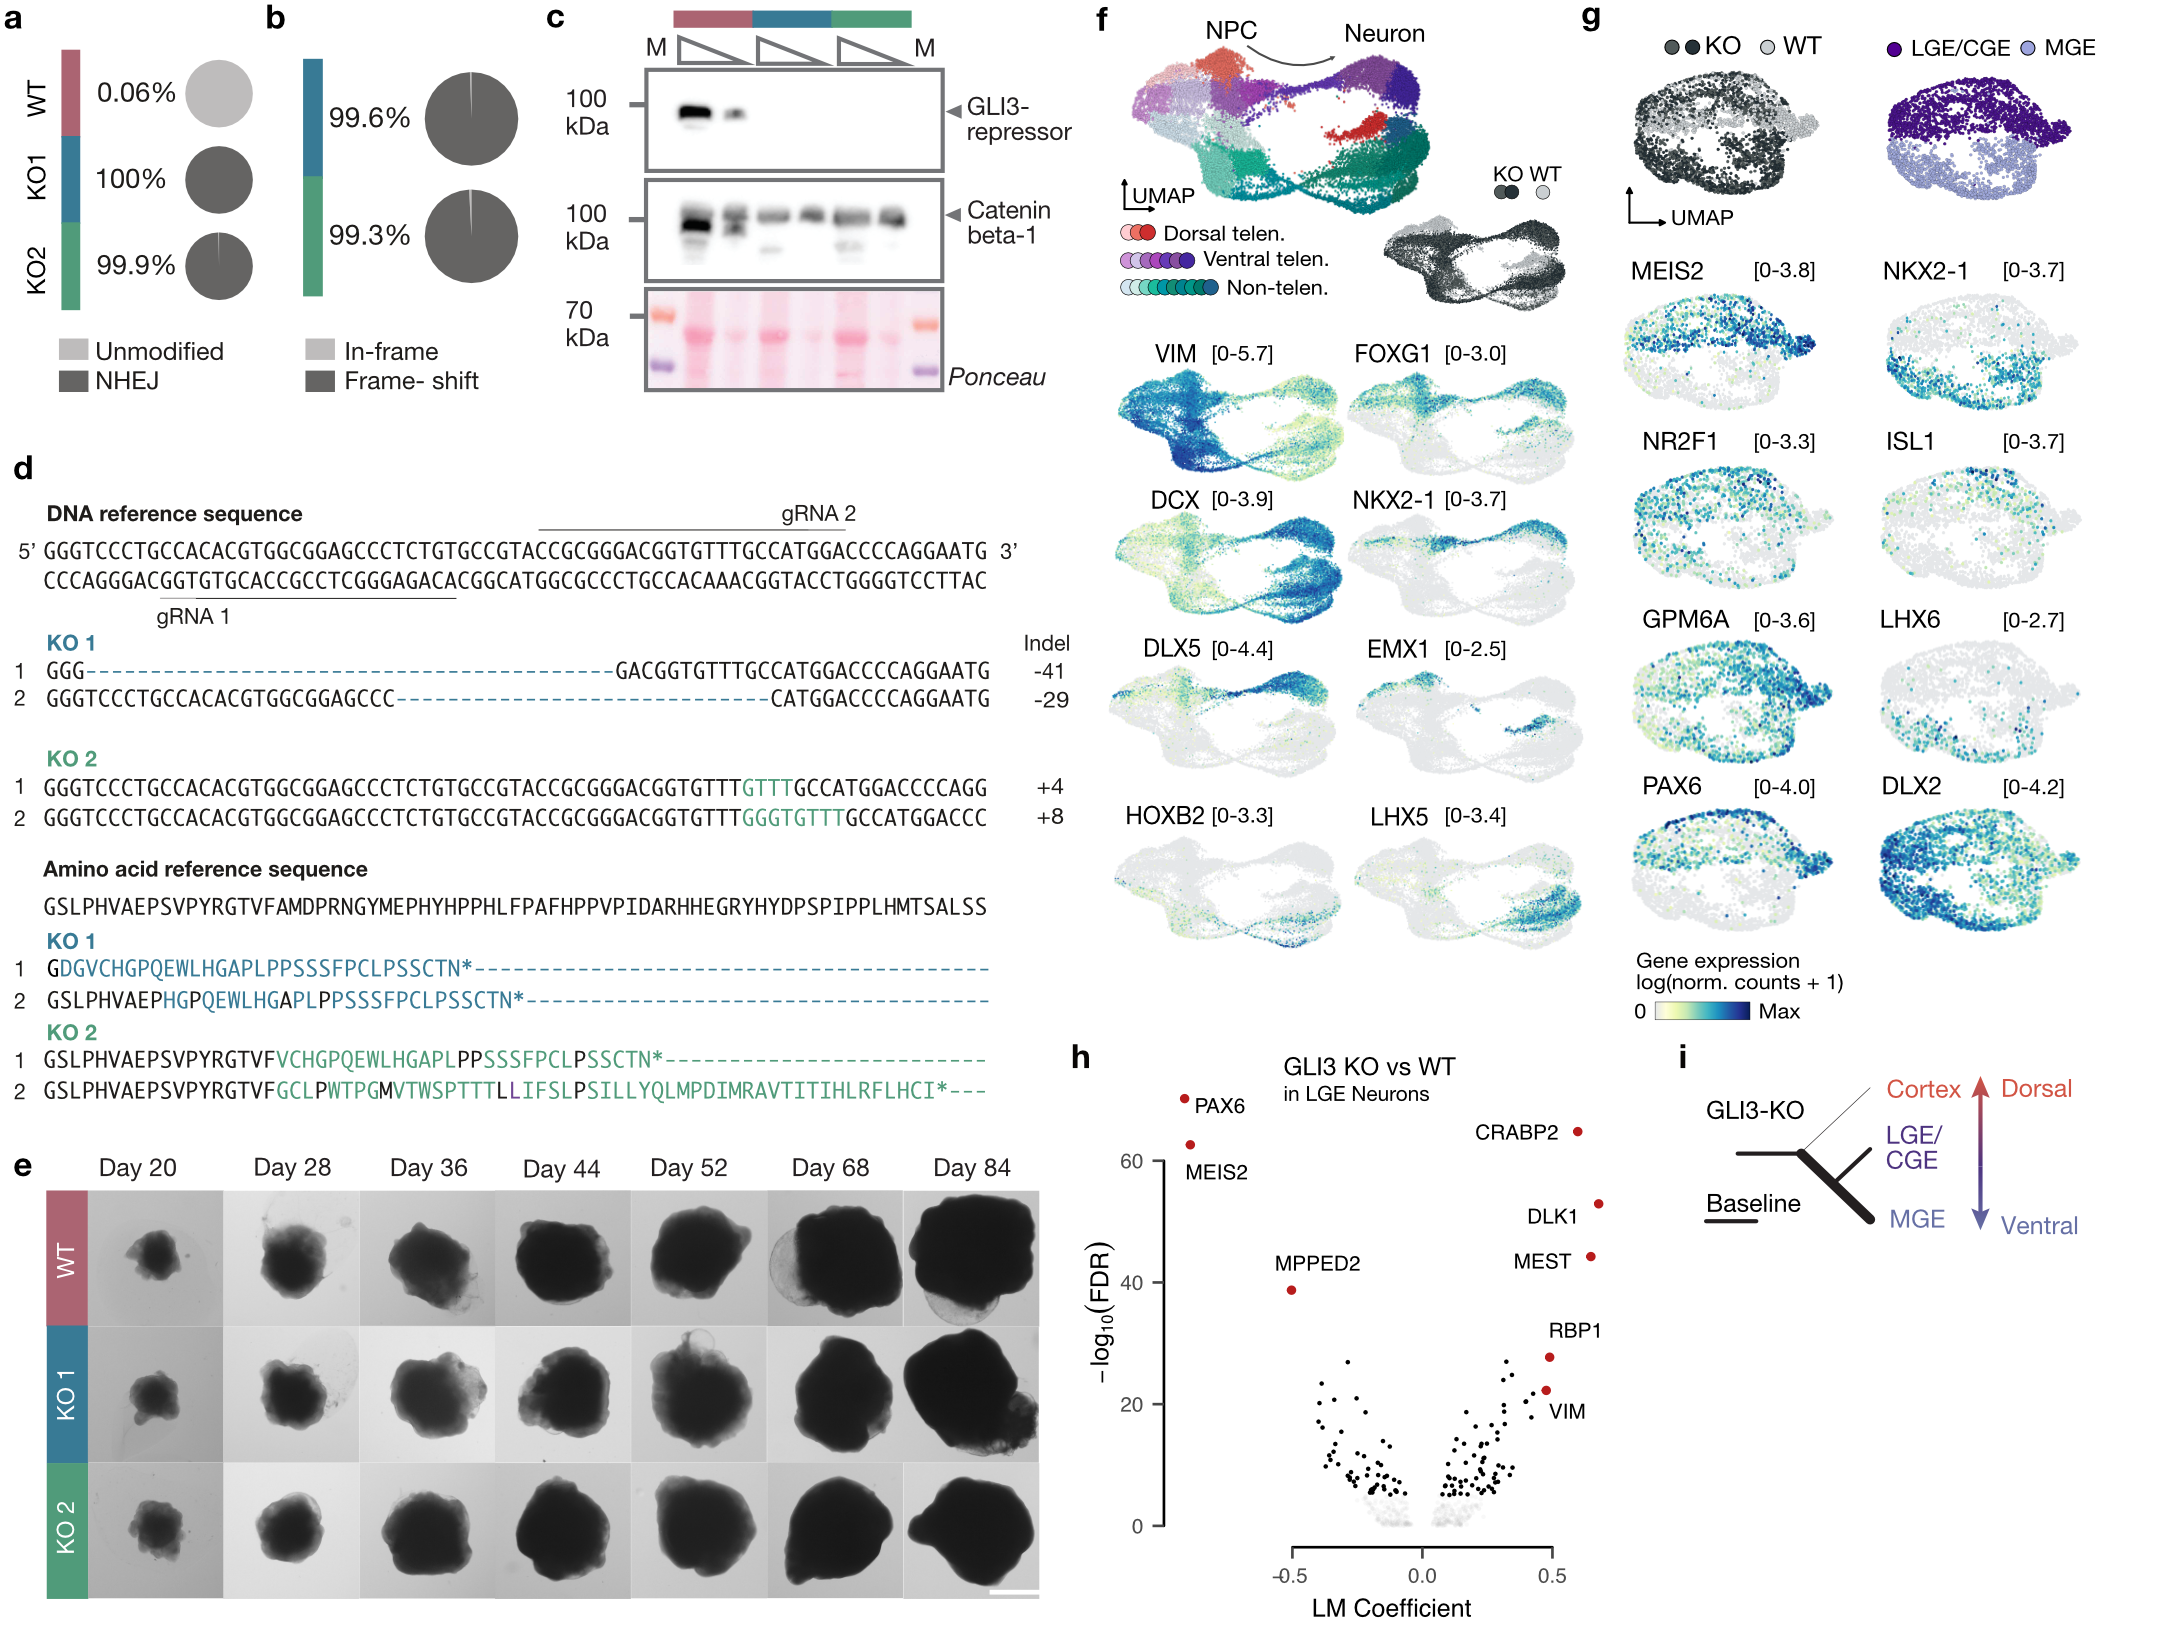
\includegraphics[width=\textwidth]{figures/pando/Figure_S9}
    \label{fig:regS9}
    \caption{\textbf{Characterization of GLI3 knock-out organoids.} Quantification of editing frequency as determined by the percentage and number of sequence reads showing unmodified and modified alleles for the control and both KO cell lines. b, Frequency of frameshift of coding sequence reads as a result of the modifications seen in both KO lines. c, Western blot showing expression of Gli3-repressor (83kDA) in the control cell line. Catenin beta-1 and Ponceau were used as loading control. For western blot source data, see Supplementary Data Figure 3.1. d, Sequences of the coding strand of the different indels of the different KO lines. The reference sequence is corresponding with the control line. The position of the gRNAs with the protospacer adjacent motif (PAM)-sequence is depicted above and underneath the sequence. Reference protein sequence with the protein sequences of each KO line of the altered protein sequences caused by the frame-shift. e, Brightfield images of cerebral organoid development with control and both KO cell lines. Images are representative for 16 imaged organoids per line. Scale bar is 2 mm. f, UMAP embedding showing trajectories from neural progenitor cells (NPCs) to neurons colored by different clusters assigned to branches (dorsal, ventral, and non-telencephalon), with inset colored by genetic condition and feature plots colored by expression (log(transcript counts per 10k + 1)) of cell type markers. g, UMAP embedding of ventral telencephalic GLI3 KO neurons showing medial ganglionic eminence (MGE) and lateral/caudal ganglionic eminence (LGE/CGE) neuronal populations (top). Feature plots show selected marker gene expression on the UMAP embedding. The range of expression values is indicated for each feature plot. h, Volcano plot showing differential expression analysis in LGE neurons for GLI3 WT versus KO cells. i, Schematic of observed effect of GLI3 loss of function on dorsoventral telencephalic fate decisions. }
\end{figure}


\begin{figure}[h!]
    \centering
	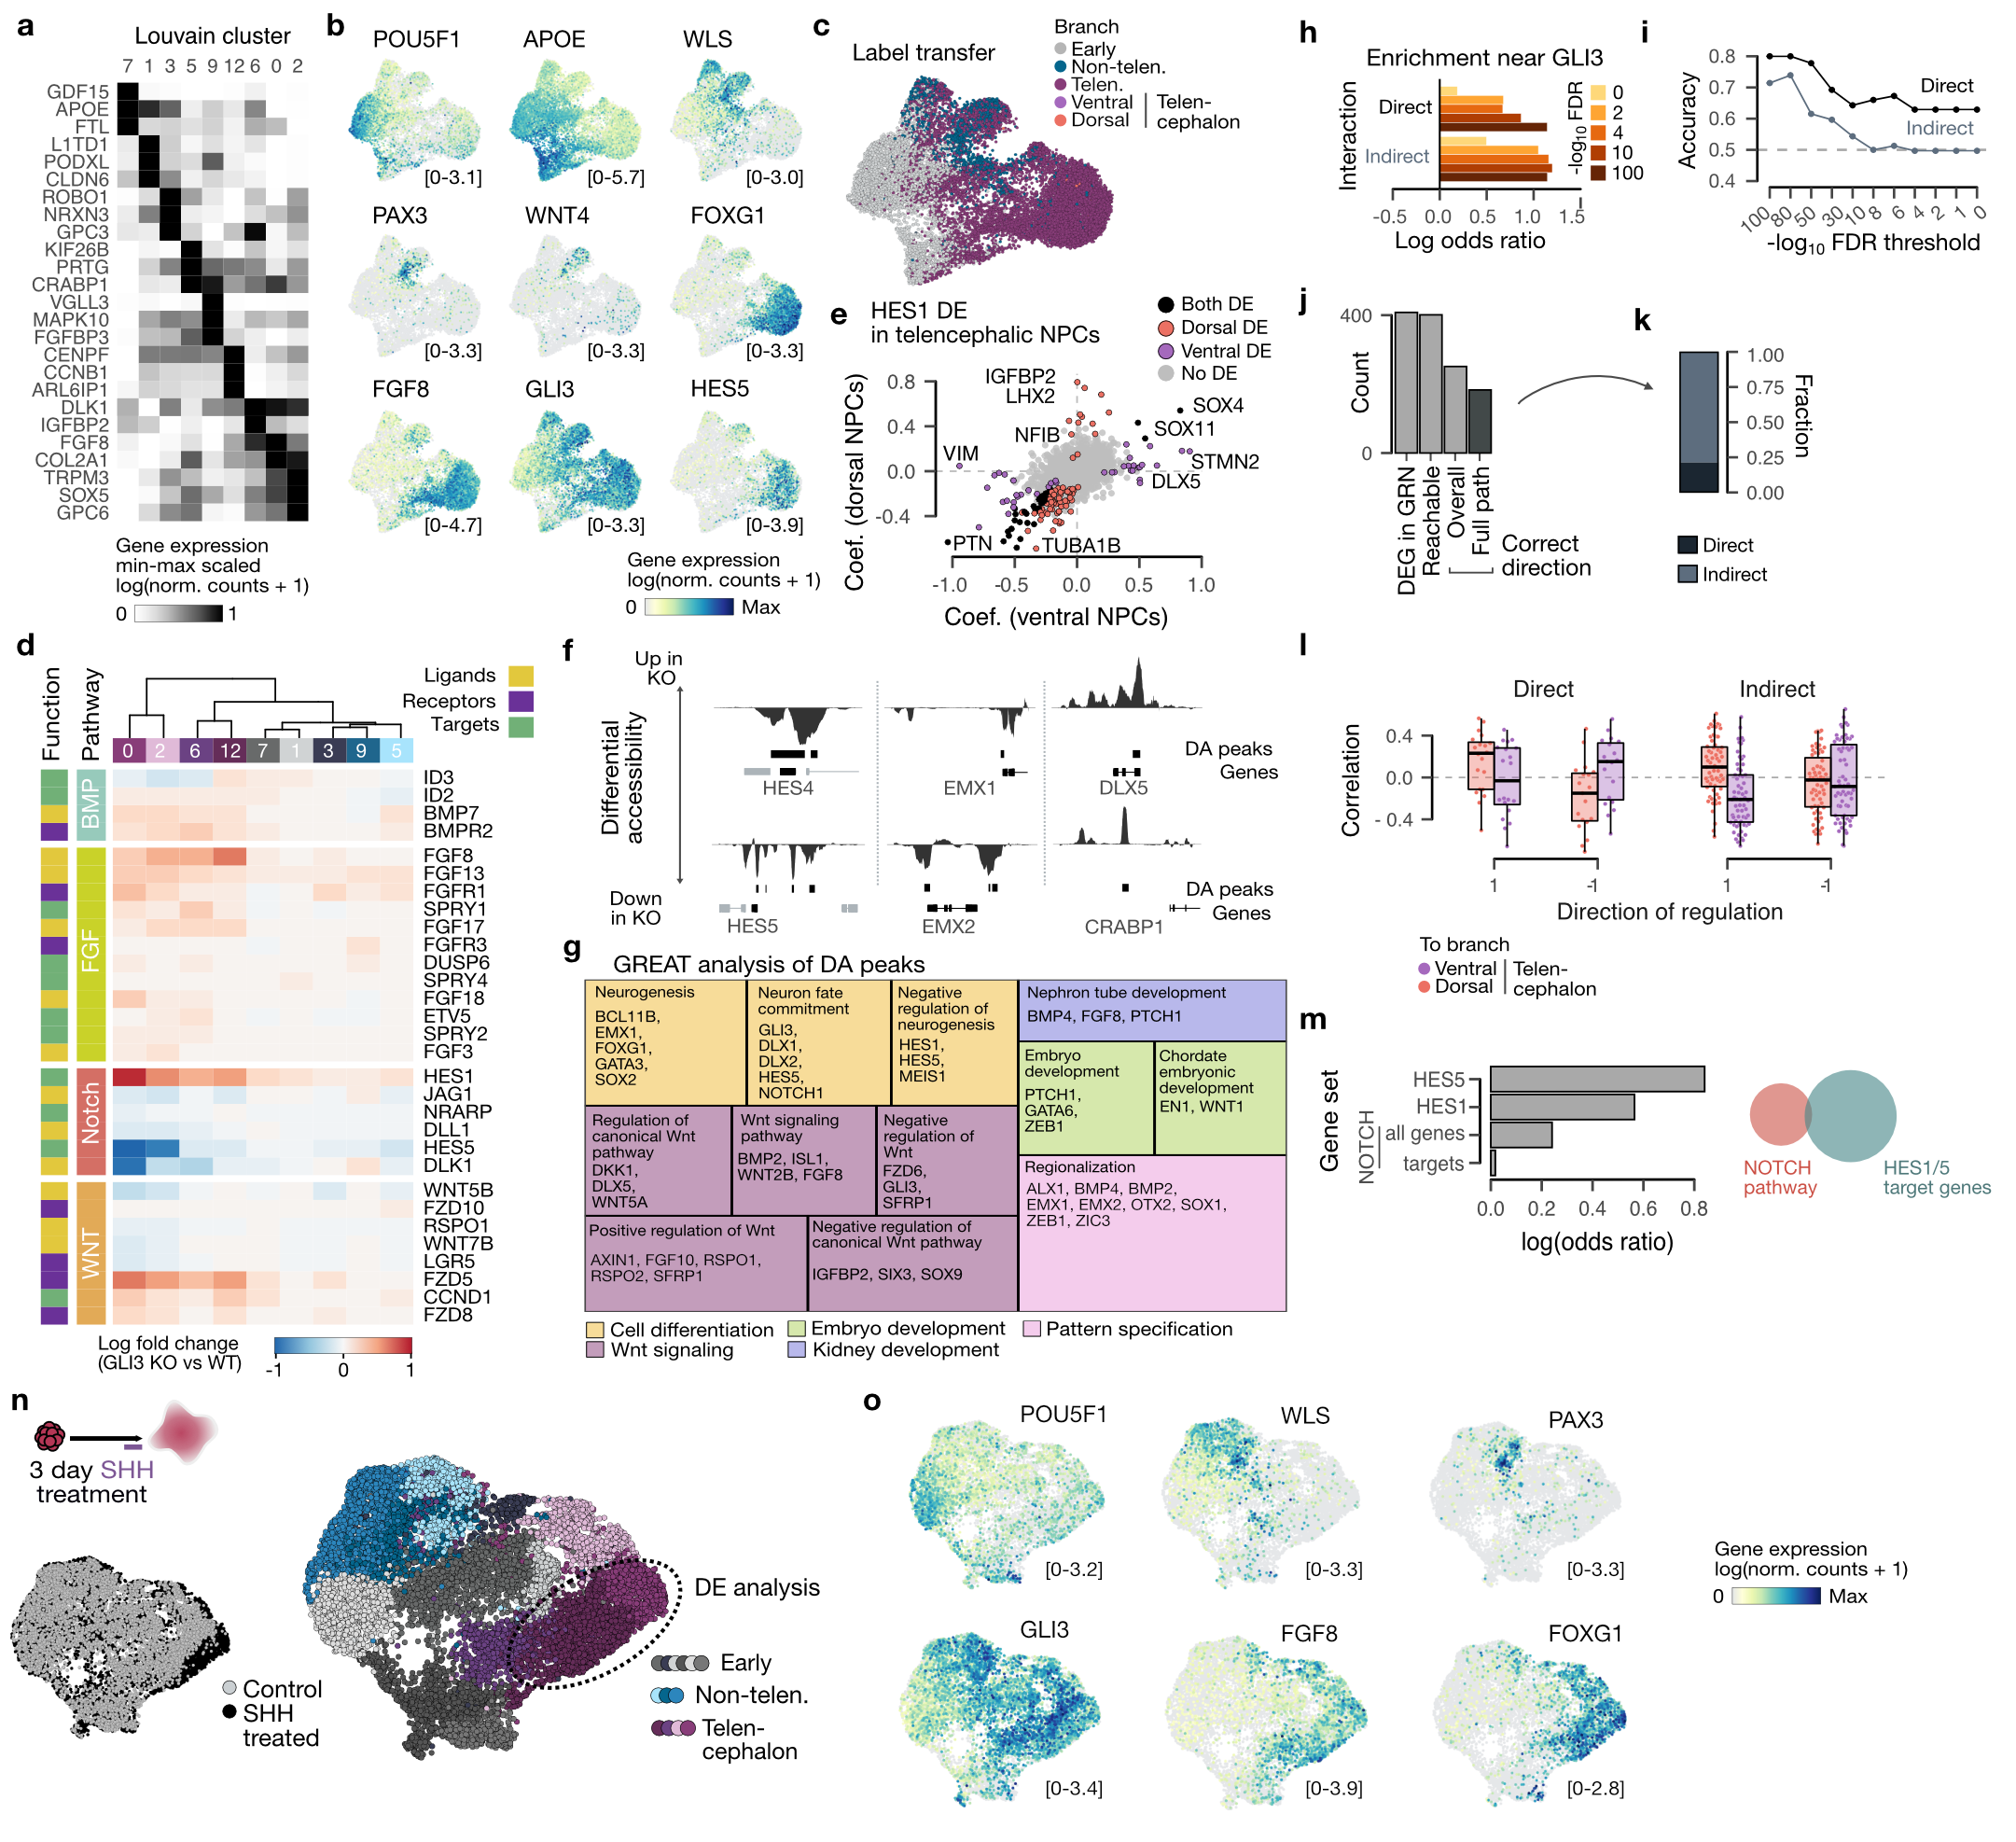
\includegraphics[width=\textwidth]{figures/pando/Figure_S10}
    \label{fig:regS10}
    \caption{\textbf{GLI3 KO induced changes in telencephalic progenitors in cerebral organoids.} a, Heatmap showing min-max scaled expression (log(transcript counts per 10k +1)) of marker genes for unbiased Louvain clusters. b,  UMAP colored by the expression of selected marker genes. The range of values is indicated for each plot. c, UMAP embedding colored by branch labels predicted by label transfer from the organoid time course. d, Heatmap showing DE associated with signaling pathways. e, Scatter plot showing DE in neural progenitor cells (NPCs) upon HES1 perturbation in the mosaic perturbation experiment. f, Signal tracks showing differentially accessible (DA) peaks in cluster 0 and 2. g, GREAT enrichment analysis of DA peaks in cluster 0 and 2, with box area proportional to FDR. Representative genes are shown. h, Enrichment of DE genes in the neighborhood of GLI3 in the GRN. i, Accuracy of GRN predicted directionality of GLI3 effect at different false discovery rate (FDR) thresholds. j, Barplot showing the number of all DE genes in the GRN (DEG in GRN), all DE genes reachable from GLI3 in the graph (Reachable), DE genes where the GRN was consistent with the DE result (Overall) and DE genes for which all subpaths from GLI3 were consistent with the DE result (Full path). k, Barplot showing the fraction of DE genes directly and indirectly regulated by GLI3. l, Boxplot showing the spearman correlation of directly (n=39) and indirectly (n=126) regulated DE genes with transition probabilities ventral and dorsal branched. The center line represents the median, boxes indicate 25\%-75\% interquantile range and whiskers 1.5 * interquantile range. m, Barplot showing the enrichment of gene sets (HES1/5 target genes, NOTCH components) among telencephalic DE genes. n, UMAP embedding showing annotation of multiome SHH experiment. o, UMAP colored by the expression of selected marker genes.}
\end{figure}

\clearpage

\topparagraph{Supplementary Data}

\noindent
All supplementary data items can be obtained from polybox with the following link: \\ \href{https://polybox.ethz.ch/index.php/s/5ZbTkjaiCl1XUvr}{https://polybox.ethz.ch/index.php/s/5ZbTkjaiCl1XUvr} 

\vspace{0.5cm}
\noindent
{\normalfont\footnotesize\sffamily\textbf{Supplementary Data Figure 3.3.1 | Raw data western blots.} Red boxes indicate cropped areas shown in Figure S3.9.} 

\vspace{0.25cm}
\noindent
{\normalfont\footnotesize\sffamily\textbf{Supplementary Table 3.1 | Overview of single-cell genomic experiments.}}

\vspace{0.25cm}
\noindent
{\normalfont\footnotesize\sffamily\textbf{Supplementary Table 3.2 | Feature sets used for integration and GRN inference.}}

\vspace{0.25cm}
\noindent
{\normalfont\footnotesize\sffamily\textbf{Supplementary Table 3.3 | Stage-specific features.}}

\vspace{0.25cm}
\noindent
{\normalfont\footnotesize\sffamily\textbf{Supplementary Table 3.4 | GO enrichments for stage-specific genomic regions.}}

\vspace{0.25cm}
\noindent
{\normalfont\footnotesize\sffamily\textbf{Supplementary Table 3.5 | Enrichment effects in the CROP-seq screen. }P-values were derived using a Cochran-Mantel-Haenzel test and FDR-correction.}

\vspace{0.25cm}
\noindent
{\normalfont\footnotesize\sffamily\textbf{Supplementary Table 3.6 | Transcriptomic KO effects in the CROP-seq screen.} P-values were derived using ANOVA and FDR-correction.}

\vspace{0.25cm}
\noindent
{\normalfont\footnotesize\sffamily\textbf{Supplementary Table 3.7 | Functional enrichments for E2F2 KO effects.} P-values were derived from DAVID, which uses a a modified one-sided Fisher's exact test.}

\vspace{0.25cm}
\noindent
{\normalfont\footnotesize\sffamily\textbf{Supplementary Table 3.8 | Differential expression in ventral telencephalon neurons upon GLI3 KO.} P-values were derived using ANOVA and FDR-correction.}

\vspace{0.25cm}
\noindent
{\normalfont\footnotesize\sffamily\textbf{Supplementary Table 3.9 | Differential expression in early telencephalic progenitors upon GLI3 KO.} P-values were derived using ANOVA and FDR-correction.}

\vspace{0.25cm}
\noindent
{\normalfont\footnotesize\sffamily\textbf{Supplementary Table 3.10 | Differential accessibility in early telencephalic progenitors upon GLI3 KO.} P-values were derived using a likelihood-ratio test and FDR-correction.}

\vspace{0.25cm}
\noindent
{\normalfont\footnotesize\sffamily\textbf{Supplementary Table 3.11 | GO enrichments for differentially accessible genomic regions in GLI3 KO.} P-values were derived using a hypergeometric test and FDR-correction as well as Bonferroni-correction.}



 









